% Copyright (c) 2014,2016 Casper Ti. Vector
% Public domain.

\section{Check of the background PDF on $B$ mass sidebands}
\label{SUPPsec:app_B_sideband}

As described before, the 6D background PDF is constructed using
the $B$ mass sideband events, assuming that it can be factorized into a product of
2D functions of $m_{\phi K}$ and decay angles in the $K^*$ decay chain.
Such constructed 6D background density is then divided by similarly constructed
6D selection efficiency parametrization, worked out using the simulated events,
and then added to the signal matrix element squared
in a proportion constrained by the background fraction in the real data sample.
To cross-check how well such background PDF describes the sideband distributions
we show in Fig.~\ref{fig:mass_distribution_phi_sideband}
its projections onto the masses and decay angles from
all three chains superimposed on the sideband data.
The projections are achieved by weighting the phase-space MC events, passed
through the selection criteria, by the parameterized background PDF.
Since the $X$ and $Z$ decay chain variables are not used in the parameterization of the background PDF,
the cross-check is non-trivial.
The cross-check also depends on the cancellation of the parameterized efficiency in the background PDF
by the unparameterized efficiency encoded in the MC events, which is a part of our cFit approach.
The agreement is fairly reasonable.

\begin{figure}[!hbtp]
\centering
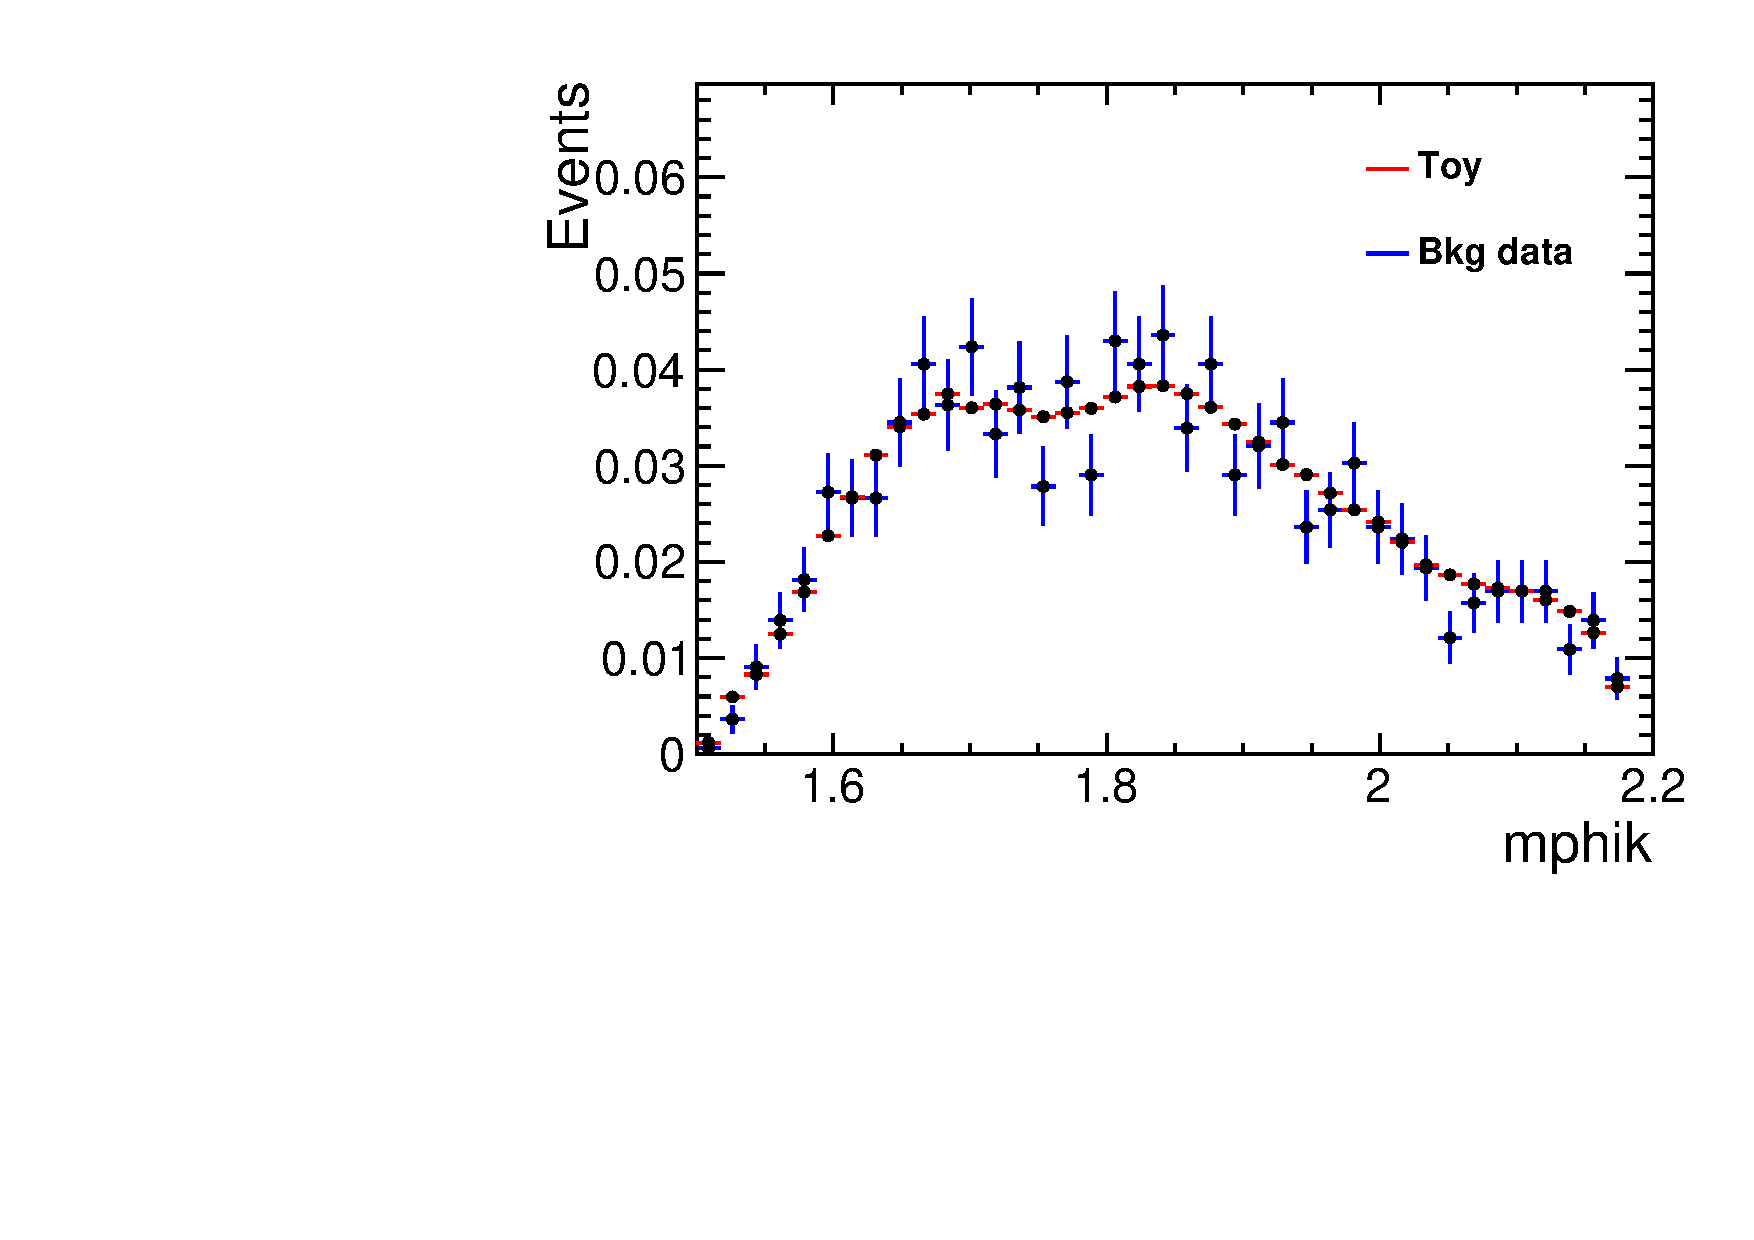
\includegraphics[width=0.3\textwidth]{Figures/03_Zcs/app_sideband/mphik.pdf}  %
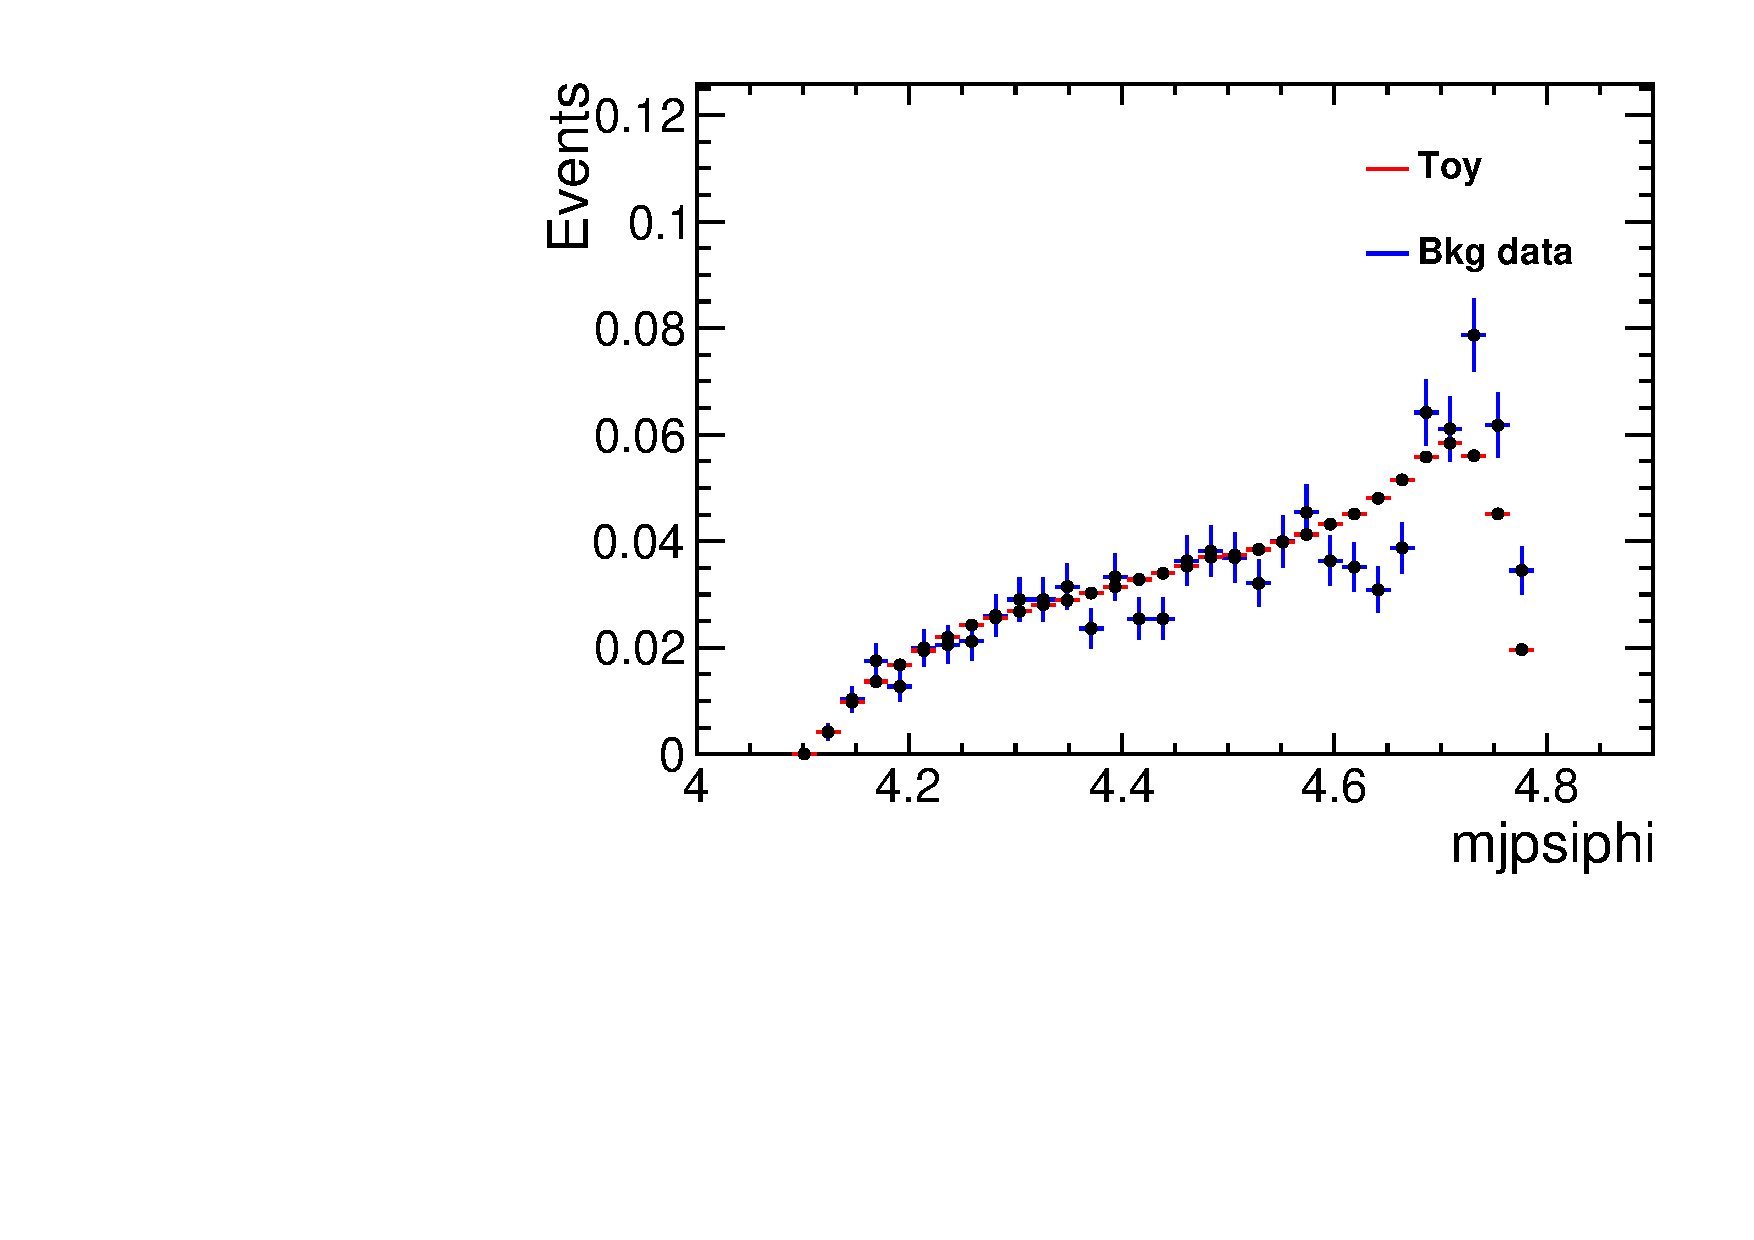
\includegraphics[width=0.3\textwidth]{Figures/03_Zcs/app_sideband/mjpsiphi.pdf}  %
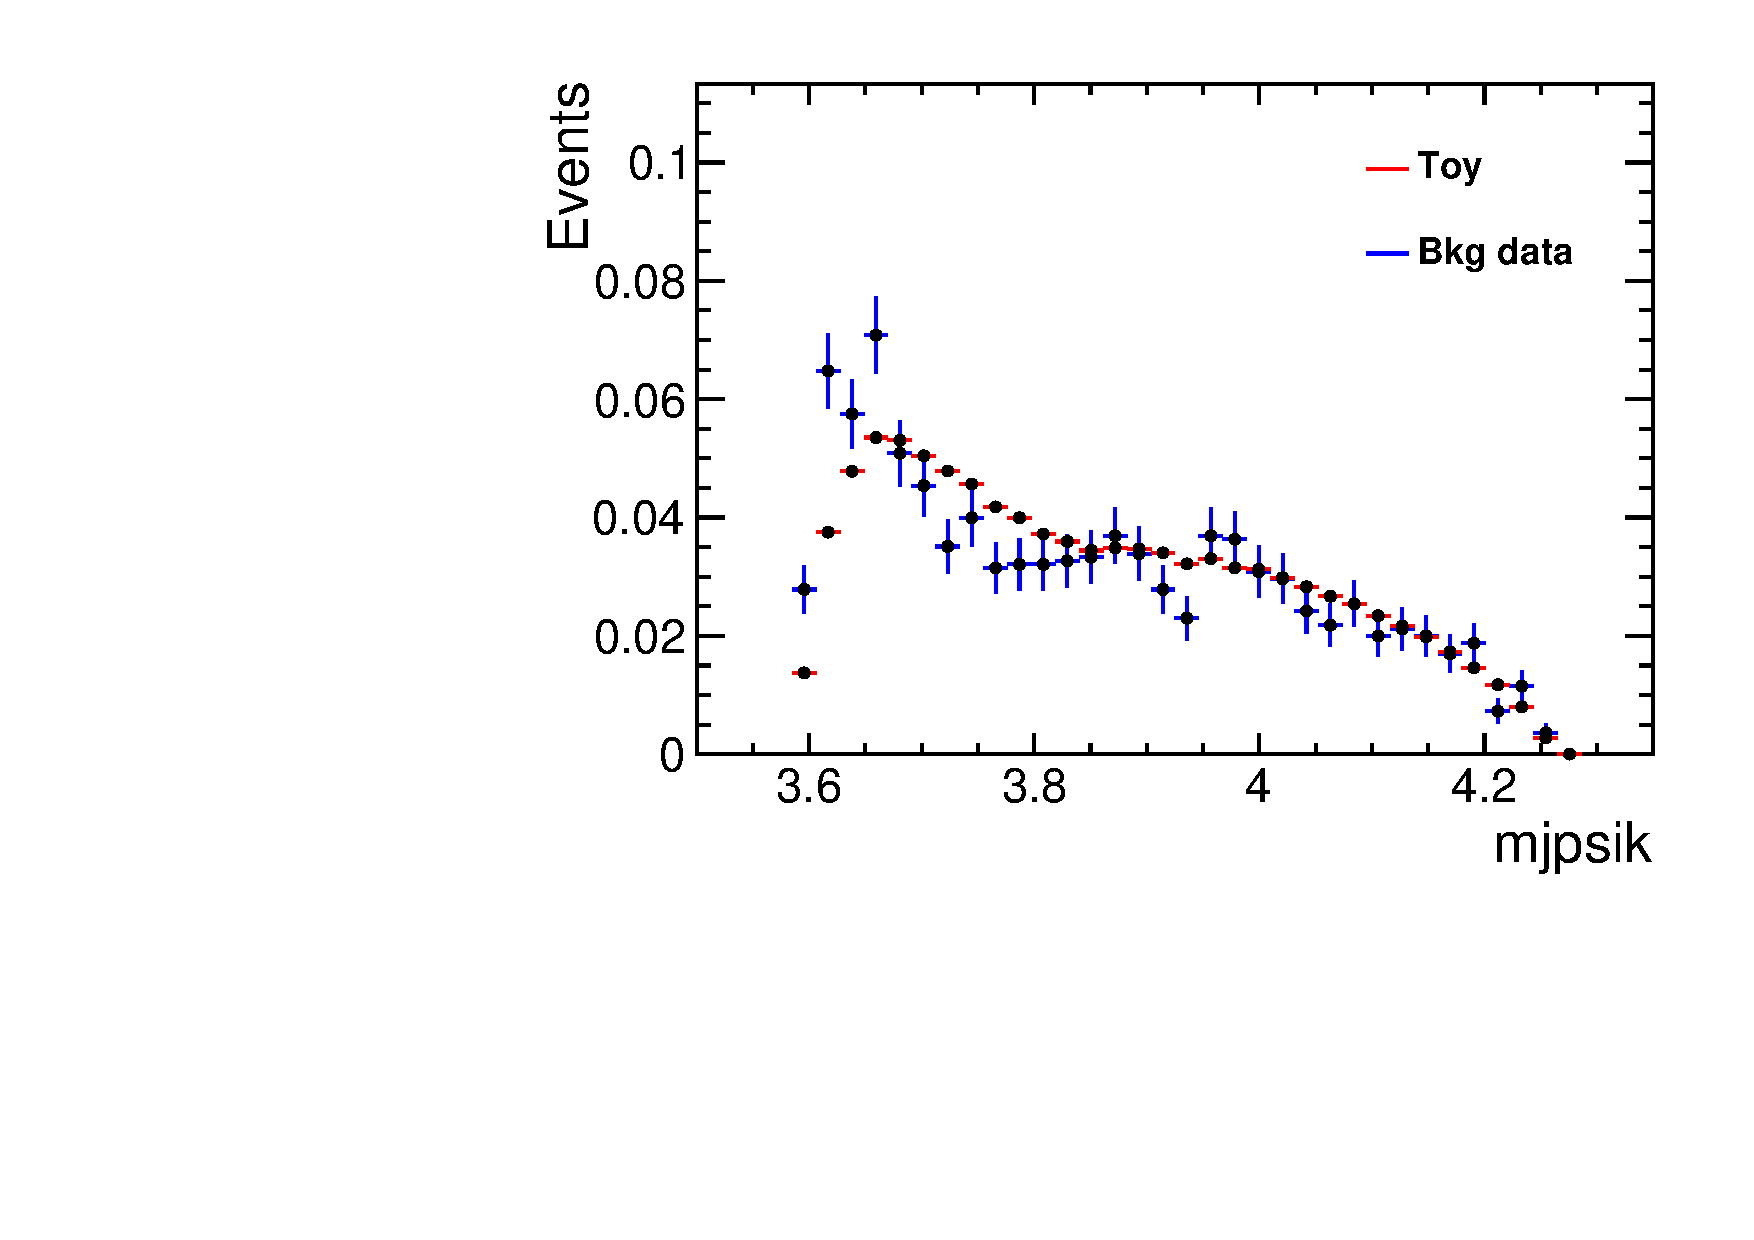
\includegraphics[width=0.3\textwidth]{Figures/03_Zcs/app_sideband/mjpsik.pdf} \\
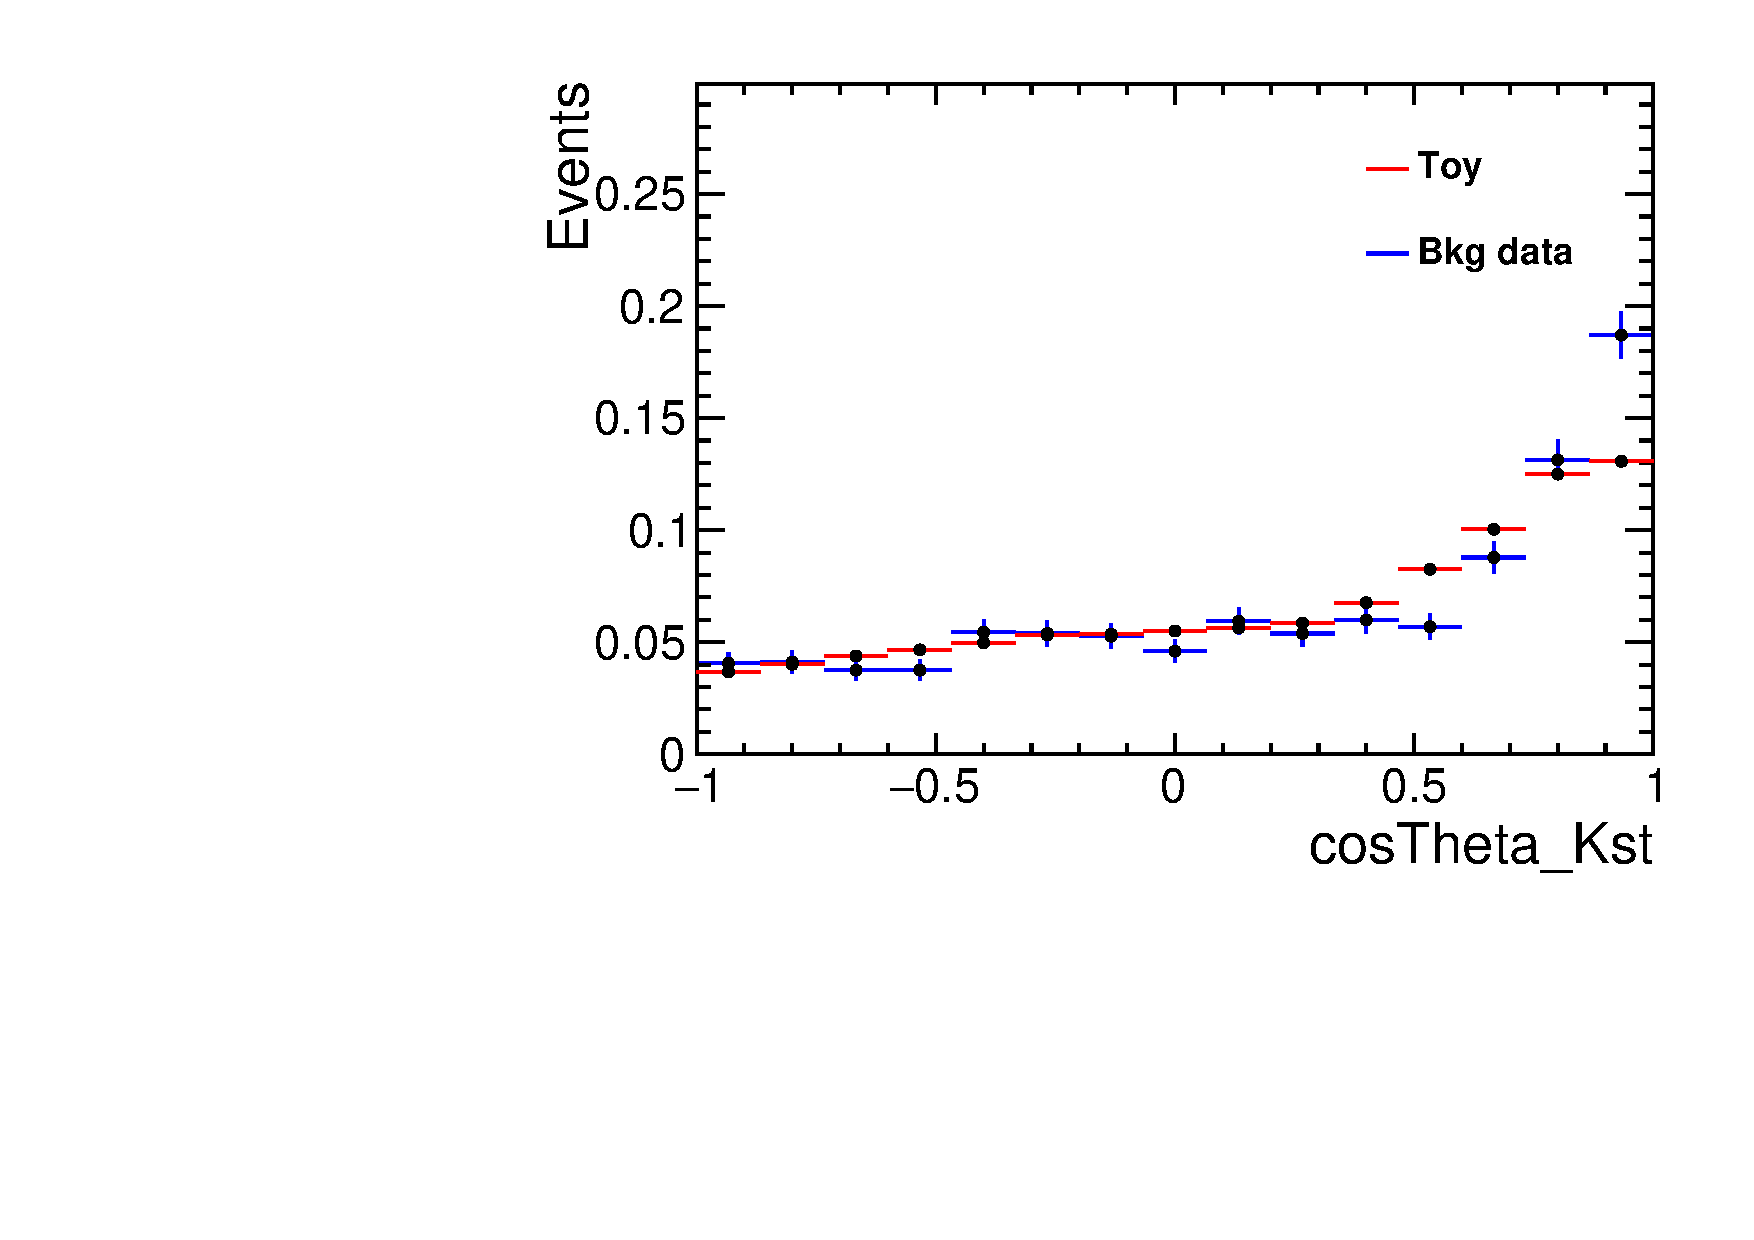
\includegraphics[width=0.3\textwidth]{Figures/03_Zcs/app_sideband/cosTheta_Kst.pdf}%
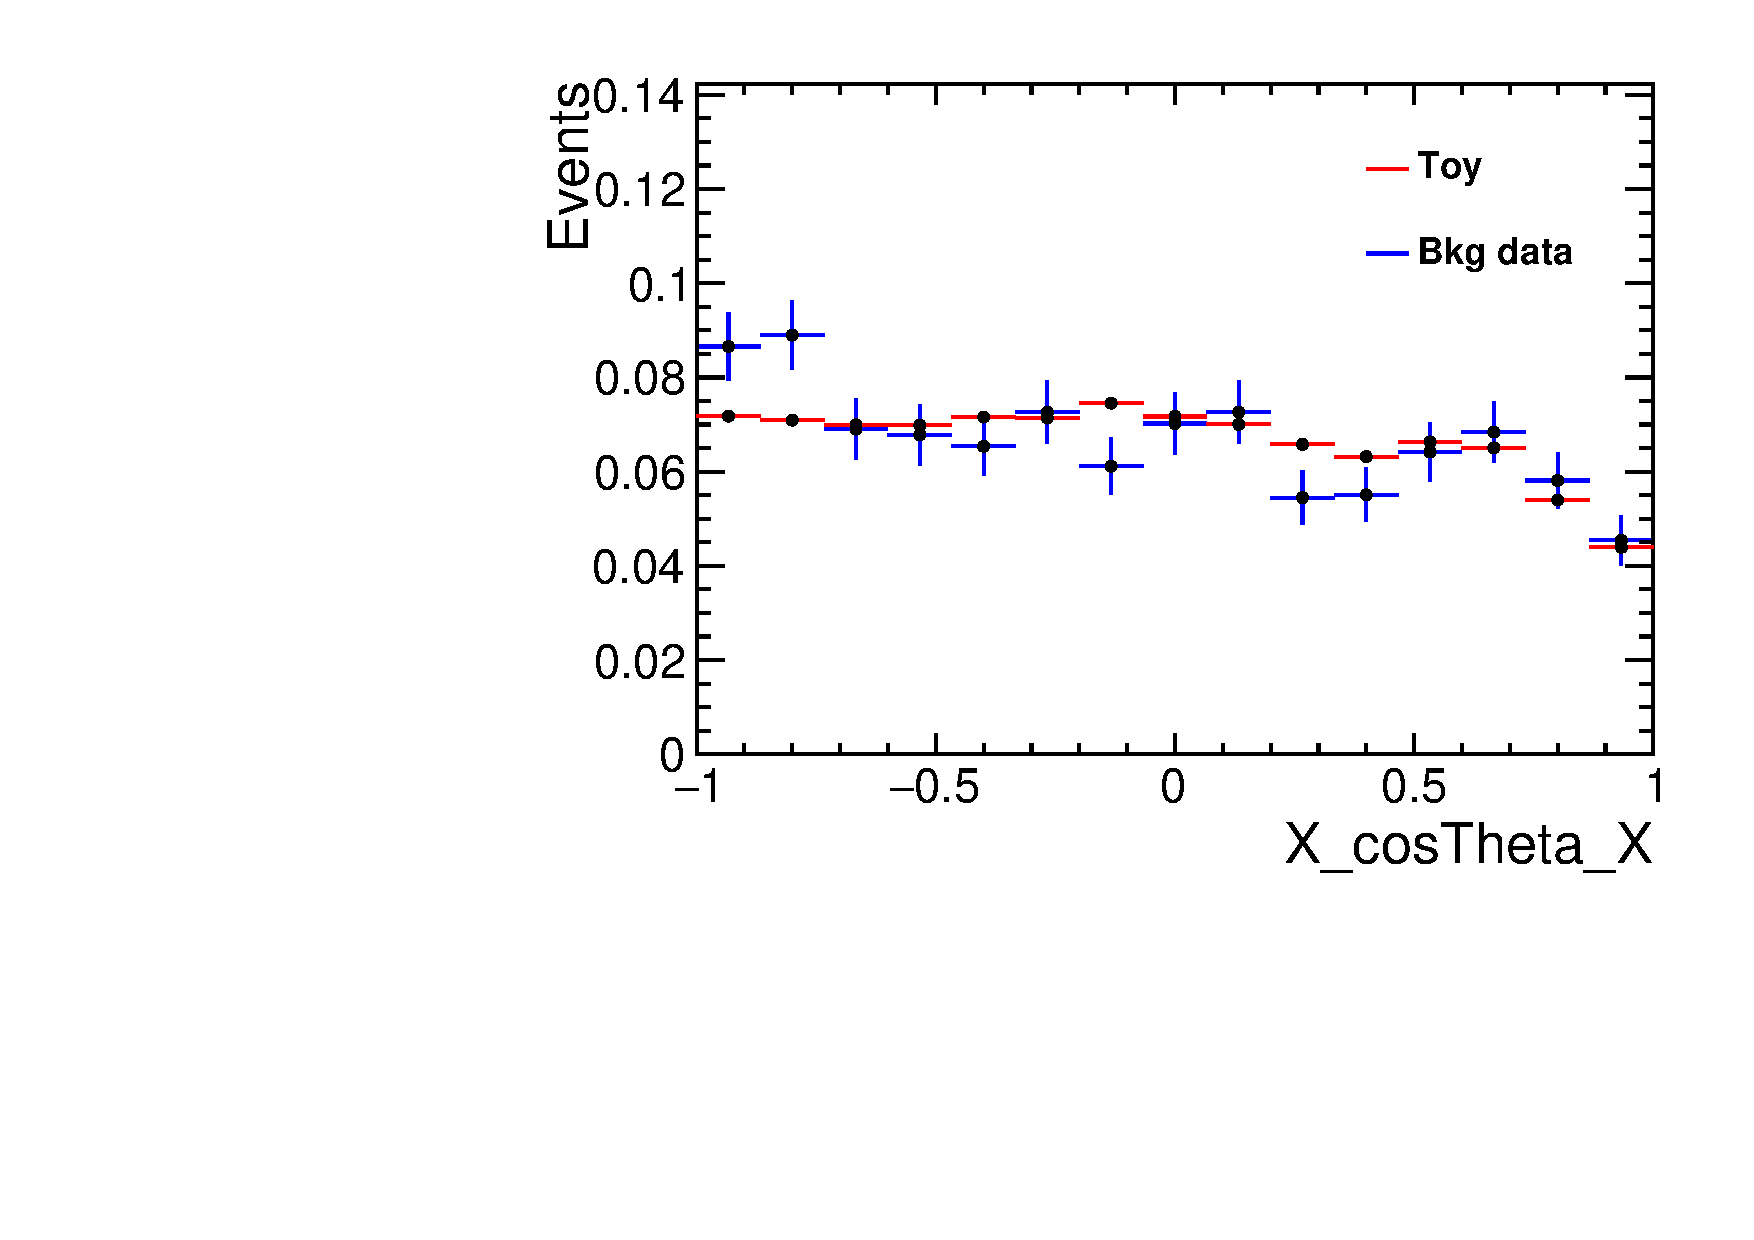
\includegraphics[width=0.3\textwidth]{Figures/03_Zcs/app_sideband/X_cosTheta_X.pdf}%
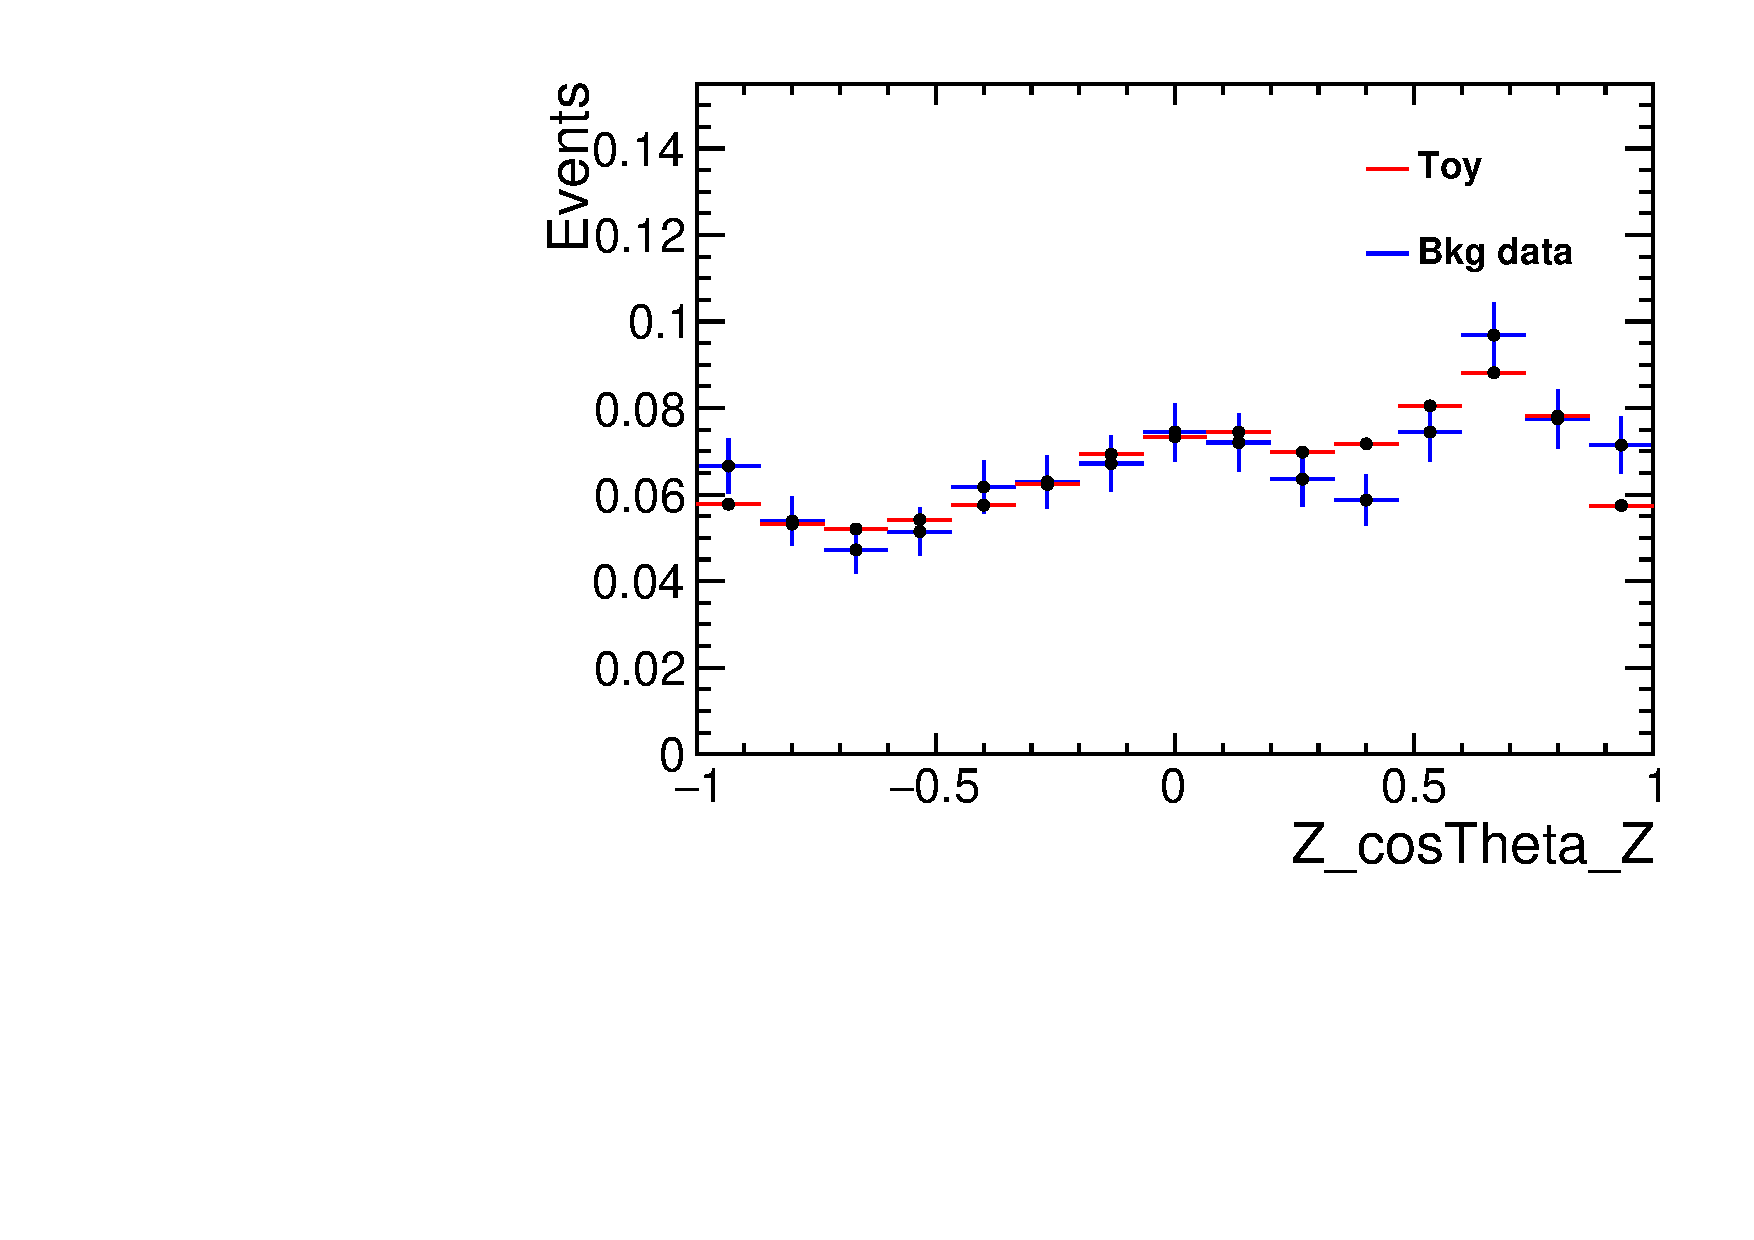
\includegraphics[width=0.3\textwidth]{Figures/03_Zcs/app_sideband/Z_cosTheta_Z.pdf} \\%
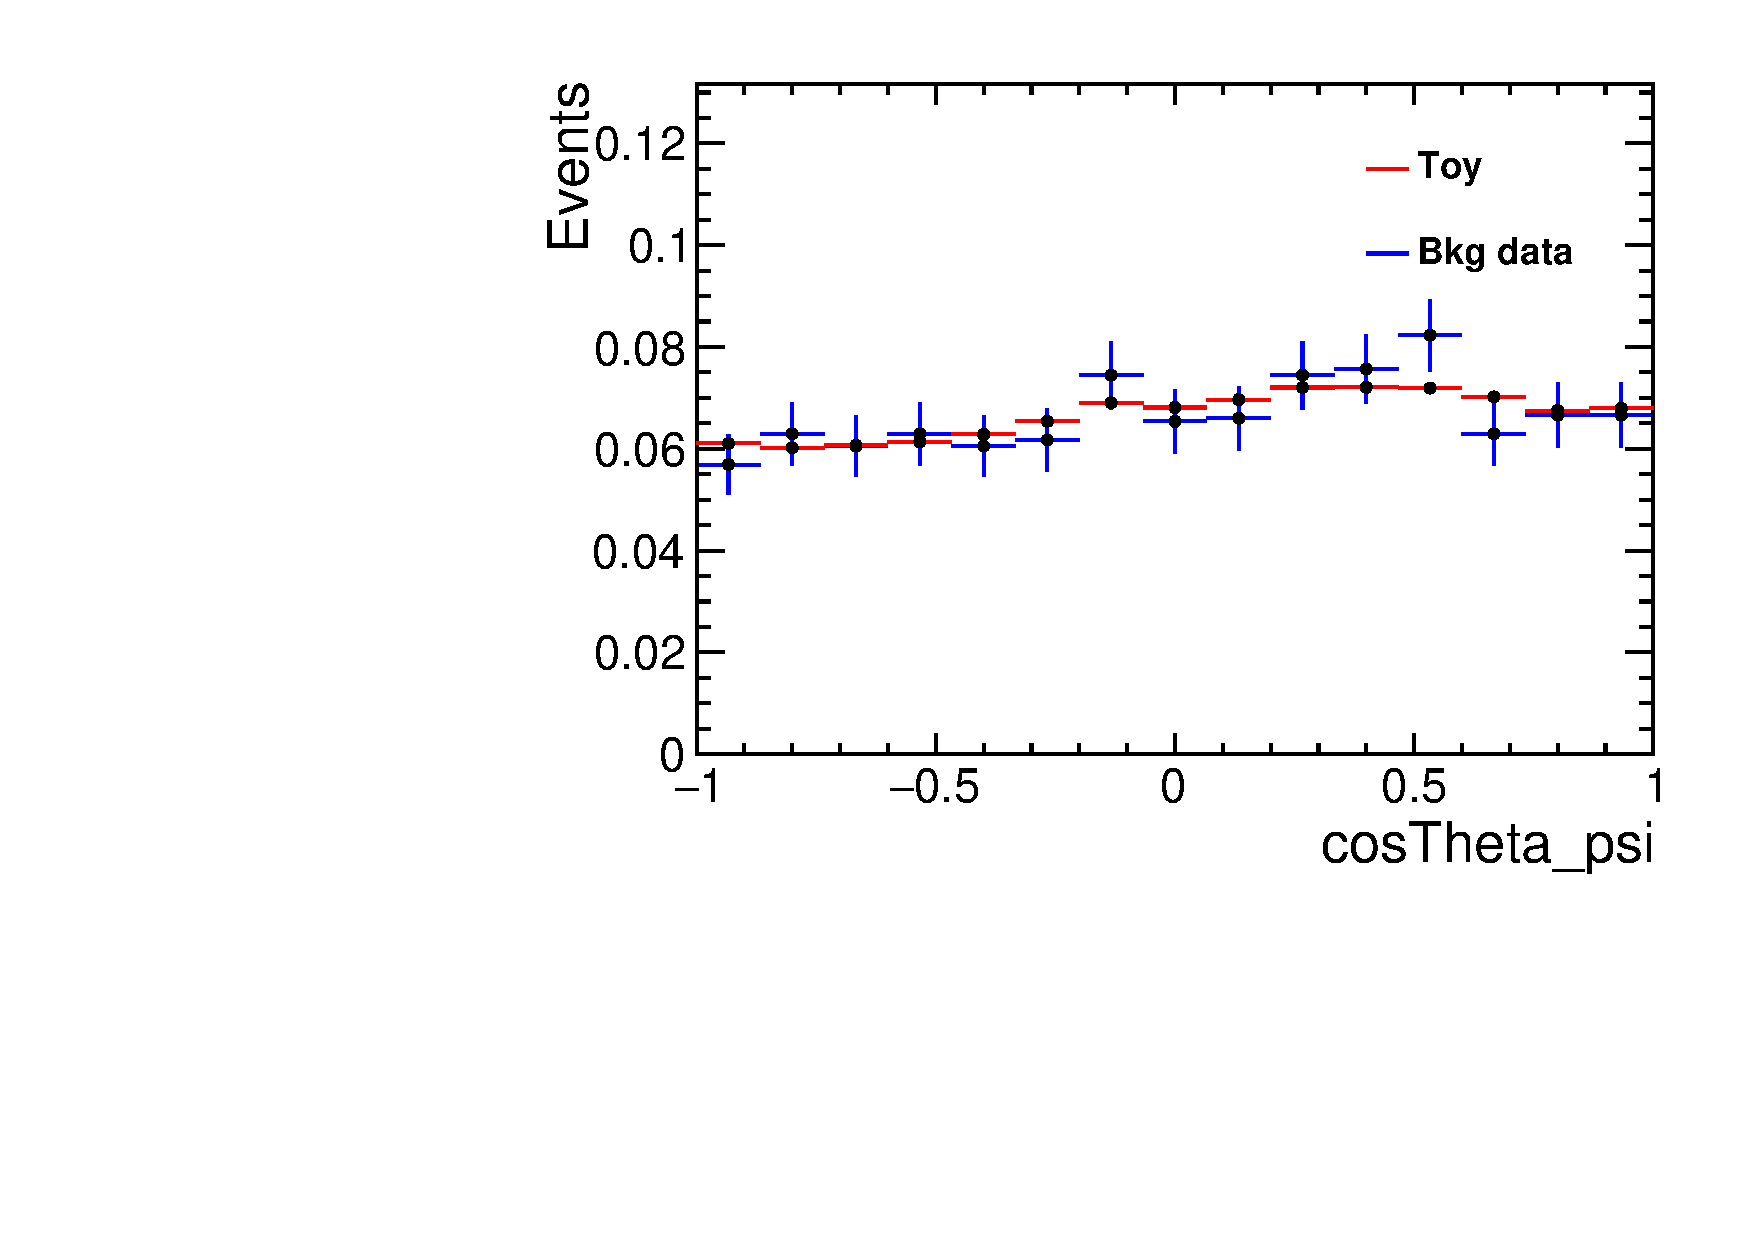
\includegraphics[width=0.3\textwidth]{Figures/03_Zcs/app_sideband/cosTheta_psi.pdf}%
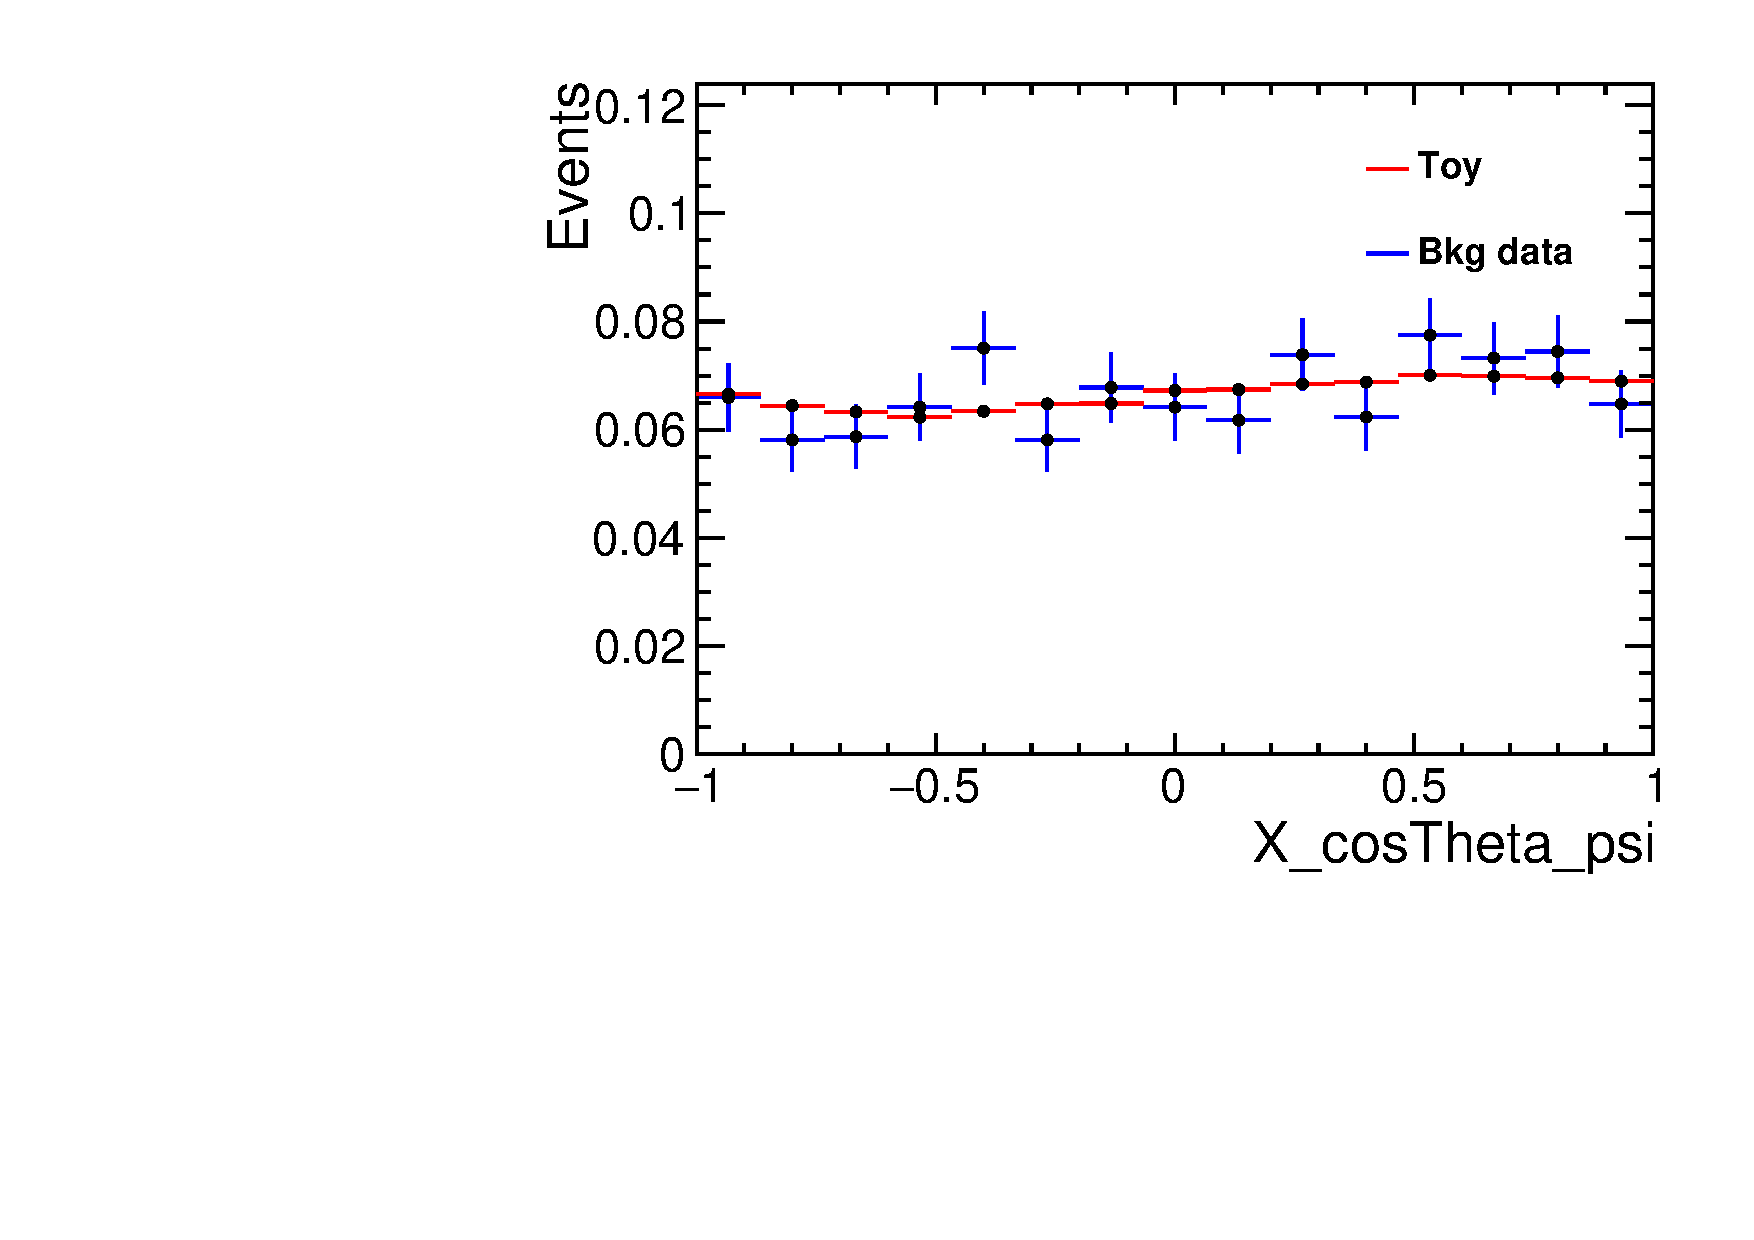
\includegraphics[width=0.3\textwidth]{Figures/03_Zcs/app_sideband/X_cosTheta_psi.pdf}%
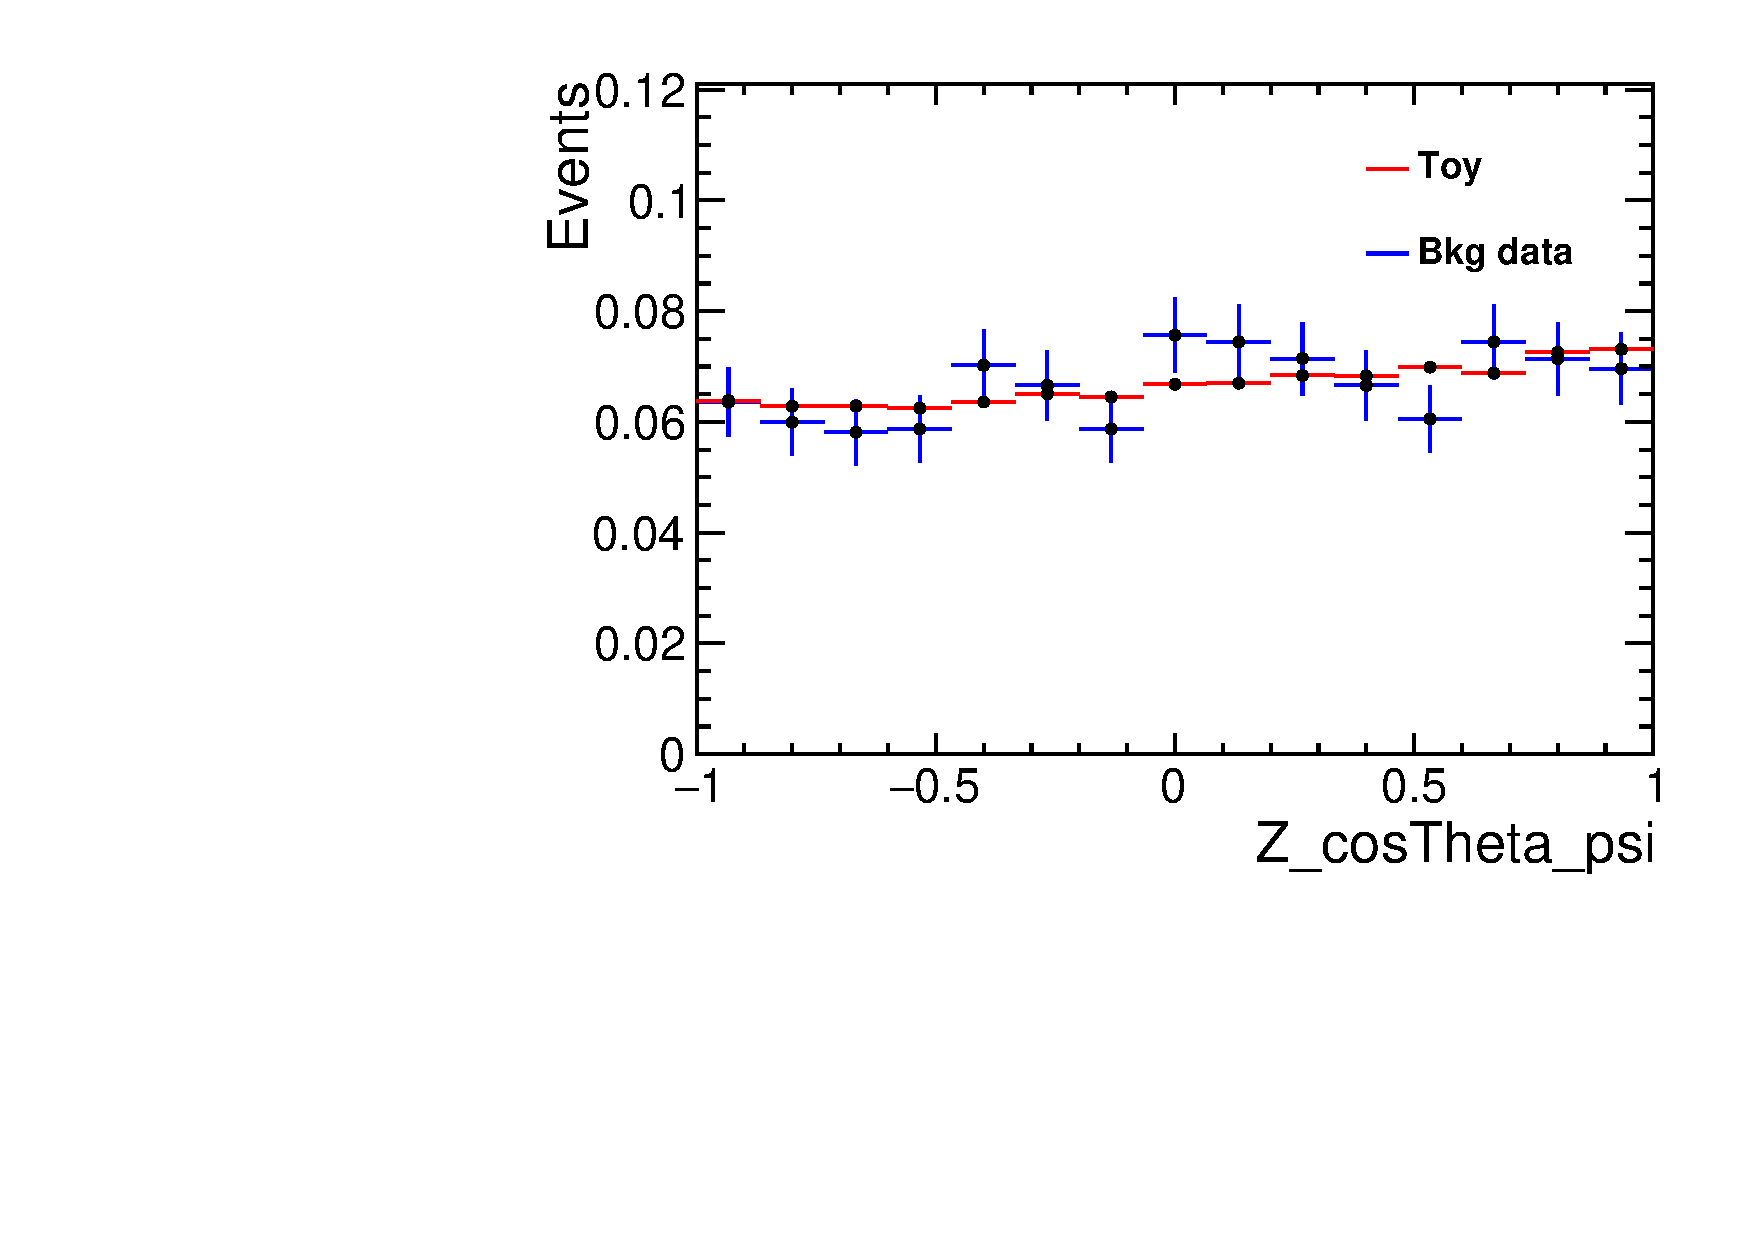
\includegraphics[width=0.3\textwidth]{Figures/03_Zcs/app_sideband/Z_cosTheta_psi.pdf}\\
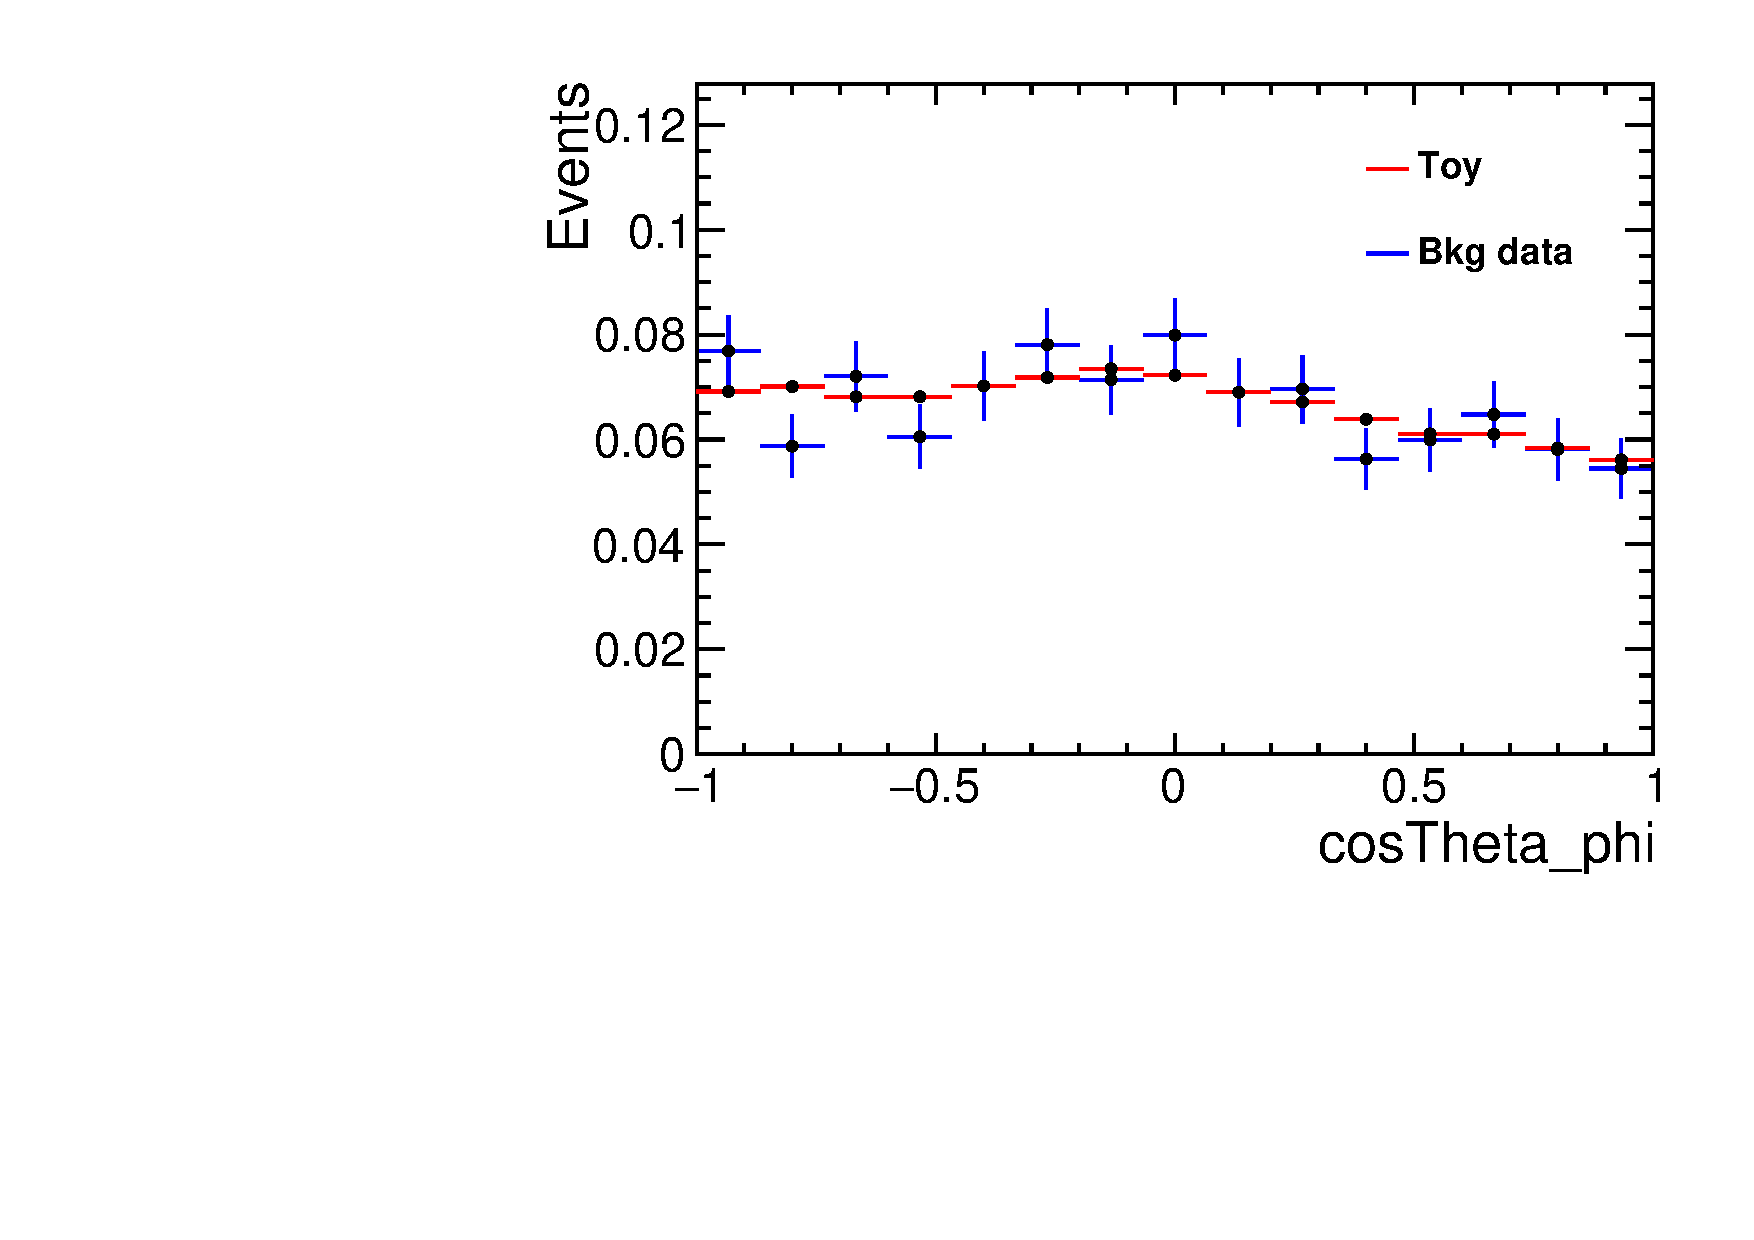
\includegraphics[width=0.3\textwidth]{Figures/03_Zcs/app_sideband/cosTheta_phi.pdf}%
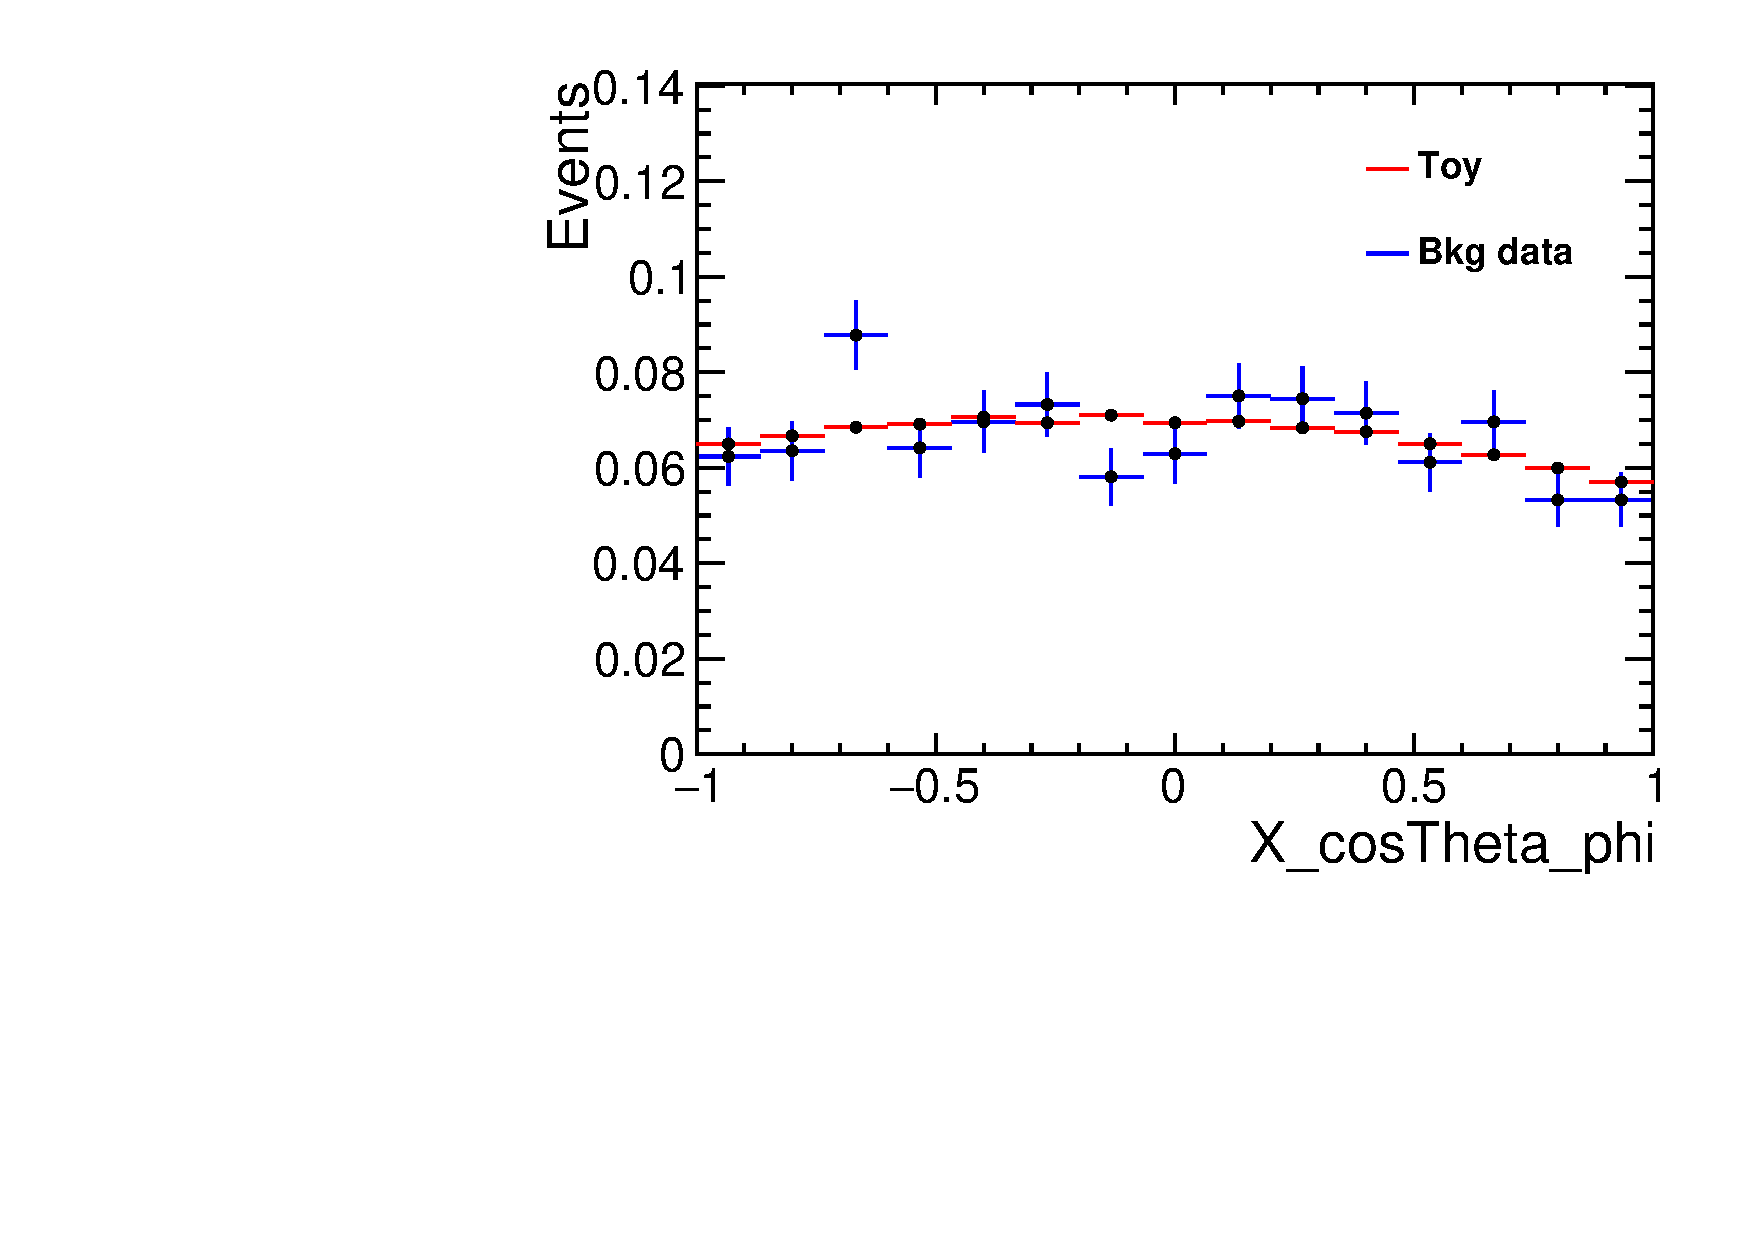
\includegraphics[width=0.3\textwidth]{Figures/03_Zcs/app_sideband/X_cosTheta_phi.pdf}%
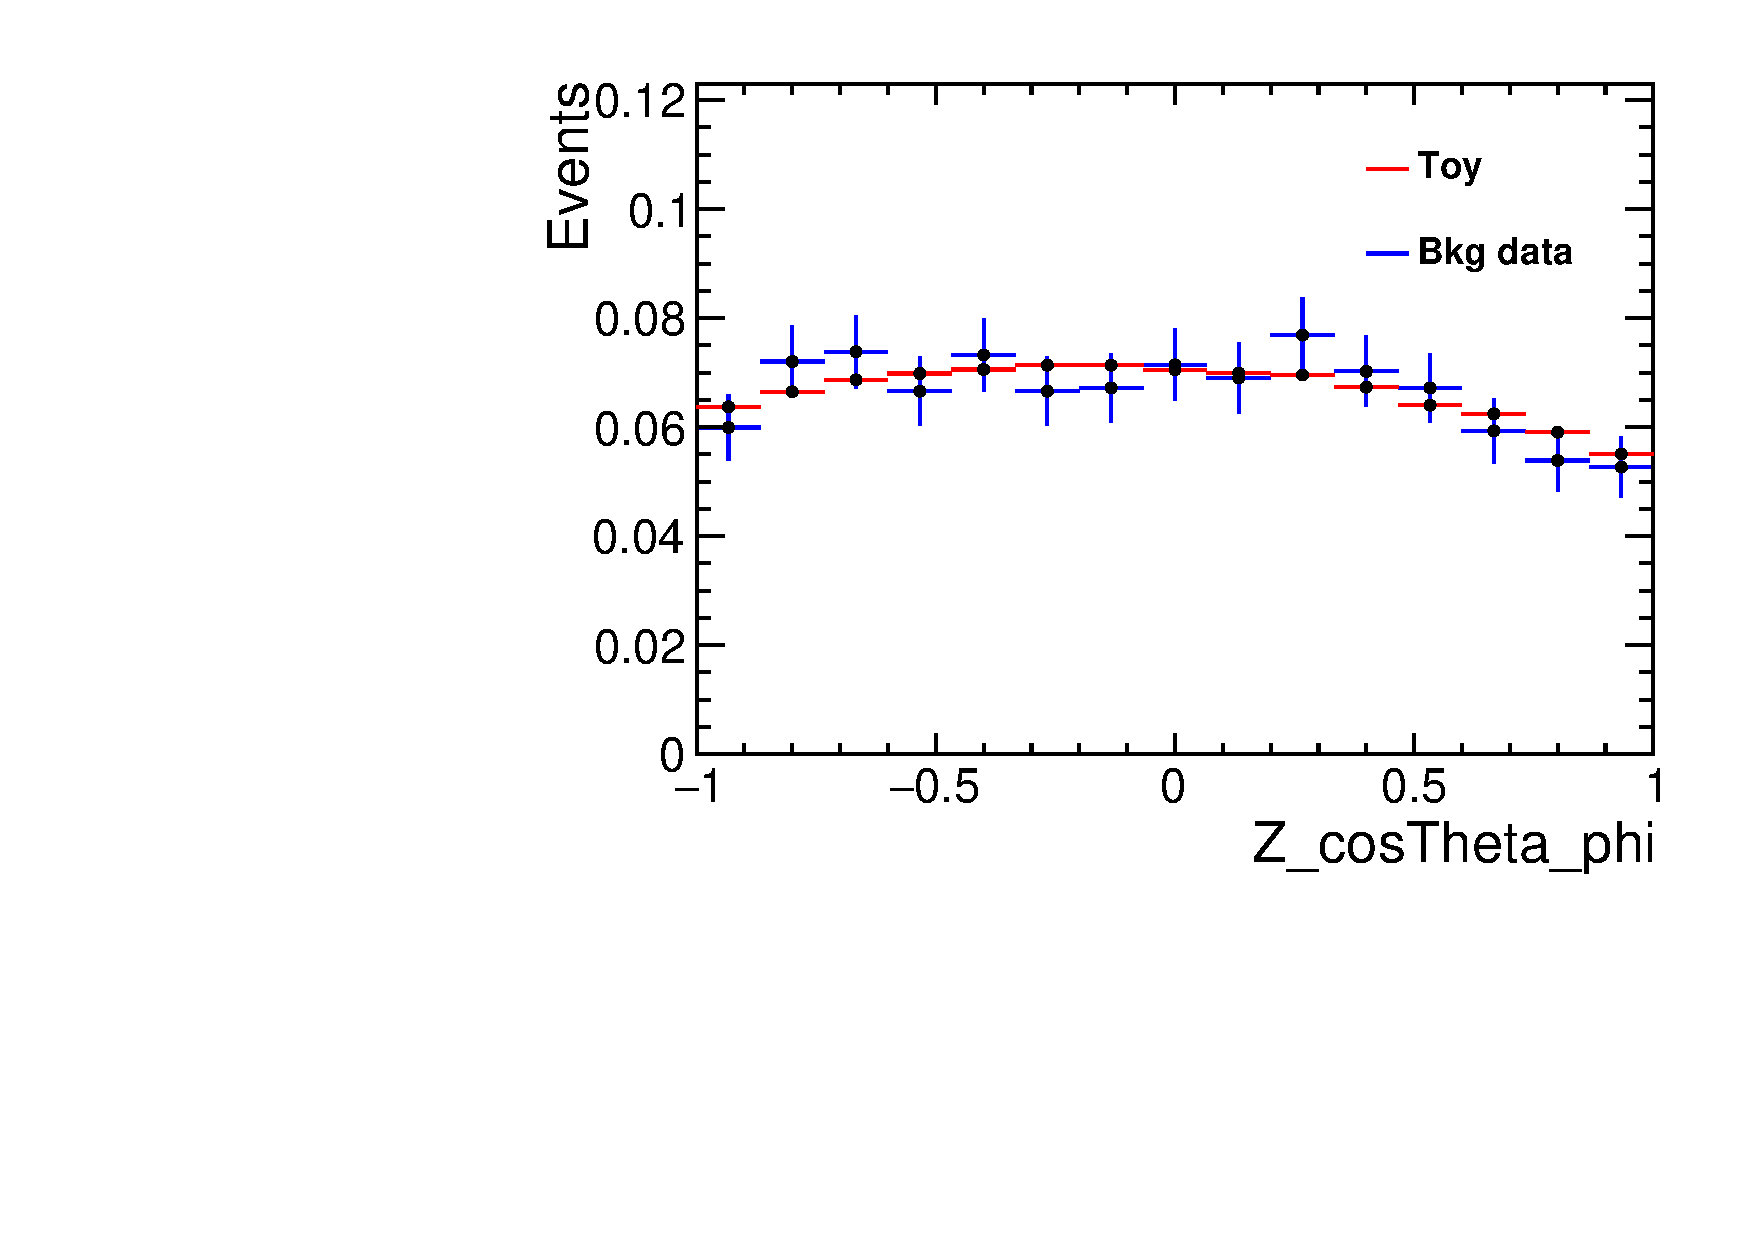
\includegraphics[width=0.3\textwidth]{Figures/03_Zcs/app_sideband/Z_cosTheta_phi.pdf}\\
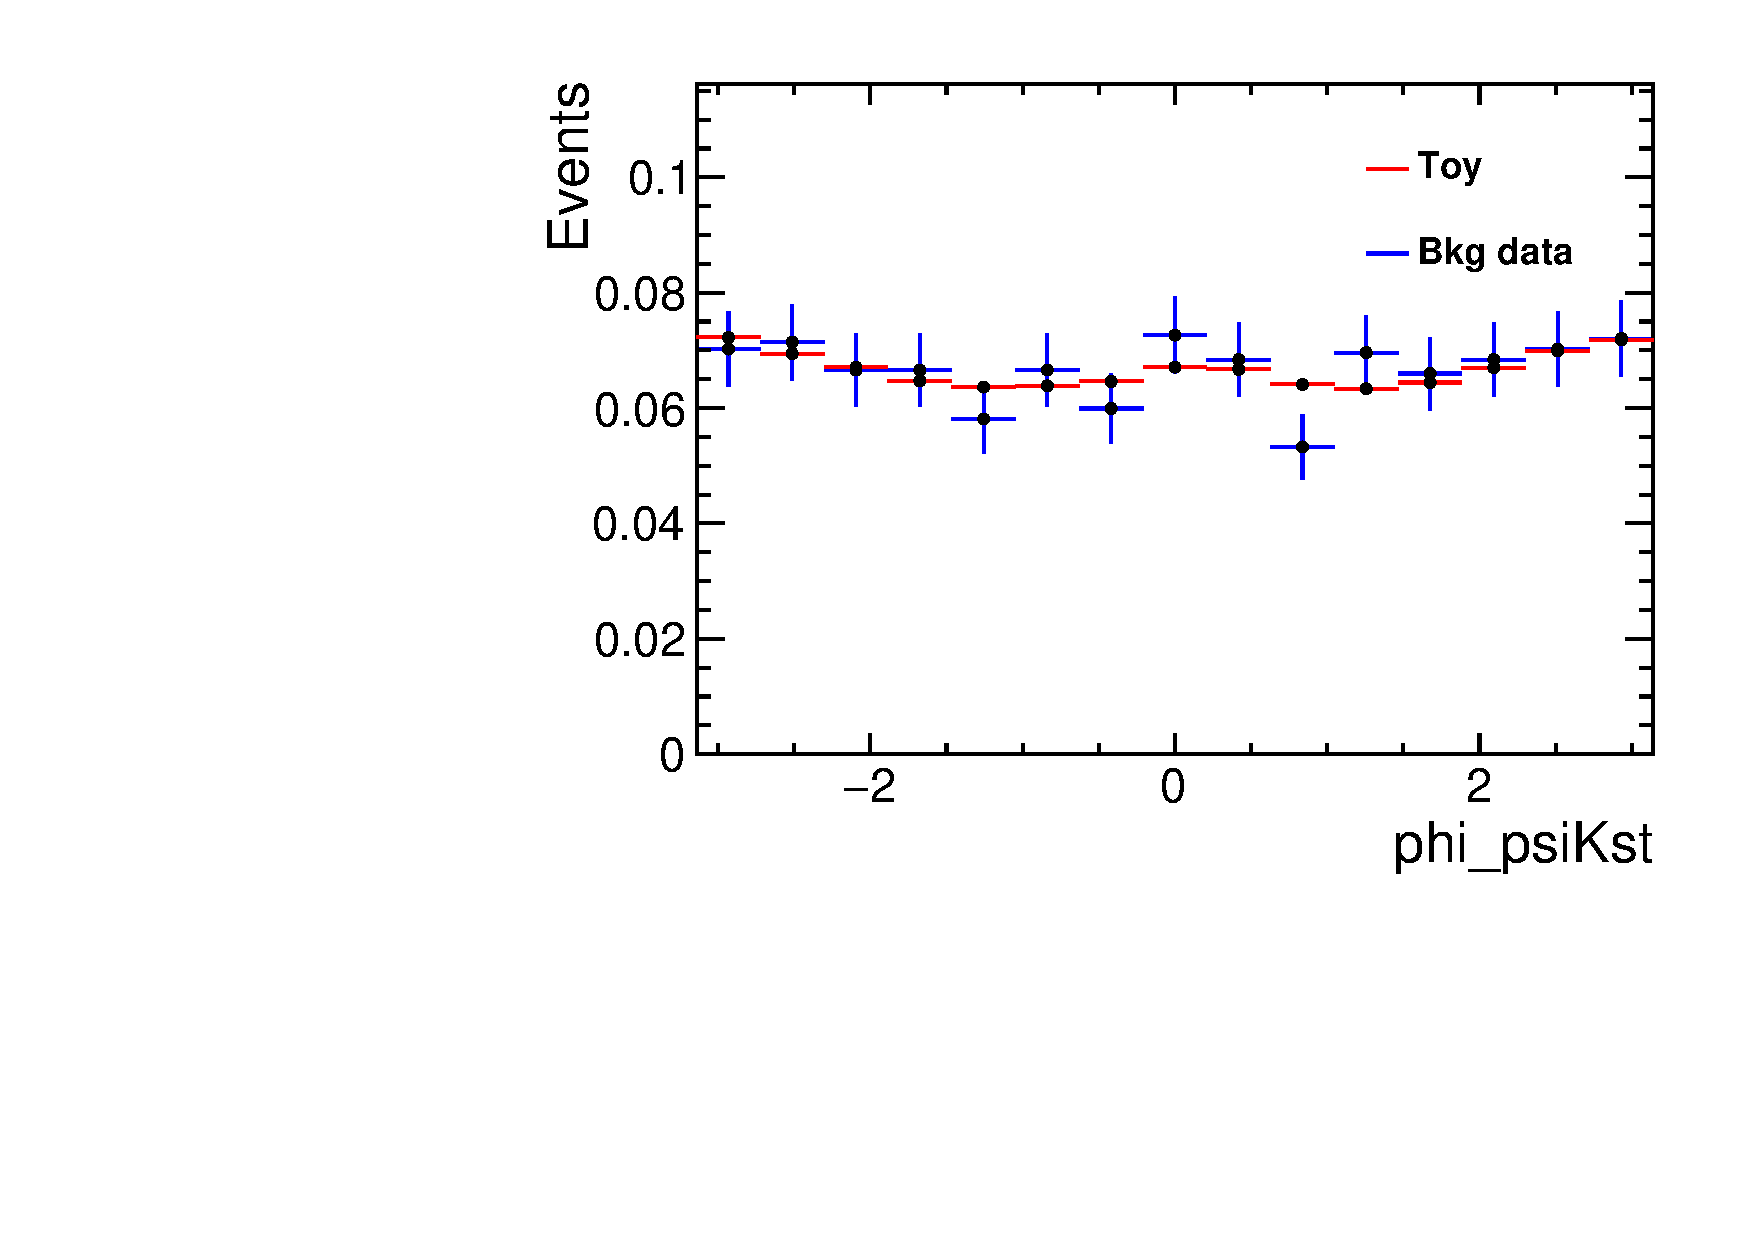
\includegraphics[width=0.3\textwidth]{Figures/03_Zcs/app_sideband/phi_psiKst.pdf}%
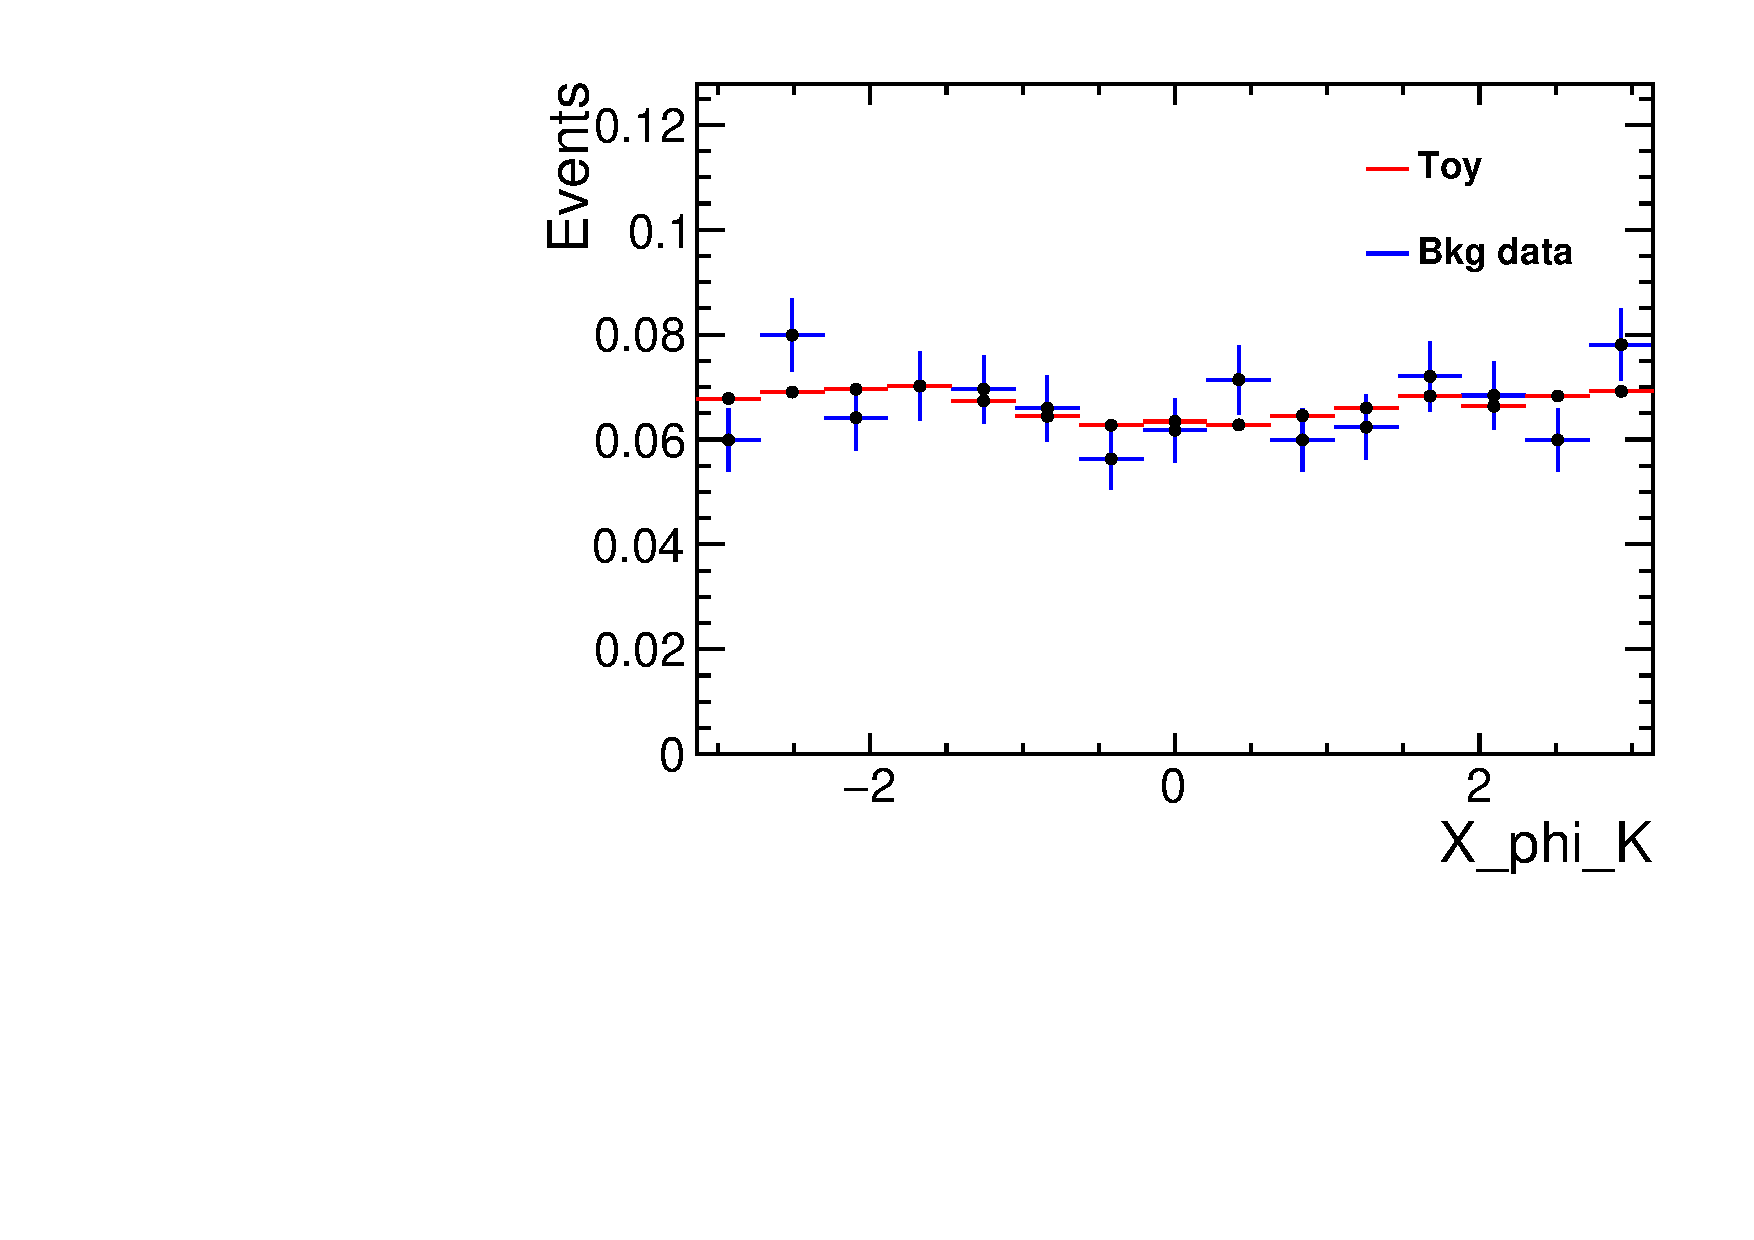
\includegraphics[width=0.3\textwidth]{Figures/03_Zcs/app_sideband/X_phi_K.pdf}%
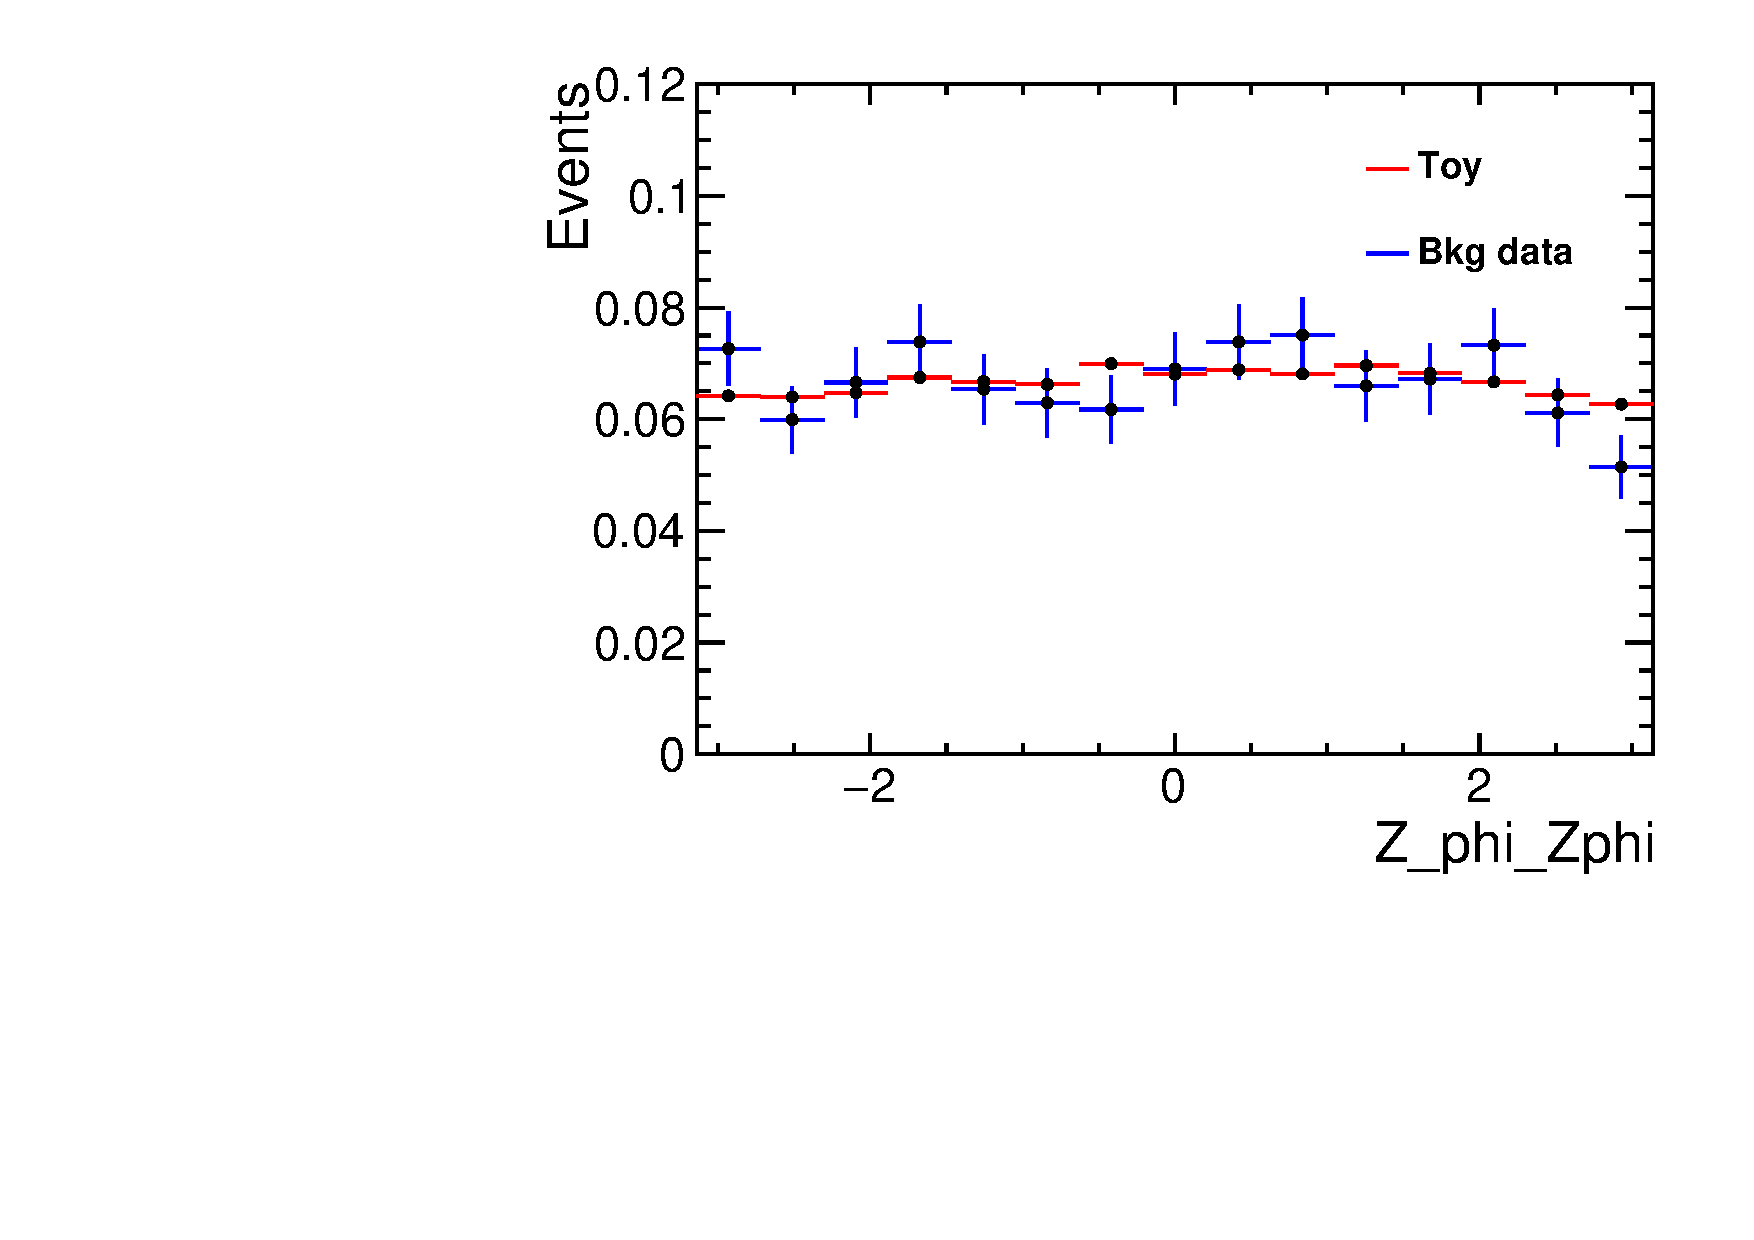
\includegraphics[width=0.3\textwidth]{Figures/03_Zcs/app_sideband/Z_phi_Zphi.pdf}\\
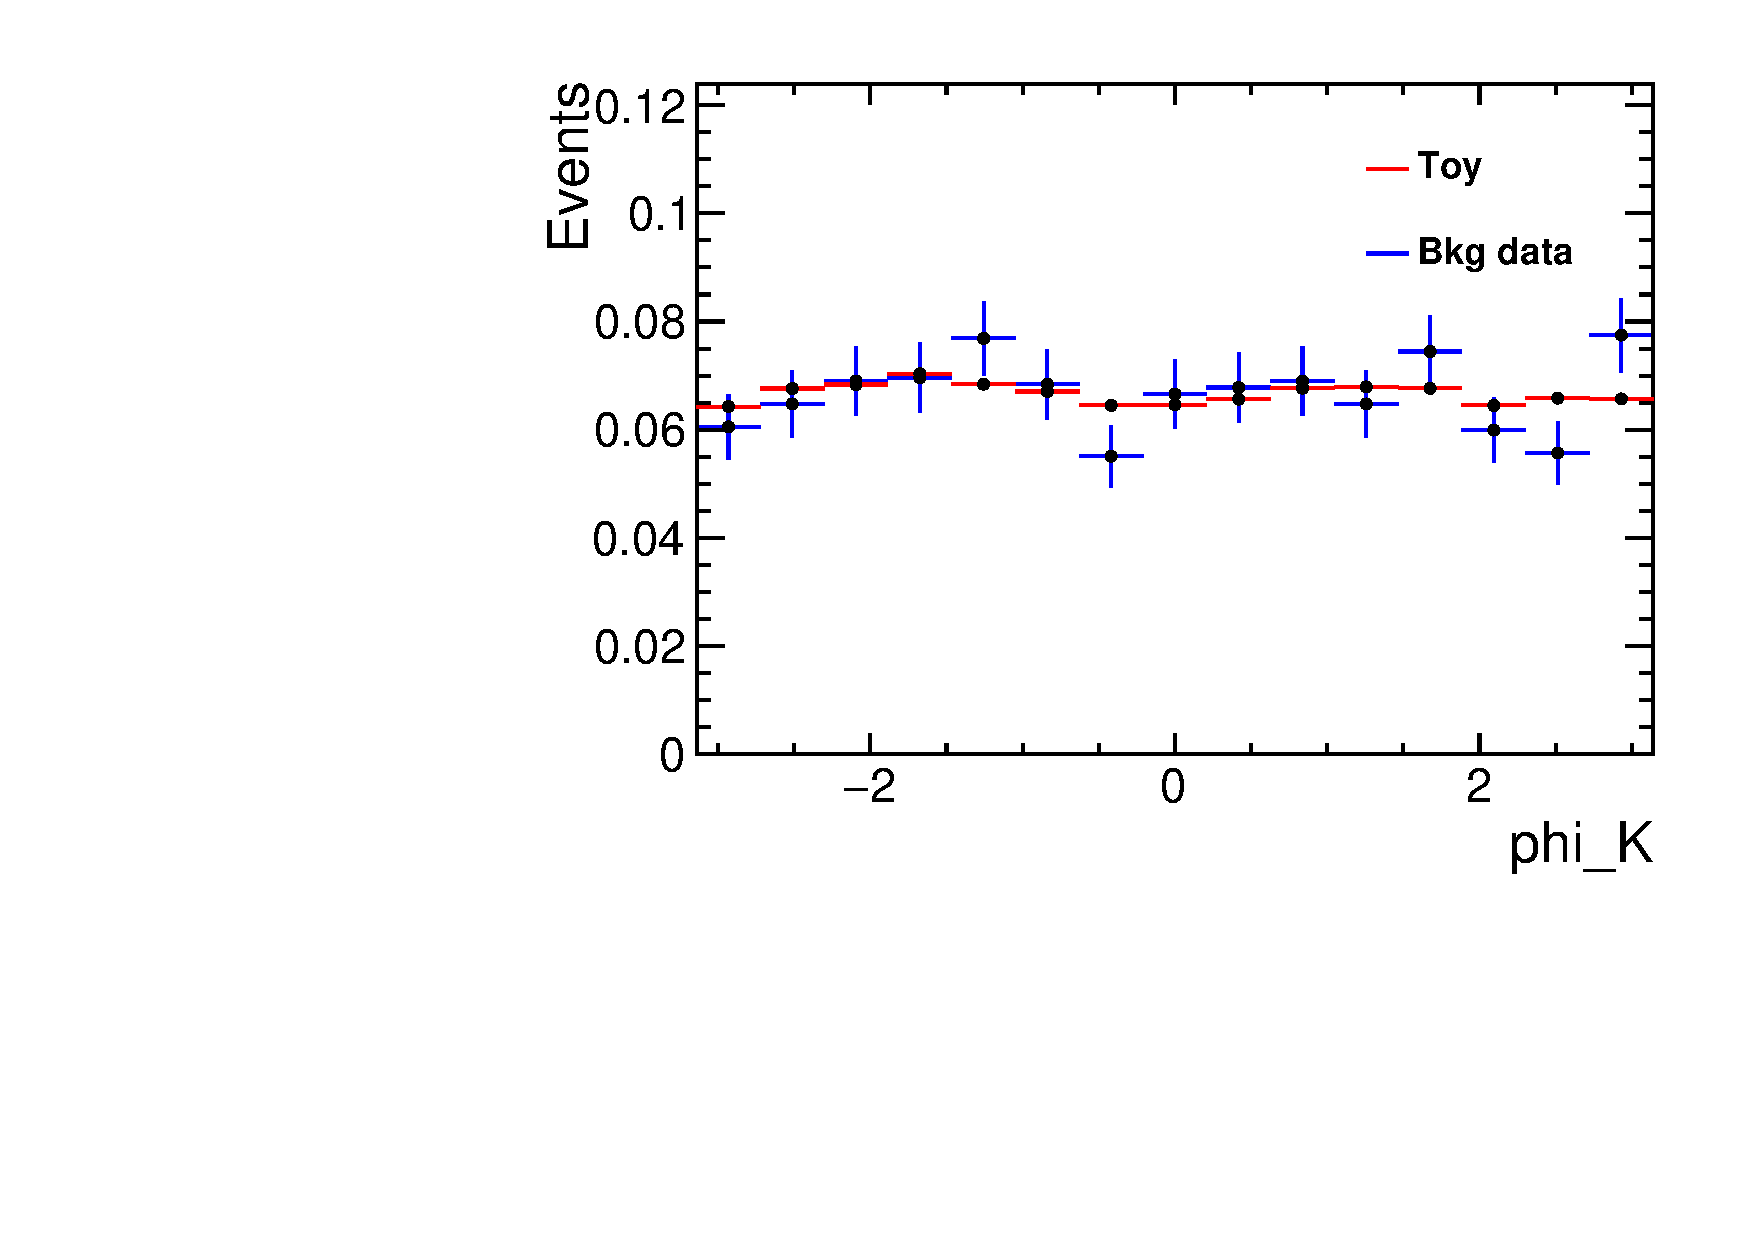
\includegraphics[width=0.3\textwidth]{Figures/03_Zcs/app_sideband/phi_K.pdf} %
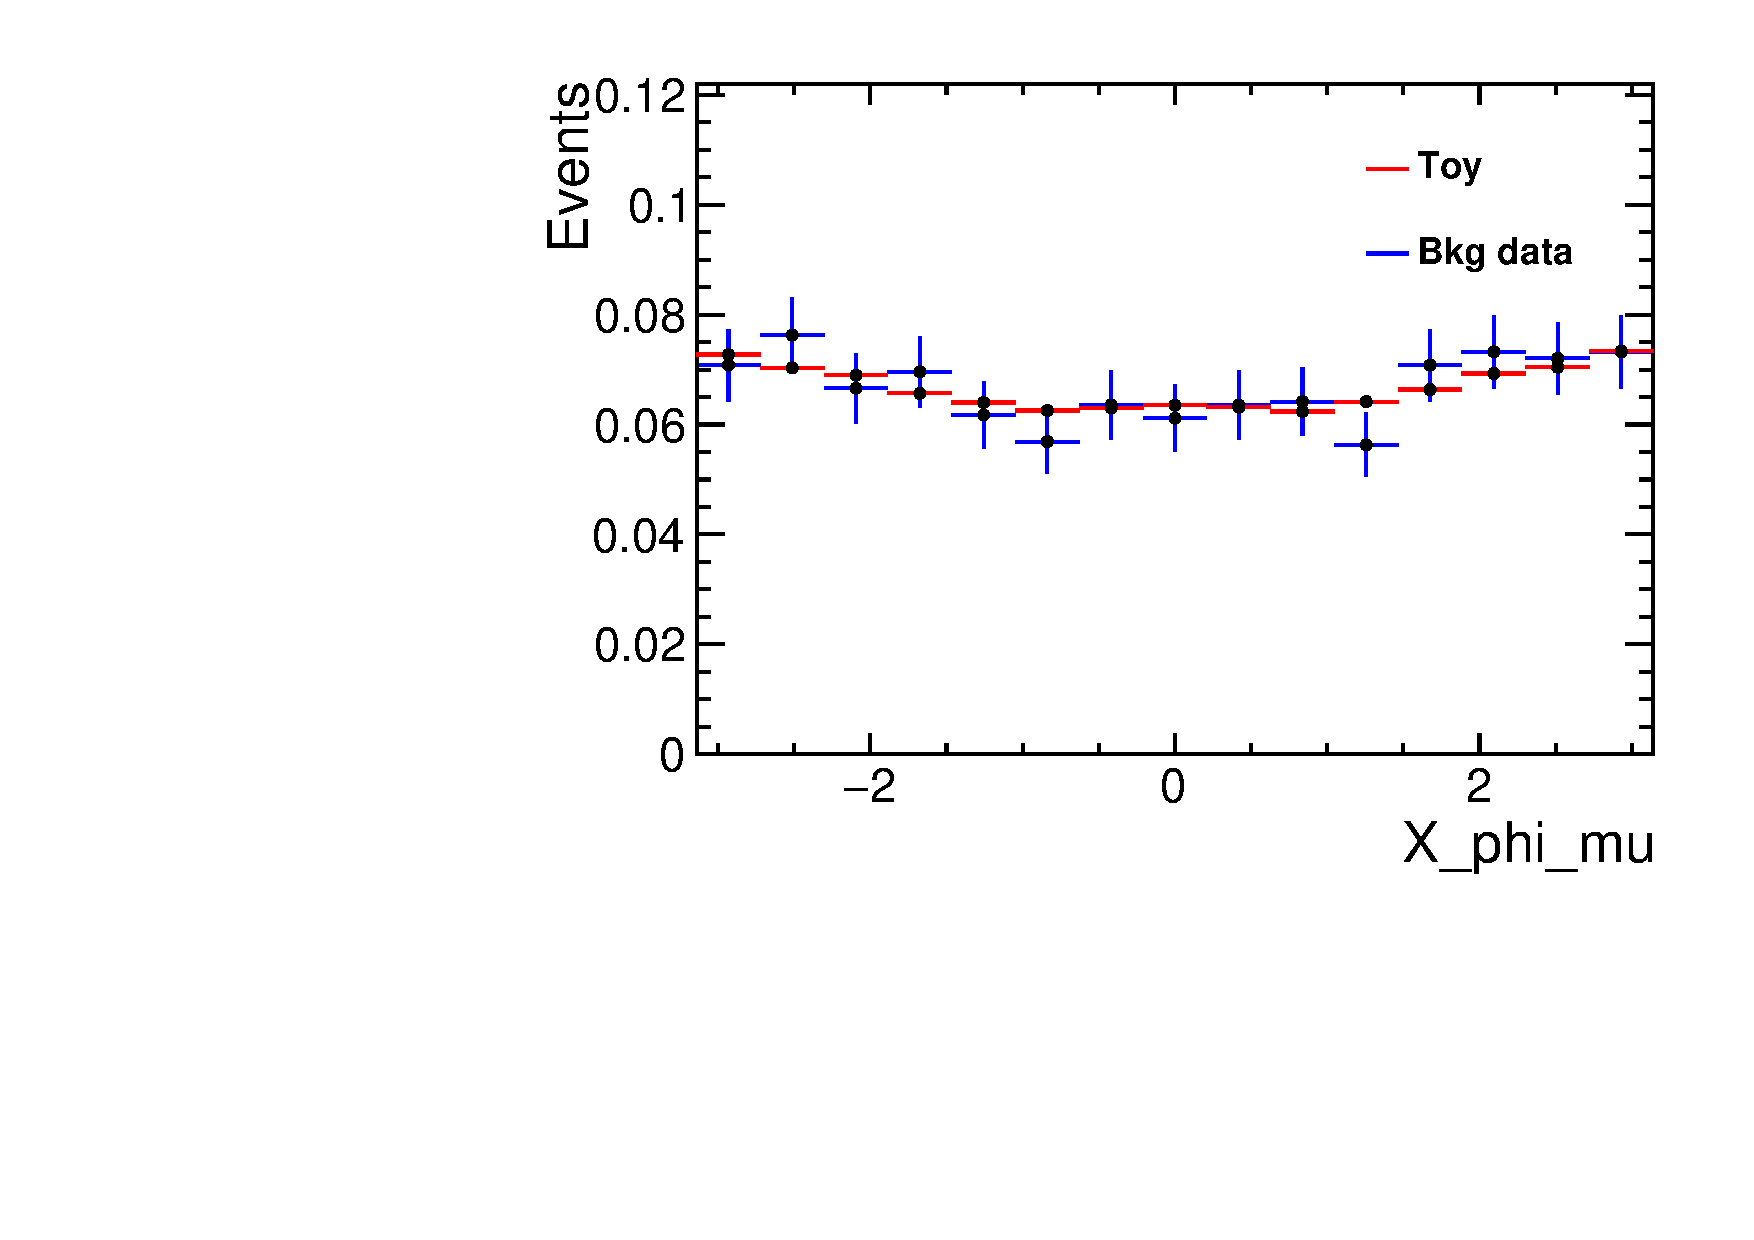
\includegraphics[width=0.3\textwidth]{Figures/03_Zcs/app_sideband/X_phi_mu.pdf} %
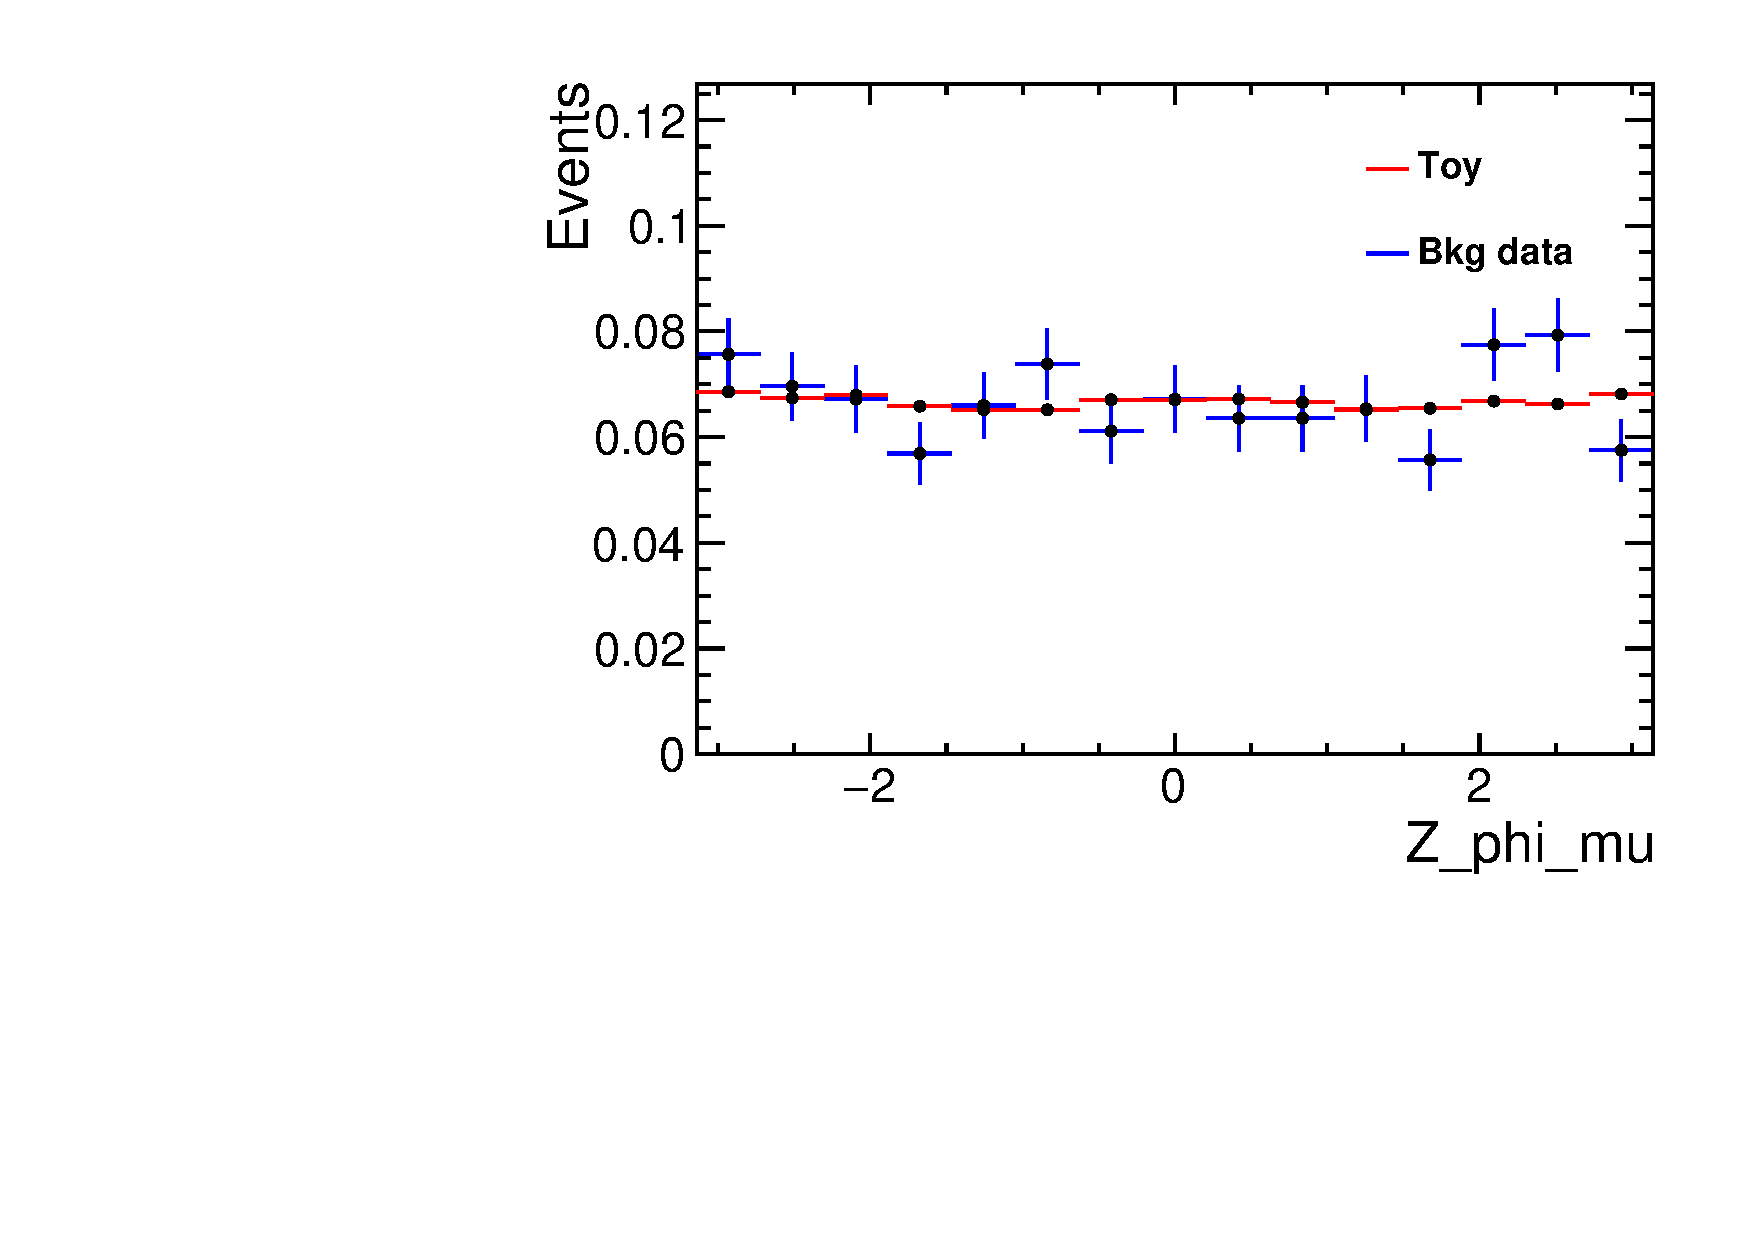
\includegraphics[width=0.3\textwidth]{Figures/03_Zcs/app_sideband/Z_phi_mu.pdf}% \\
\caption{Comparison between the parametrized background PDF used in the default cFit (red dots) with the $B$ sideband data (blue dots) for all masses and angles used in nominal fit, for $K^*$ chain (left) $X$ chain (middle) and $Z_{cs}$ chain (right).}
\label{fig:mass_distribution_phi_sideband}
\end{figure}


Among the systematic variations we include an alternative way to
parameterize the background PDF. Instead of assuming factorization, we use decomposition of the background density and of the efficiency into their multidimensional moments in the $K^*$ decay chain variables. For examples, the efficiency parametrization becomes:
\begin{eqnarray}
\epsilon(\mfk,\Omega) &=& \sum_{a,b,c,d,e,f}\epsilon^{abcdef}{\cal{P}}_a(\cos\theta_{K^*})Y_{bc}(\cos\theta_{\psi},\phi_{(\psi K^*)})\nonumber\\
&& \quad \quad \times {\cal{P}}_d\left(2\frac{\mfk-\mfk^{\rm min}}{\mfk^{\rm max}-\mfk^{\rm min}}-1\right) {\cal{P}}_e(\cos\theta_{\phi}){\cal{P}}_f(\frac{\phi_\Kp}{\pi}),
\end{eqnarray}\label{EqEff}
where ${\cal{P}}$ is Legendre polynomial, $Y_{bc}$ are spherical harmonics, and $\mfk^{\rm min}$ and $\mfk^{\rm max}$ are the minimum and maximum allowed values for $\mfk$, respectively. The $Y_{bc}$ functions are complex functions. To ensure that the efficiency function is real, we set $\epsilon^{abcdef}=-\epsilon^{ab(-c)def}$. The values of $\epsilon^{abcdef}$ are determined by summing over the fully simulated phase-space events or sideband events
\begin{eqnarray}\label{eq:effco}
\epsilon^{abcdef}&=&\frac{1}{\sum_i w_i}\sum_i w_i \frac{2a+1}{2}\frac{2d+1}{2} \frac{2e+1}{2}\frac{2f+1}{2}{\cal{P}}_a(\cos\theta_{K^*},i)Y_{bc}(\cos\theta_{\psi,i},\phi_{(\psi K^*),i})\nonumber\\
&&\quad \quad \times {\cal{P}}_d\left(2\frac{m_{\phi K,i}-\mfk^{\rm min}}{\mfk^{\rm max}-\mfk^{\rm min}}-1\right) {\cal{P}}_e(\cos\theta_{\phi,i}){\cal{P}}_f(\frac{\phi_{\Kp,i}}{\pi})\frac{1}{g_i},
\end{eqnarray}
where the weights $w^{\rm mc}_i$ account for GB weights for $\Bp$ $p$ , $\pt$ and multiplicity (for background $w_i^{\rm bkg}=1$, and $g_i$ is the value of the phase-space probability density for event $i$). This approach allows the description of multidimensional correlations without assuming factorization. In practice, the sum is over a finite number of terms ($a\leq10$, $b\leq4$, $-2\leq c\leq2$, $d,e,f\leq8$) and only coefficients with a statistical significance larger than three standard deviations $(\sigma)$ from zero are retained. The fit results obtained with this approach are included in the tables of systematic errors in Sec.~\ref{sec:sys}.
We also show comparison of this paramaterization to the sideband data in Fig.~\ref{fig:mass_distribution_phi_sideband_2}.



\begin{figure}[!hbtp]
\centering
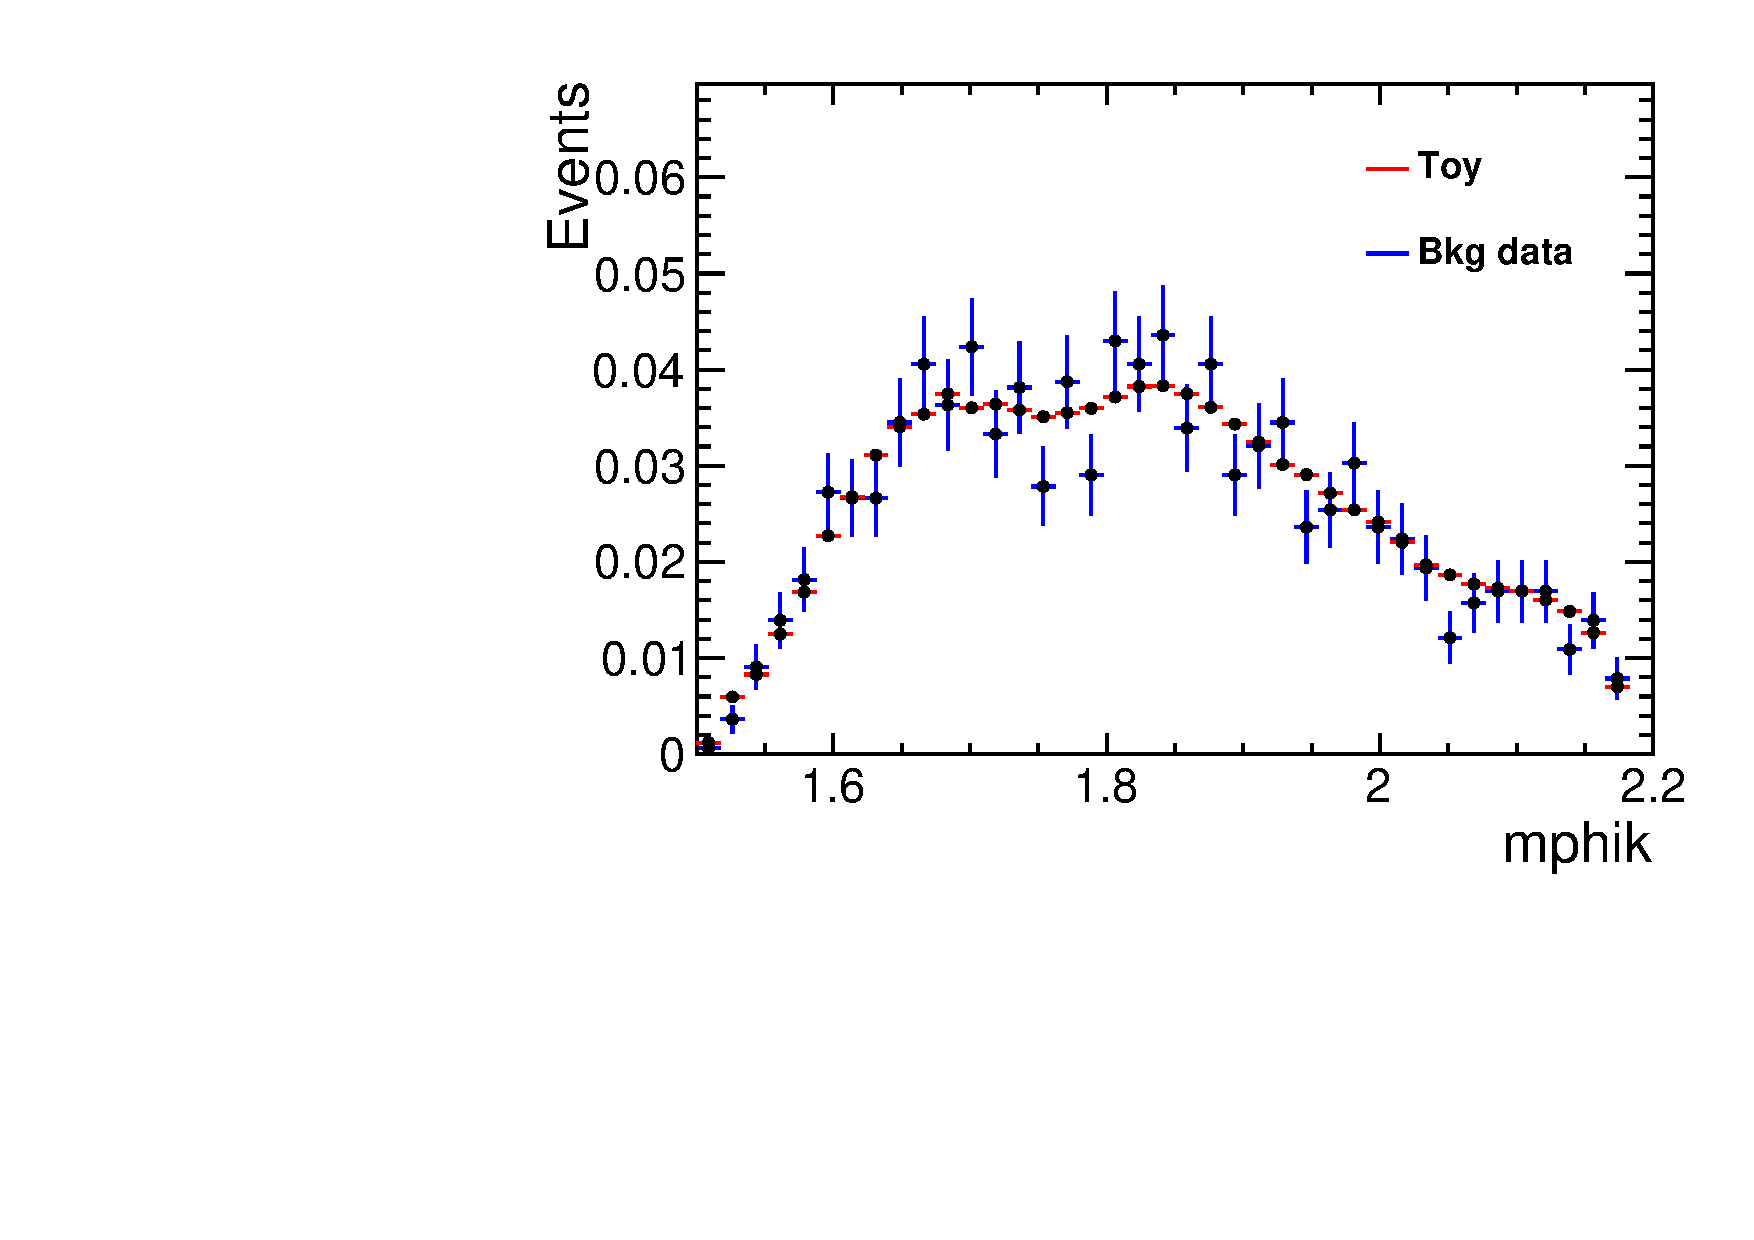
\includegraphics[width=0.3\textwidth]{Figures/03_Zcs/app_sideband/mphik.pdf}  %
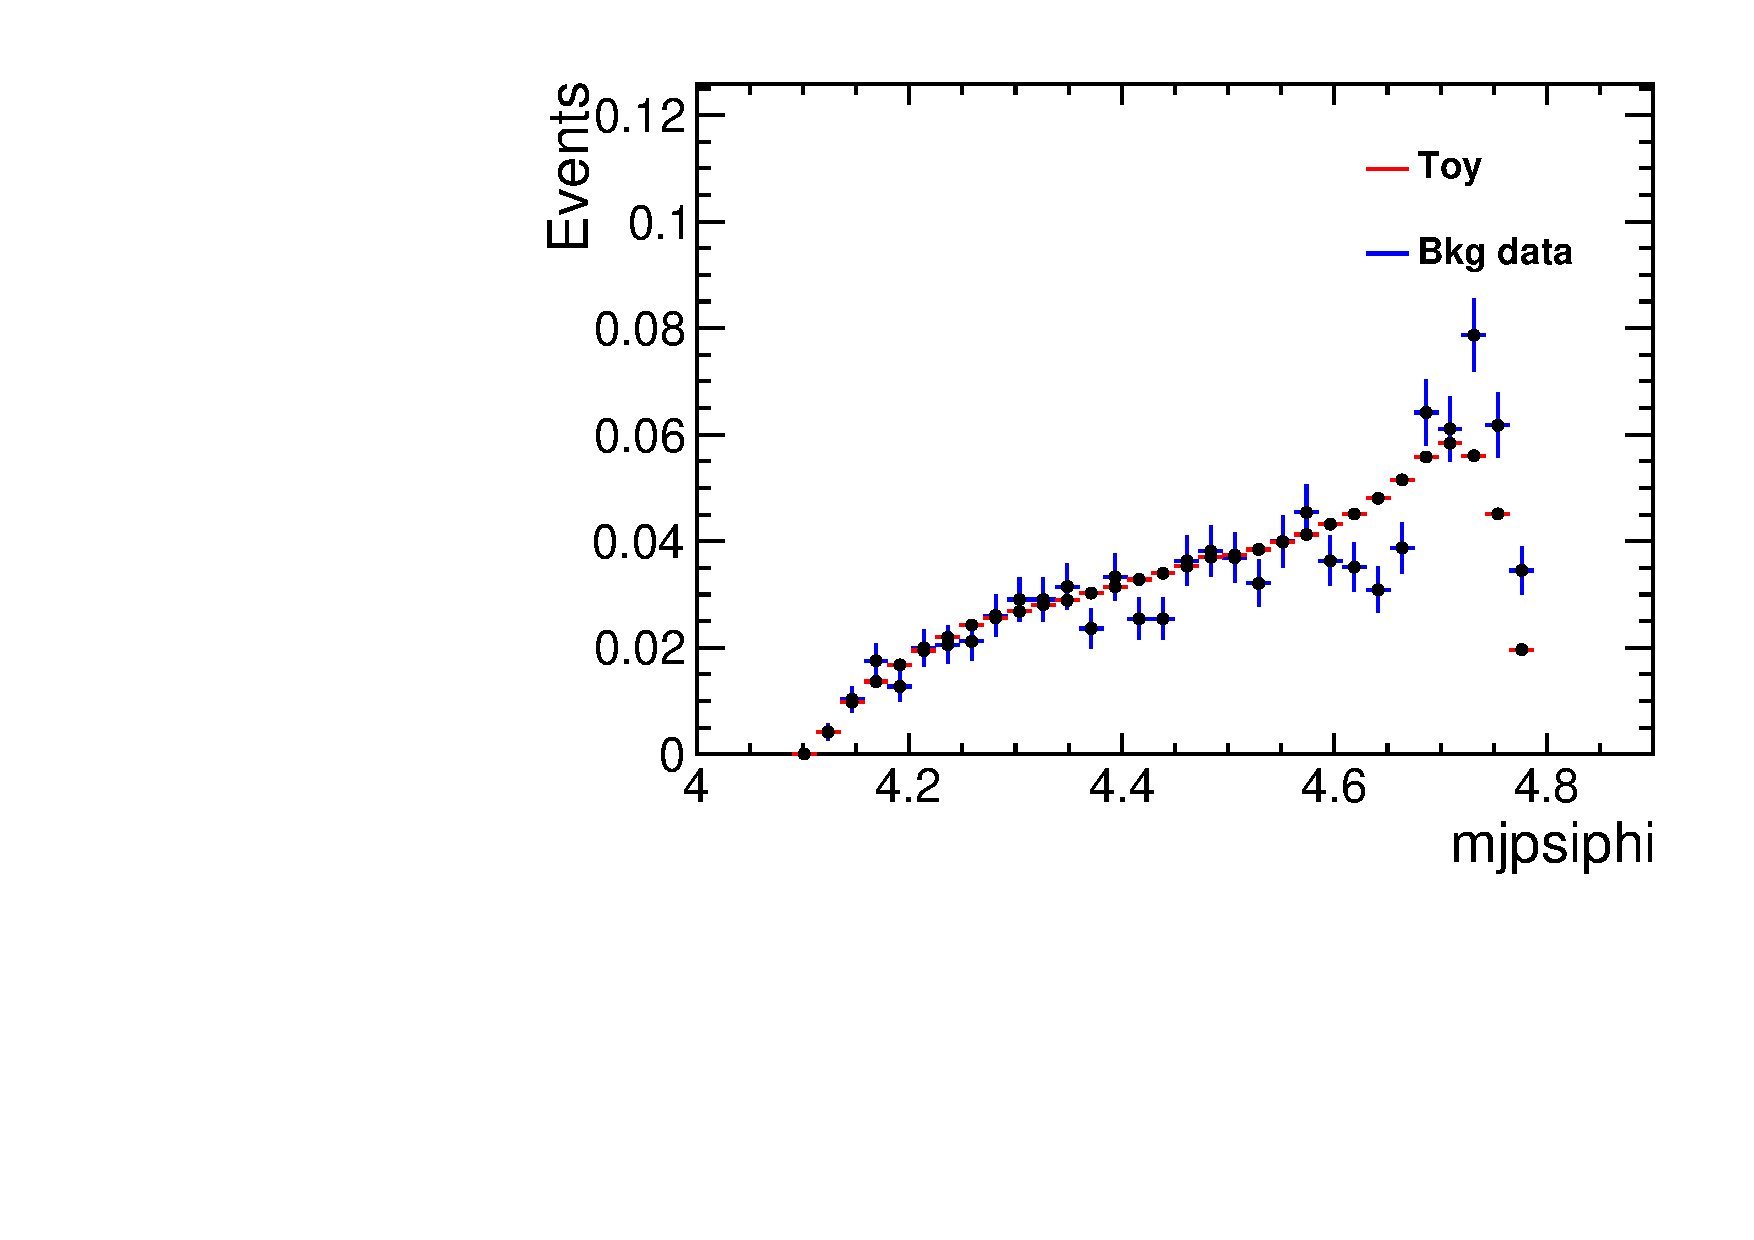
\includegraphics[width=0.3\textwidth]{Figures/03_Zcs/app_sideband/mjpsiphi.pdf}  %
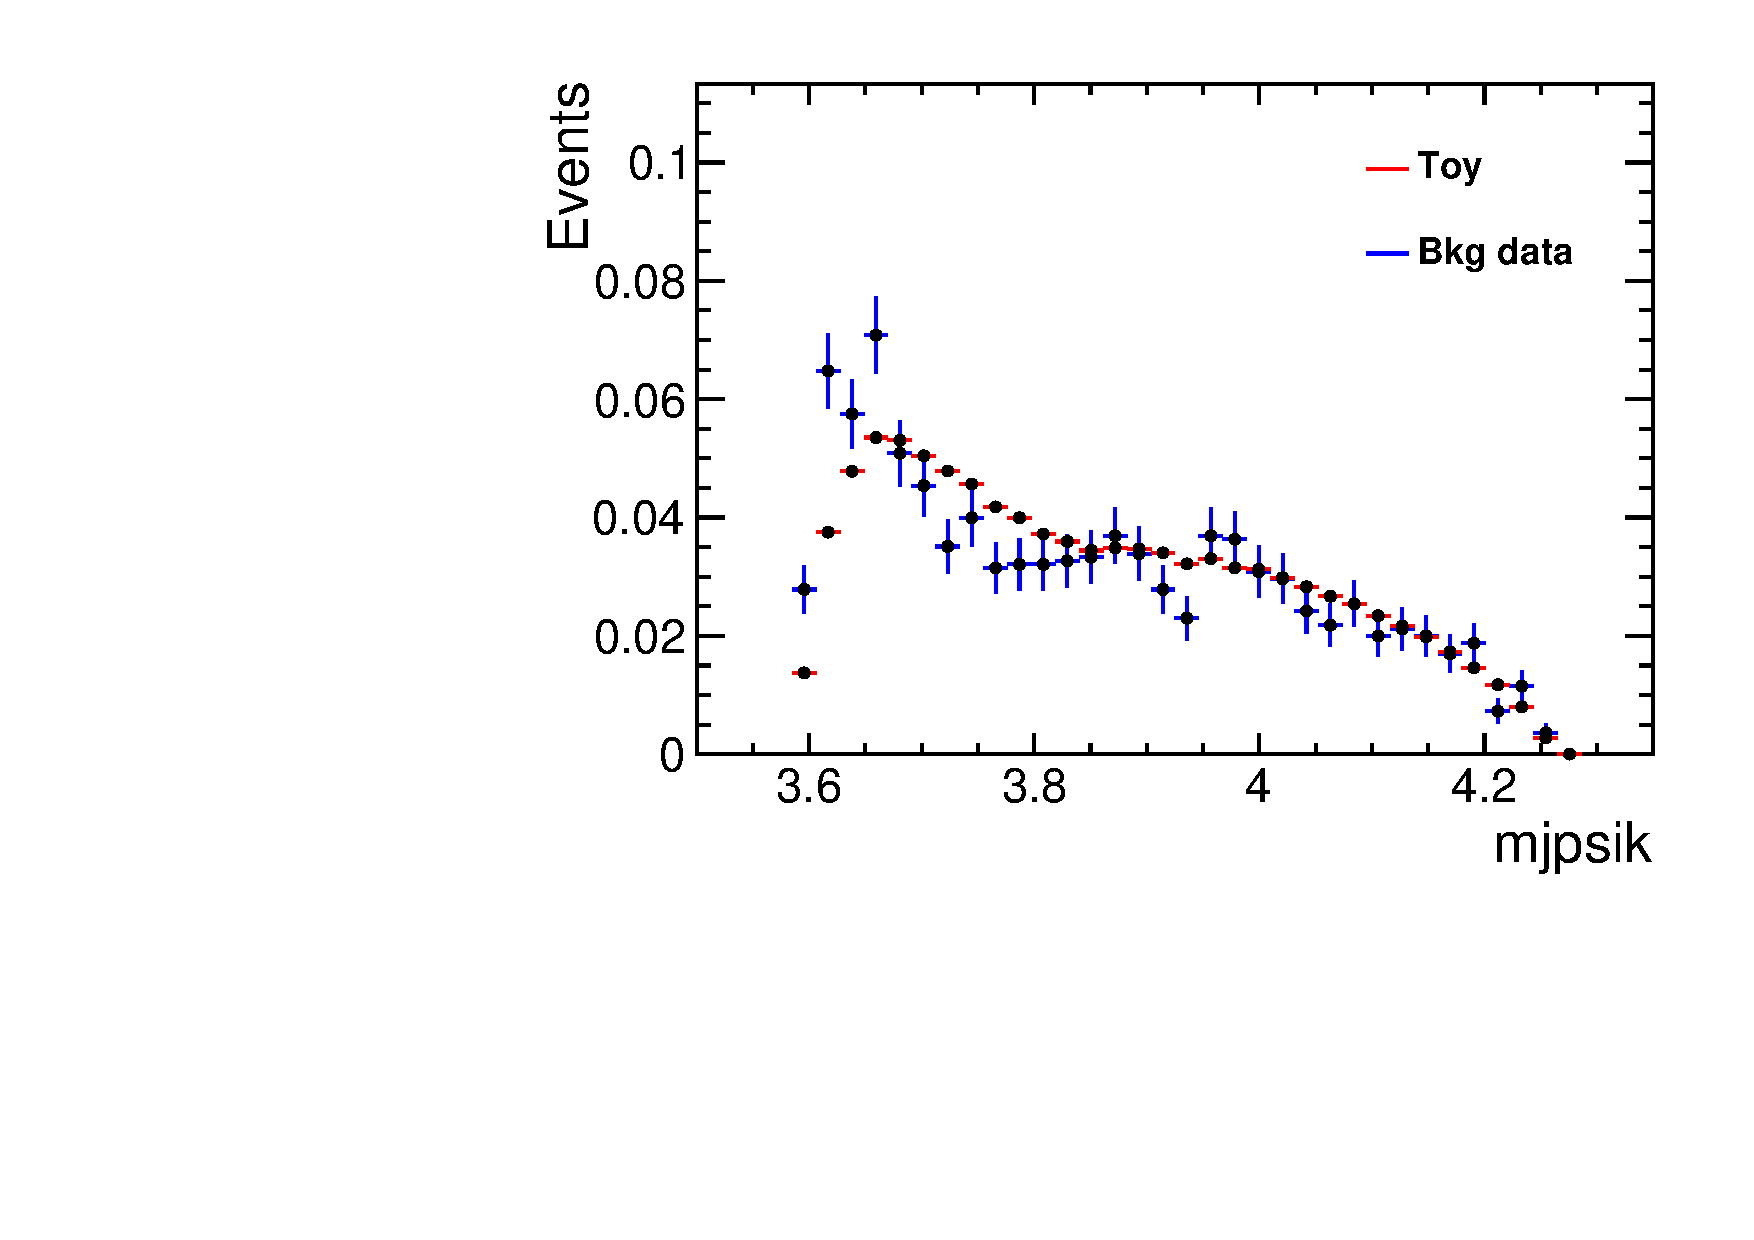
\includegraphics[width=0.3\textwidth]{Figures/03_Zcs/app_sideband/mjpsik.pdf} \\
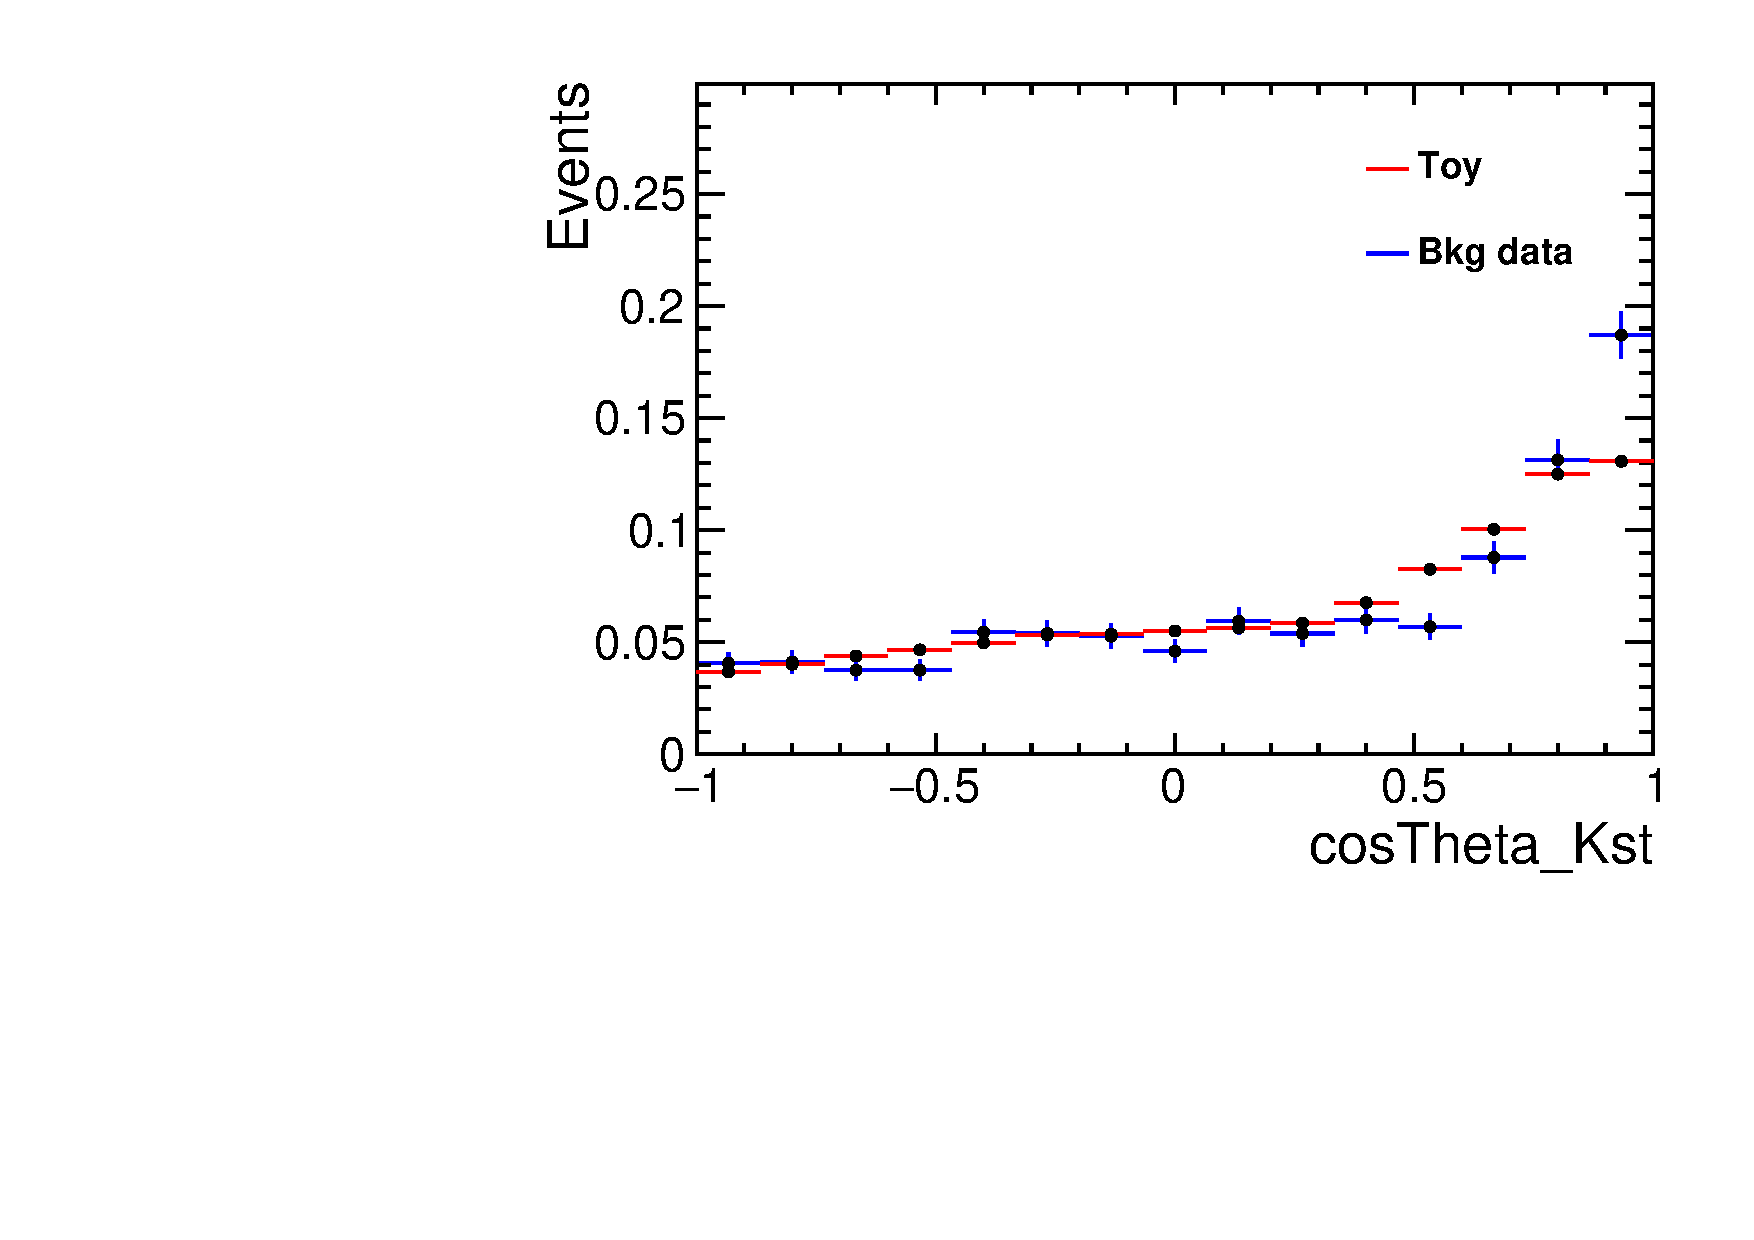
\includegraphics[width=0.3\textwidth]{Figures/03_Zcs/app_sideband/cosTheta_Kst.pdf}%
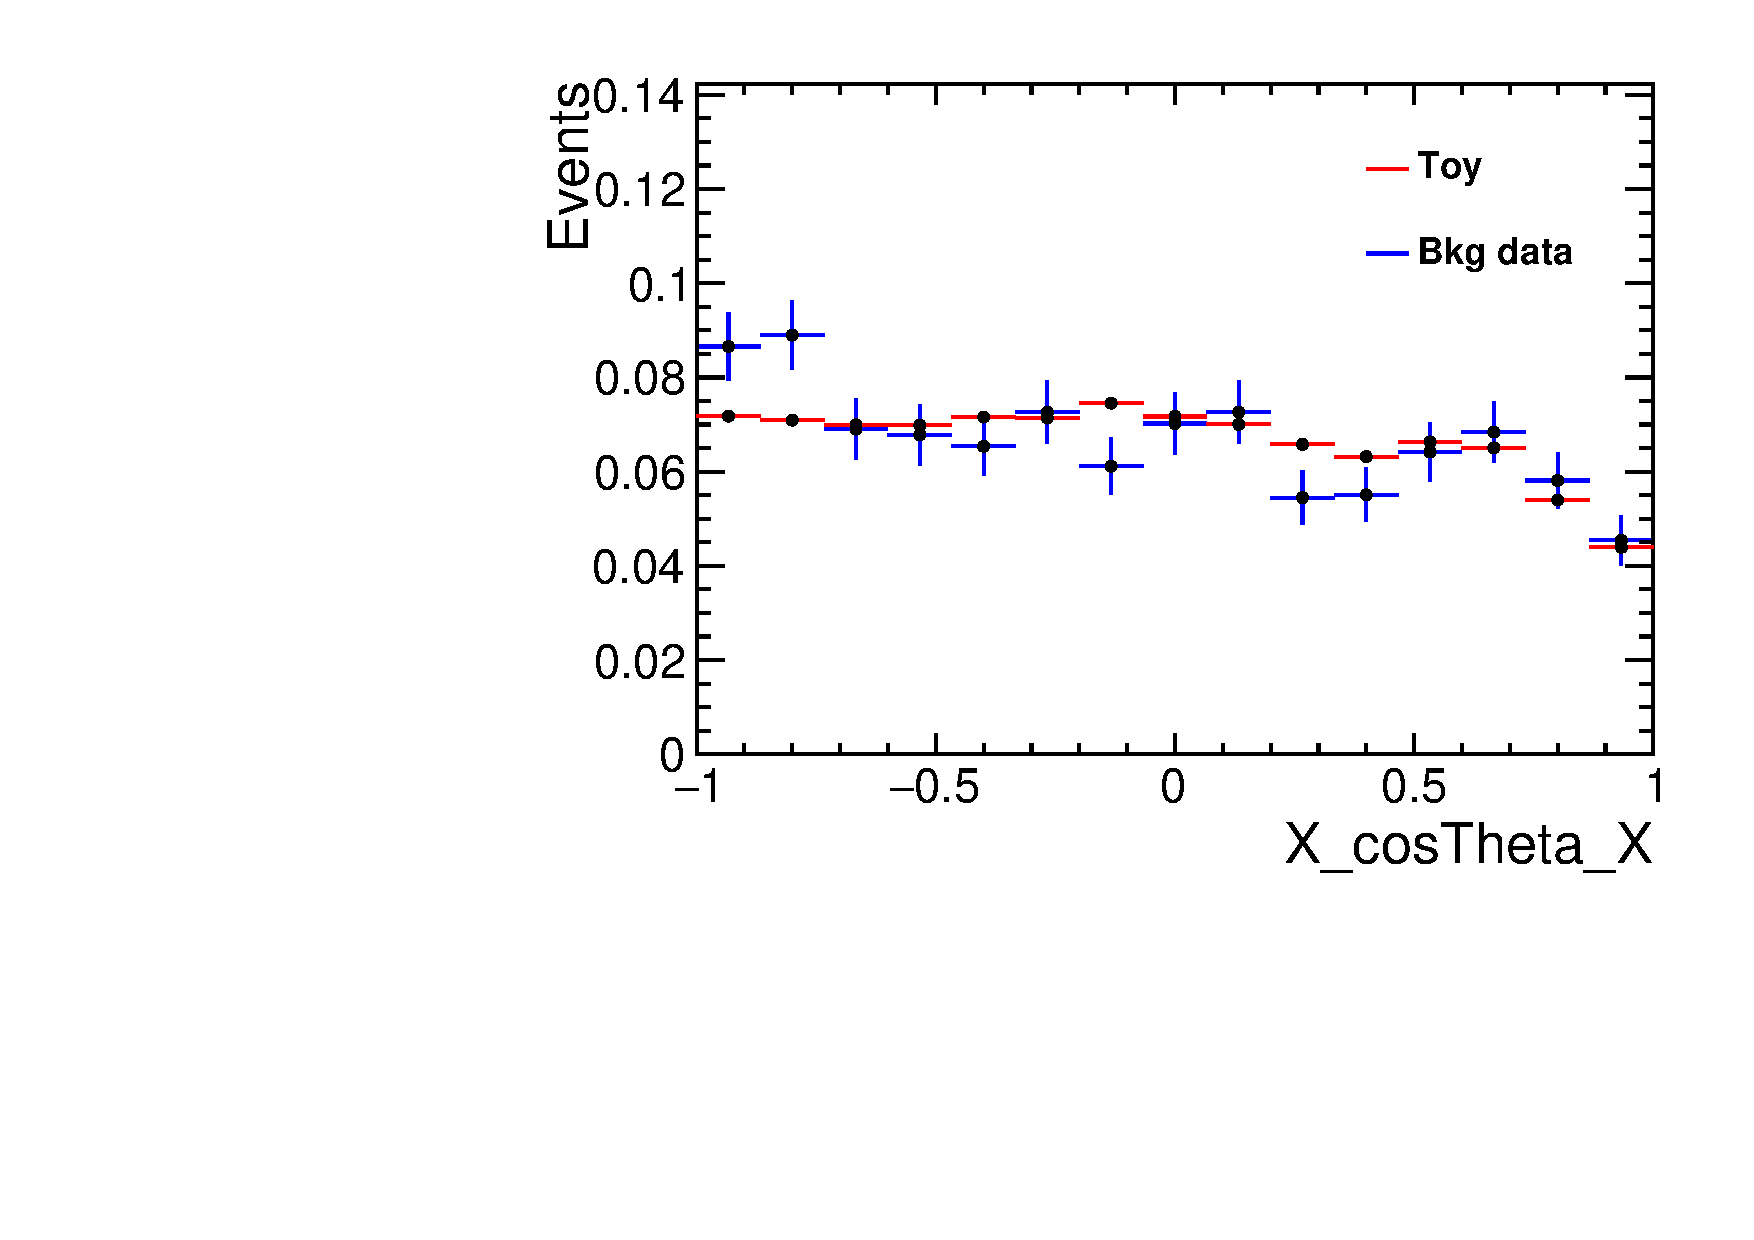
\includegraphics[width=0.3\textwidth]{Figures/03_Zcs/app_sideband/X_cosTheta_X.pdf}%
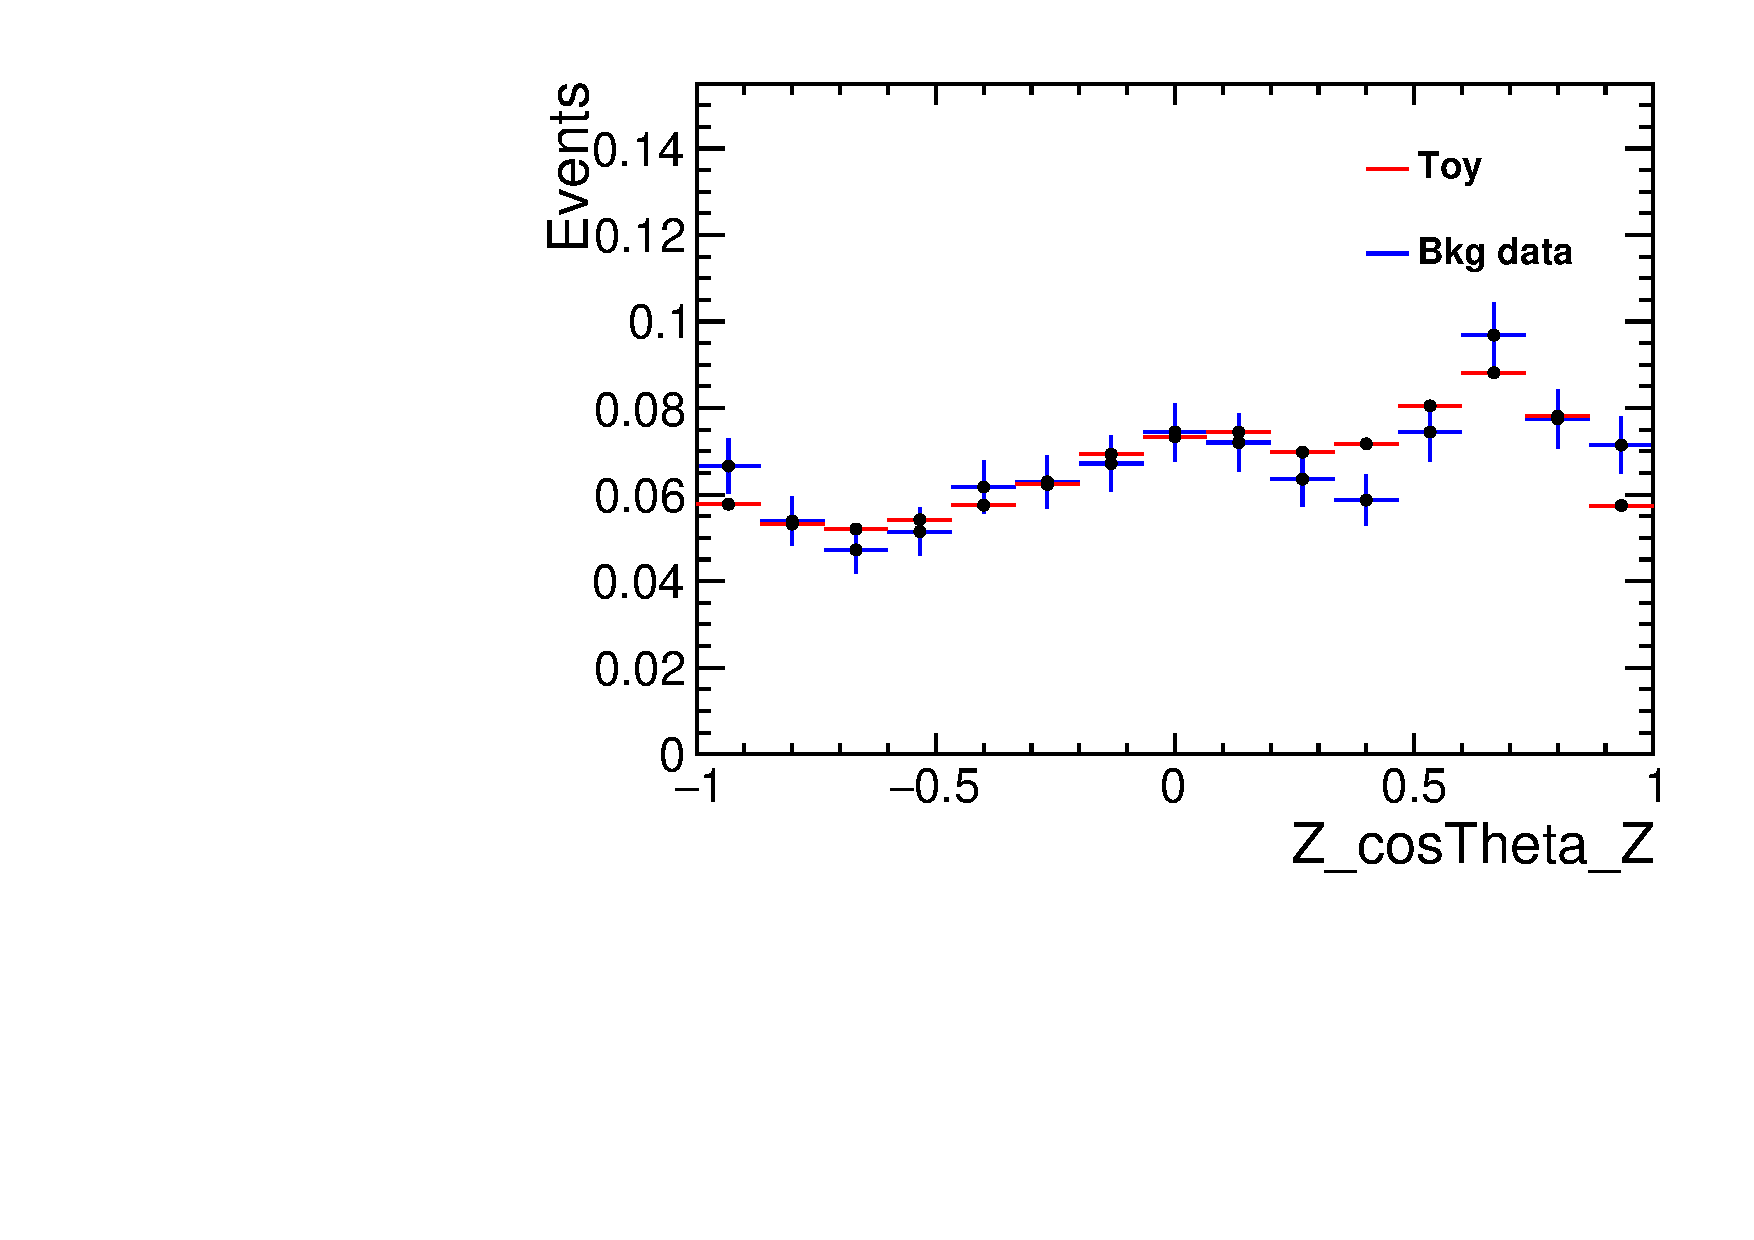
\includegraphics[width=0.3\textwidth]{Figures/03_Zcs/app_sideband/Z_cosTheta_Z.pdf} \\%
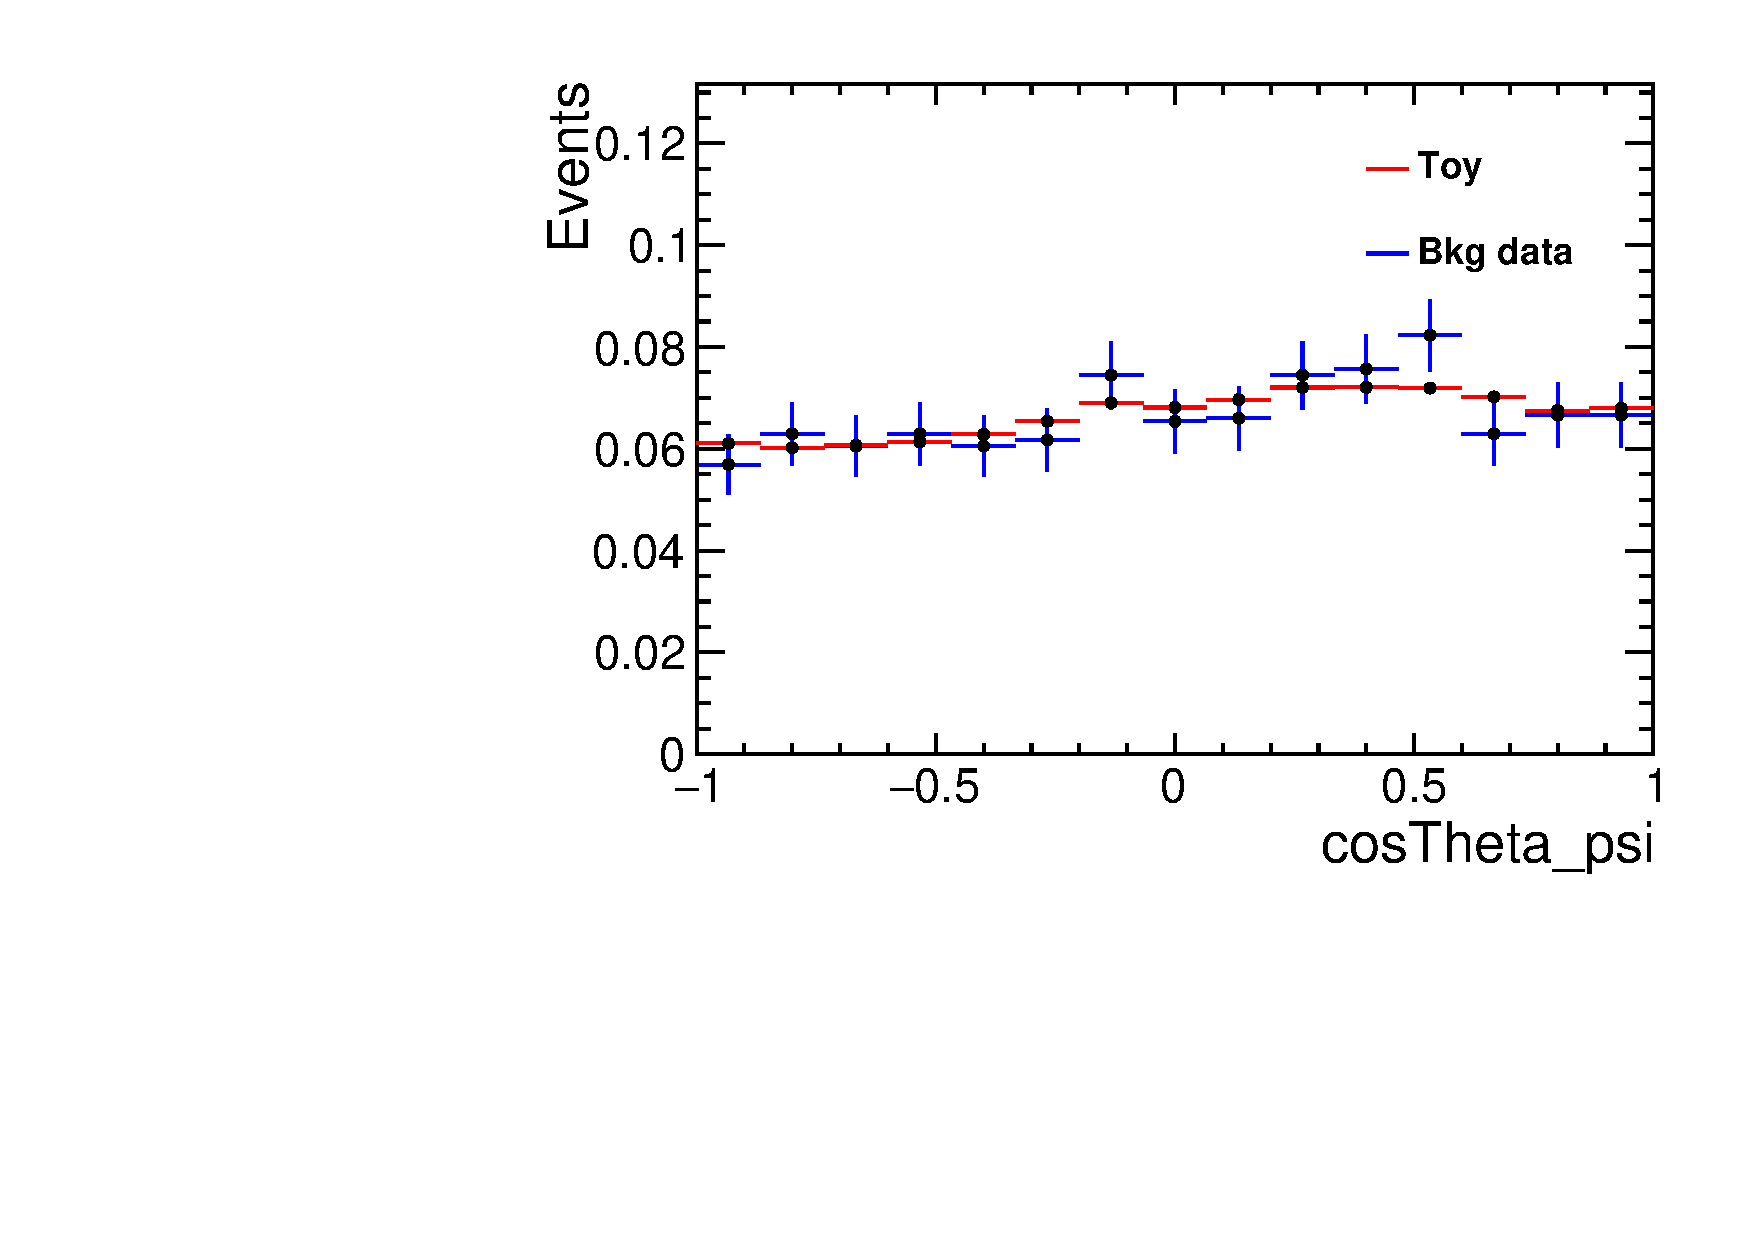
\includegraphics[width=0.3\textwidth]{Figures/03_Zcs/app_sideband/cosTheta_psi.pdf}%
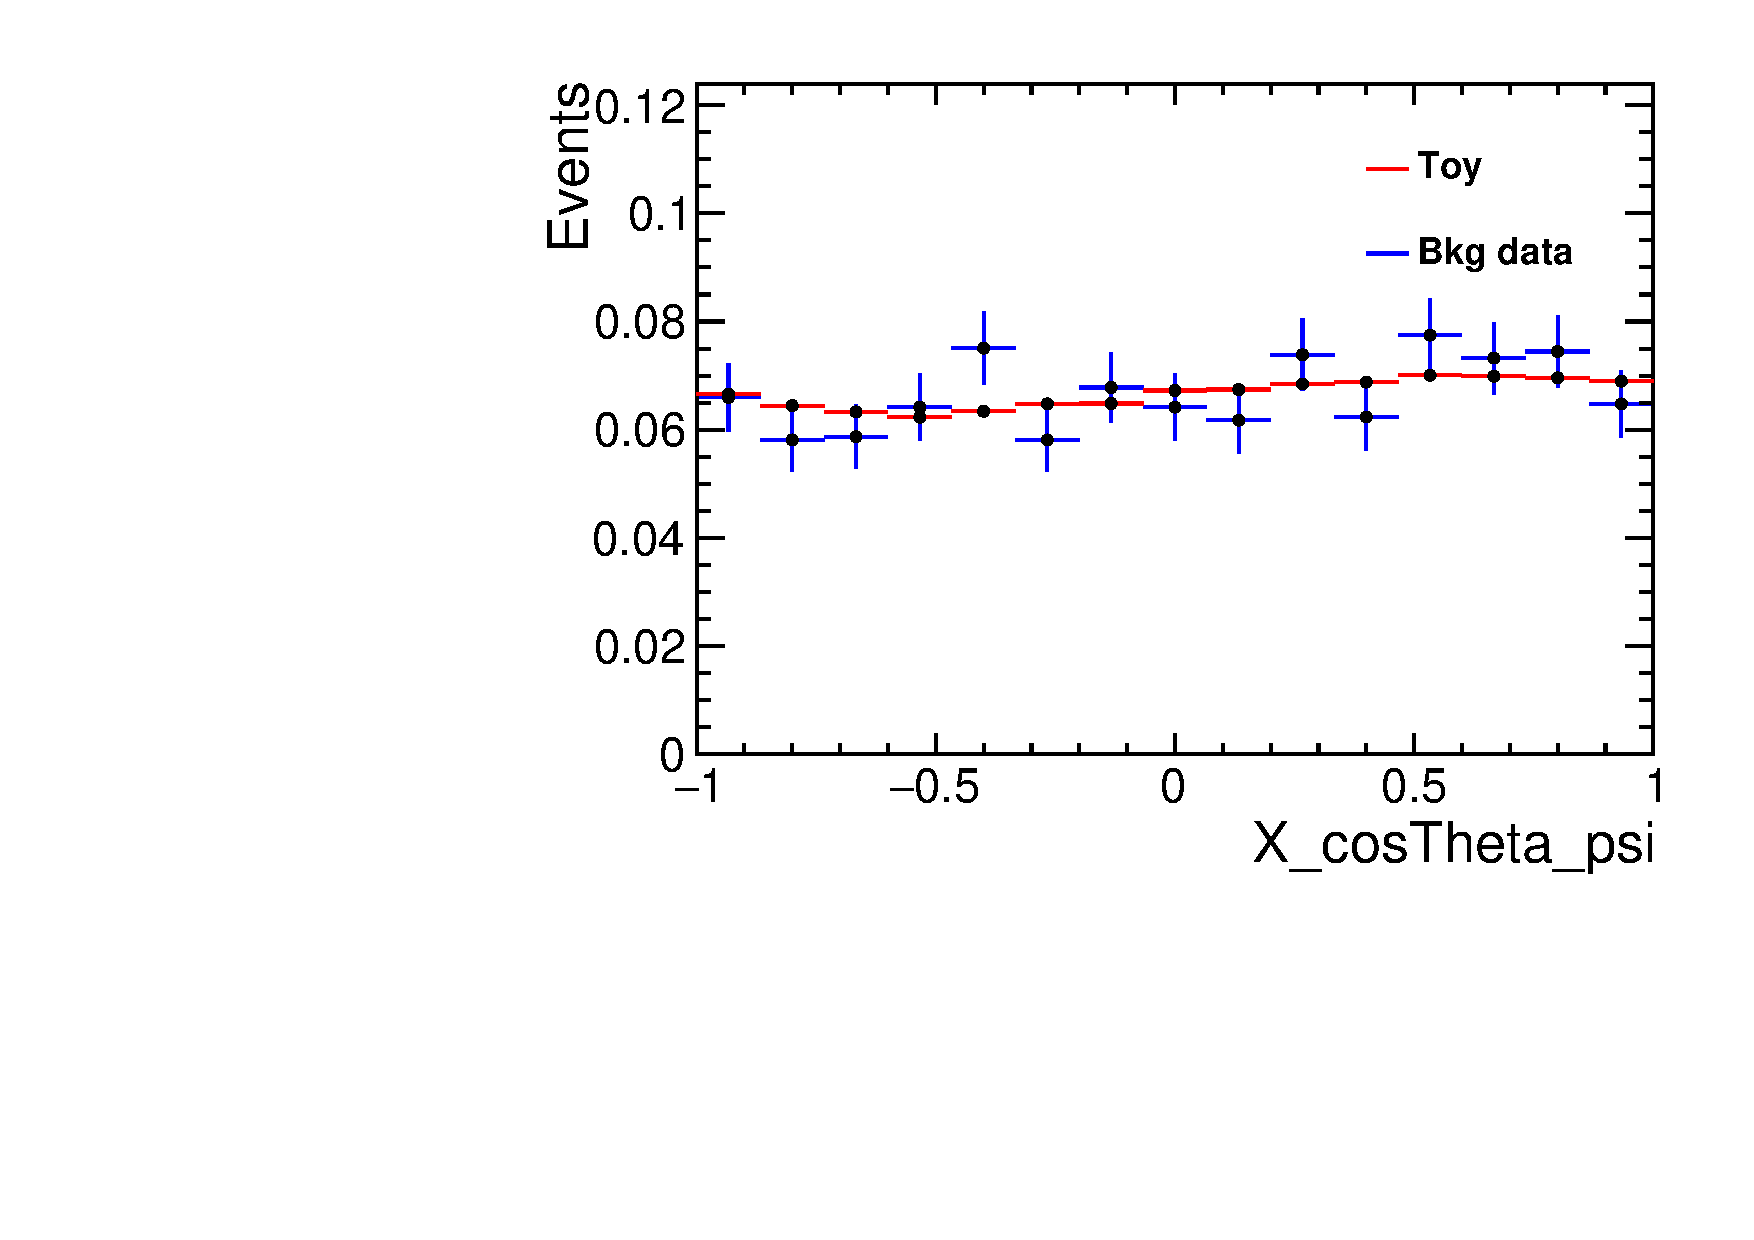
\includegraphics[width=0.3\textwidth]{Figures/03_Zcs/app_sideband/X_cosTheta_psi.pdf}%
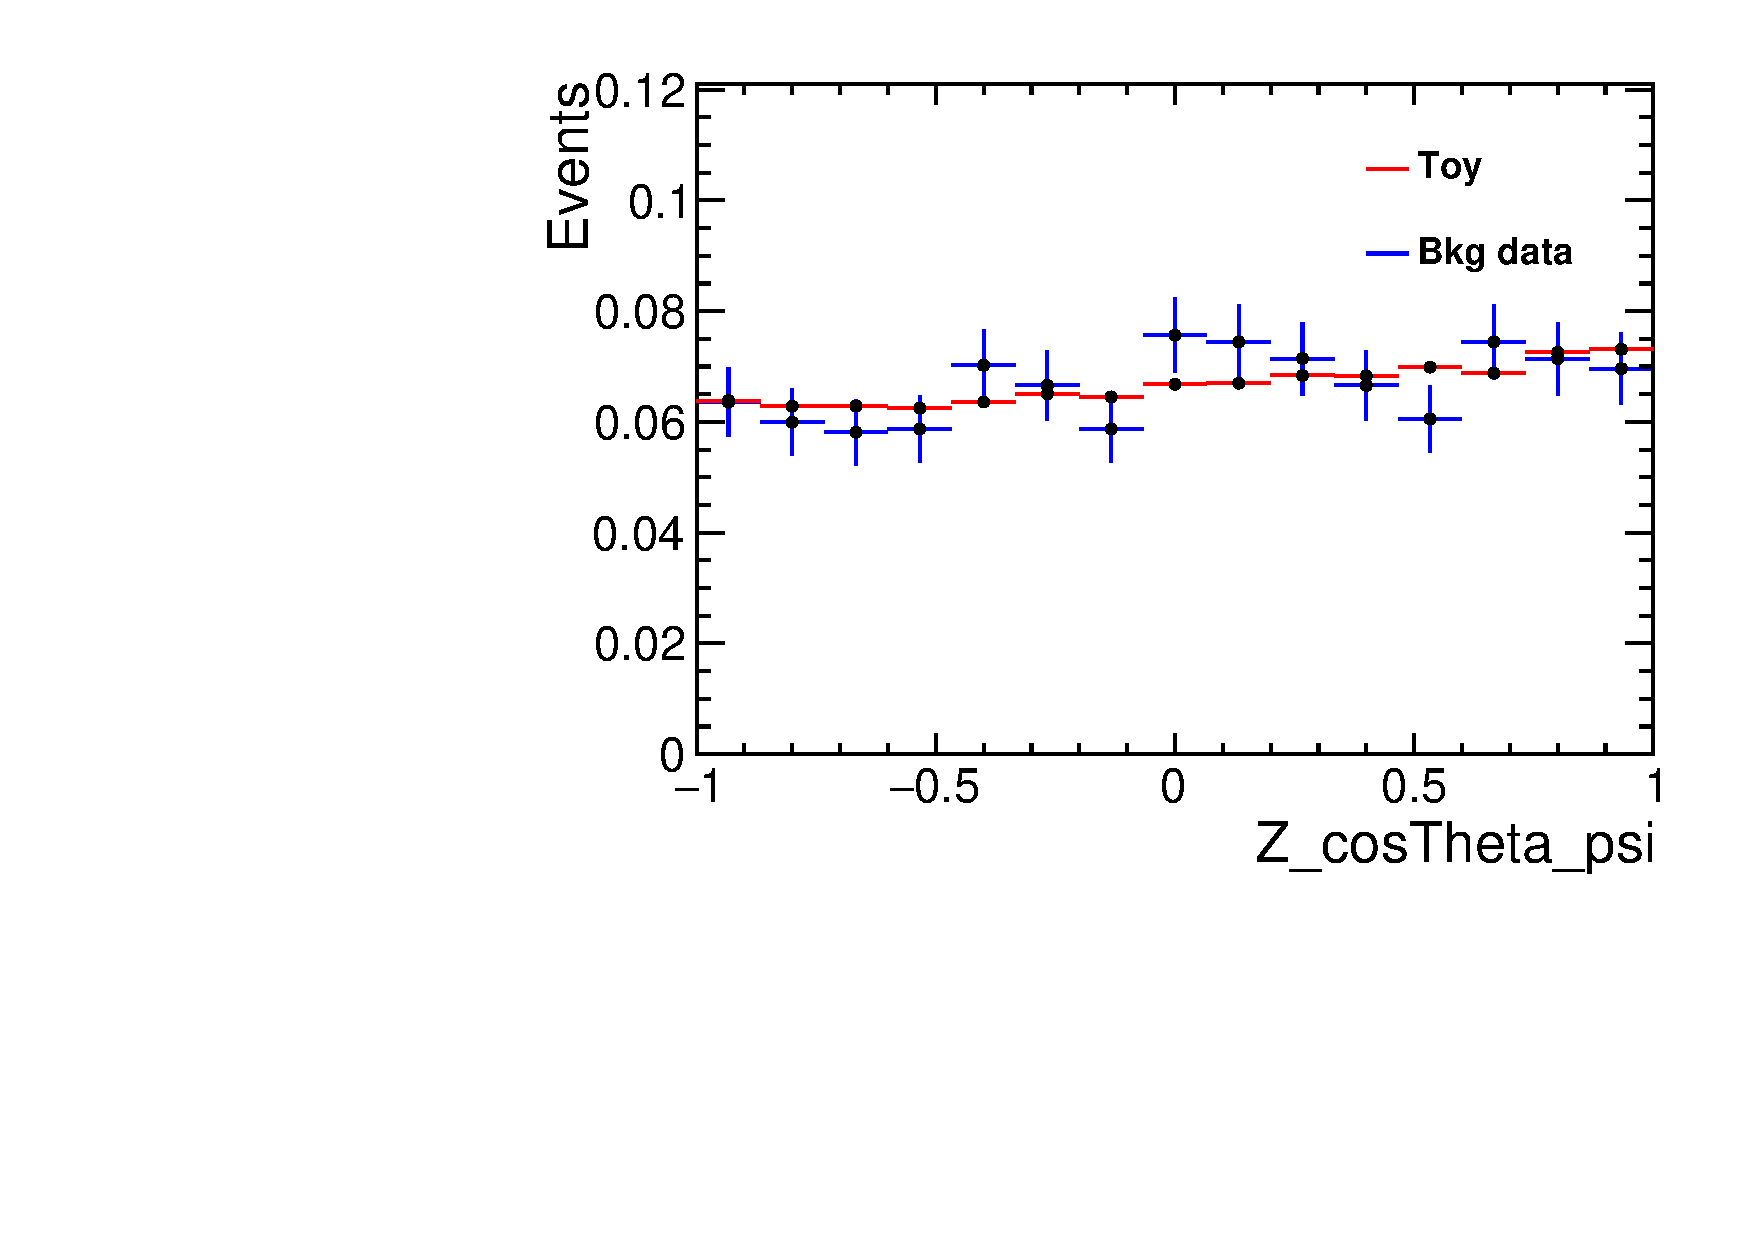
\includegraphics[width=0.3\textwidth]{Figures/03_Zcs/app_sideband/Z_cosTheta_psi.pdf}\\
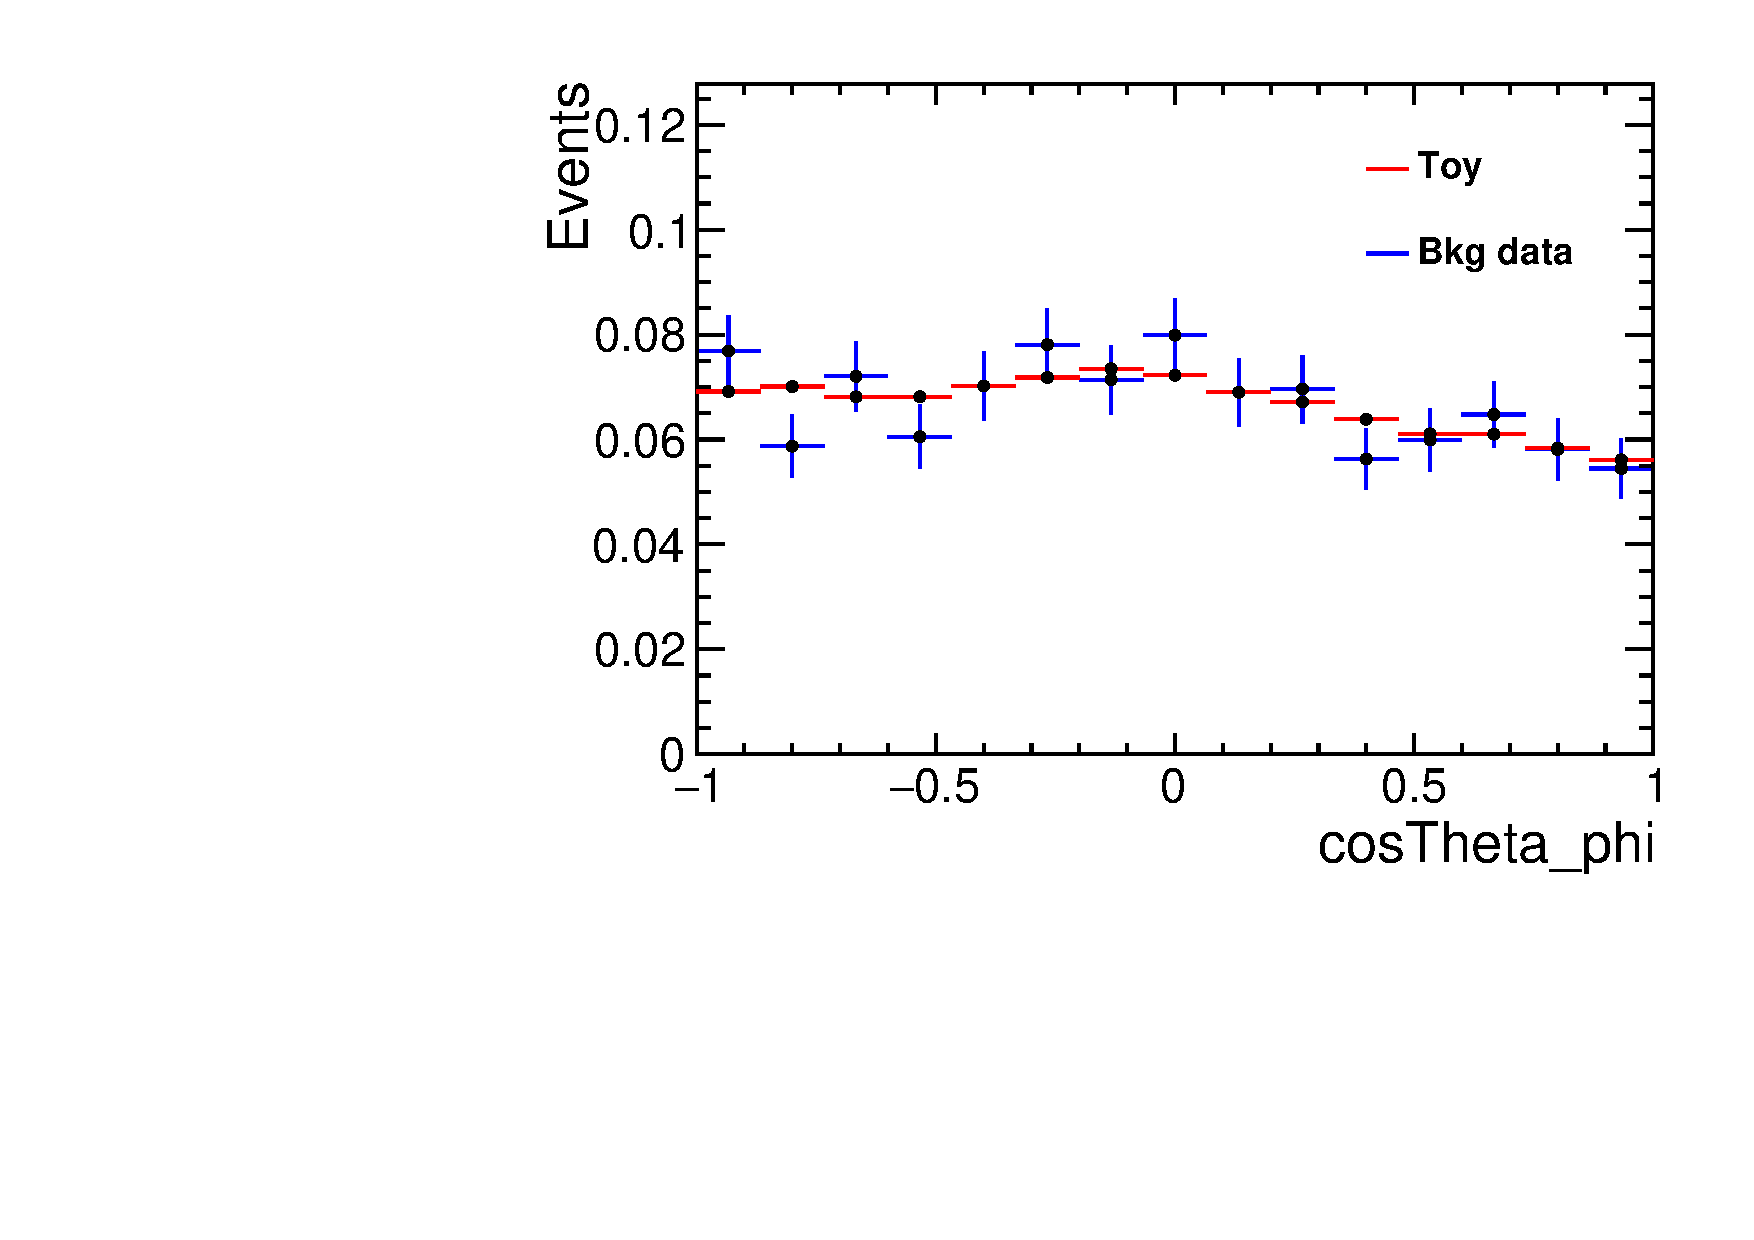
\includegraphics[width=0.3\textwidth]{Figures/03_Zcs/app_sideband/cosTheta_phi.pdf}%
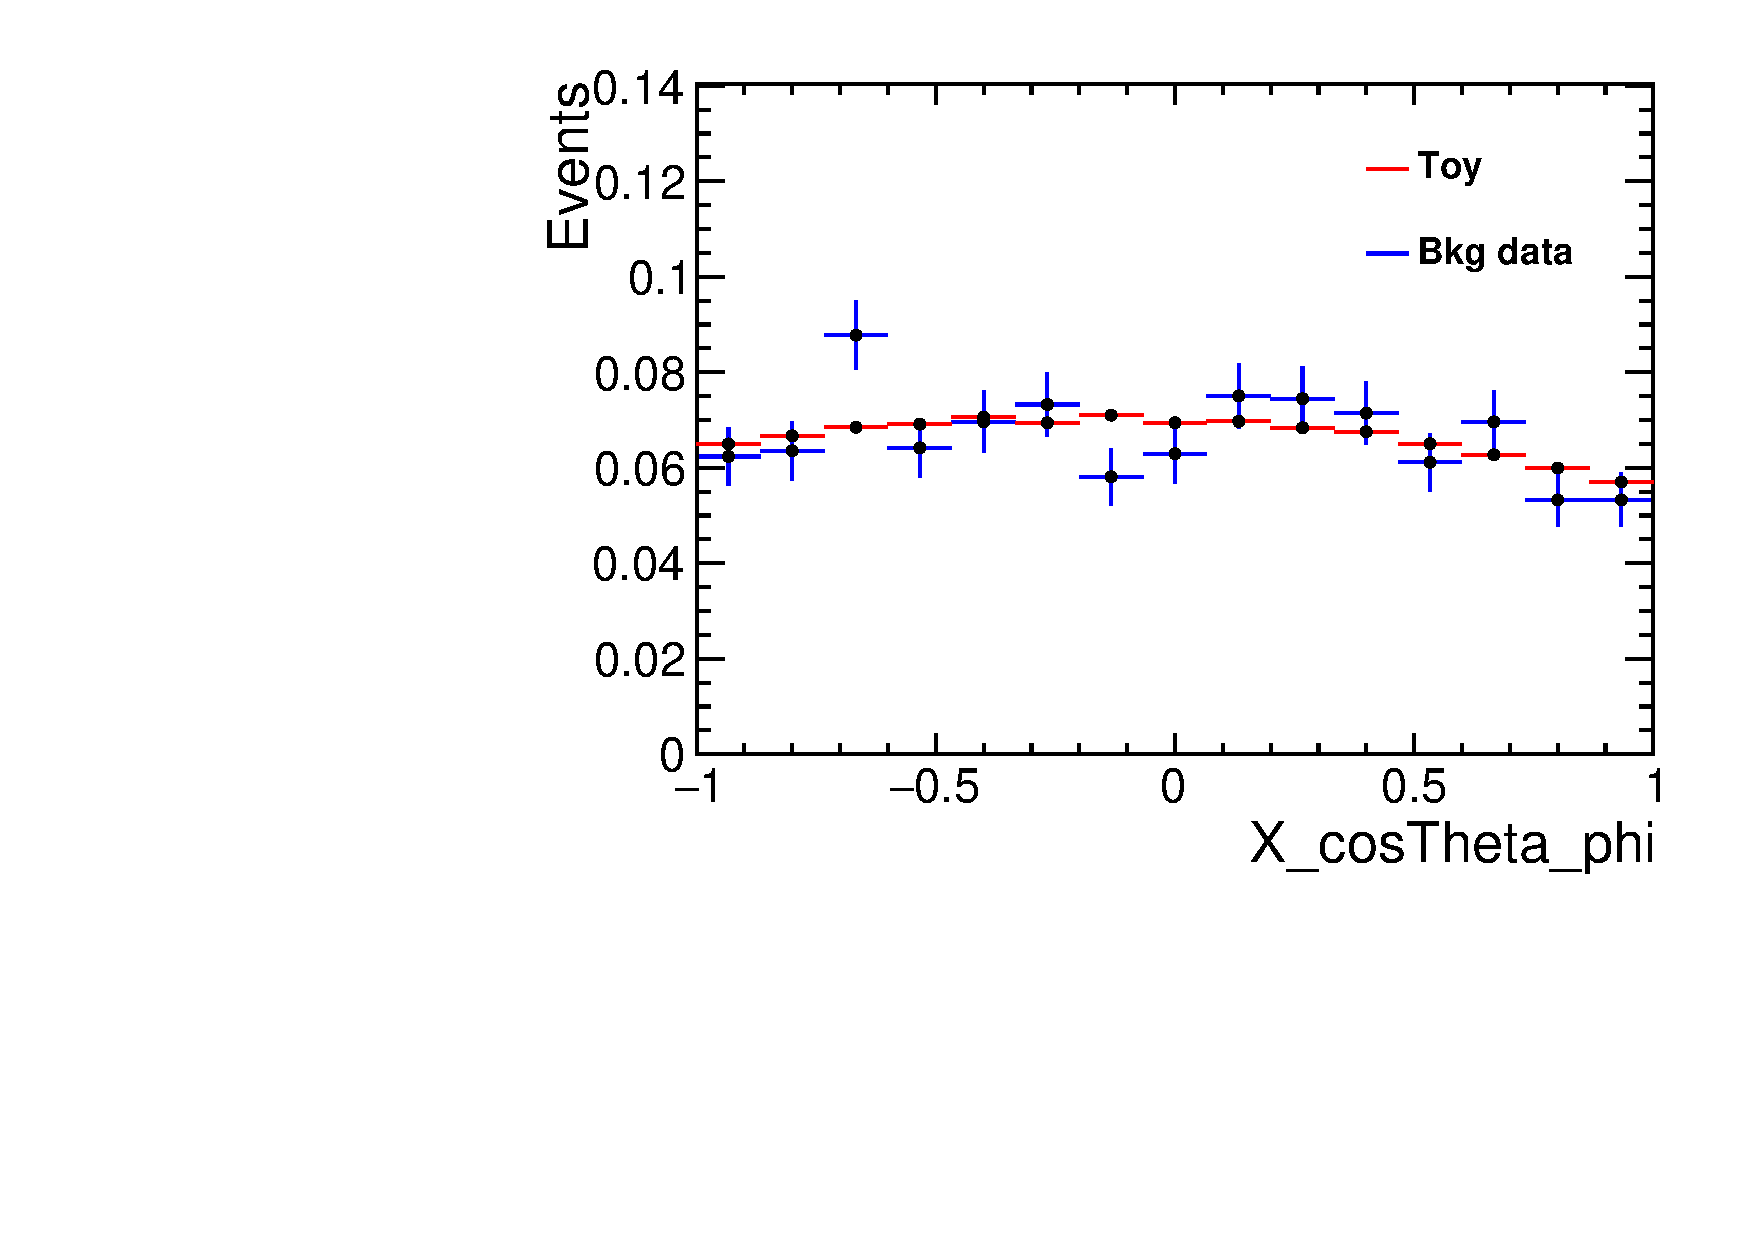
\includegraphics[width=0.3\textwidth]{Figures/03_Zcs/app_sideband/X_cosTheta_phi.pdf}%
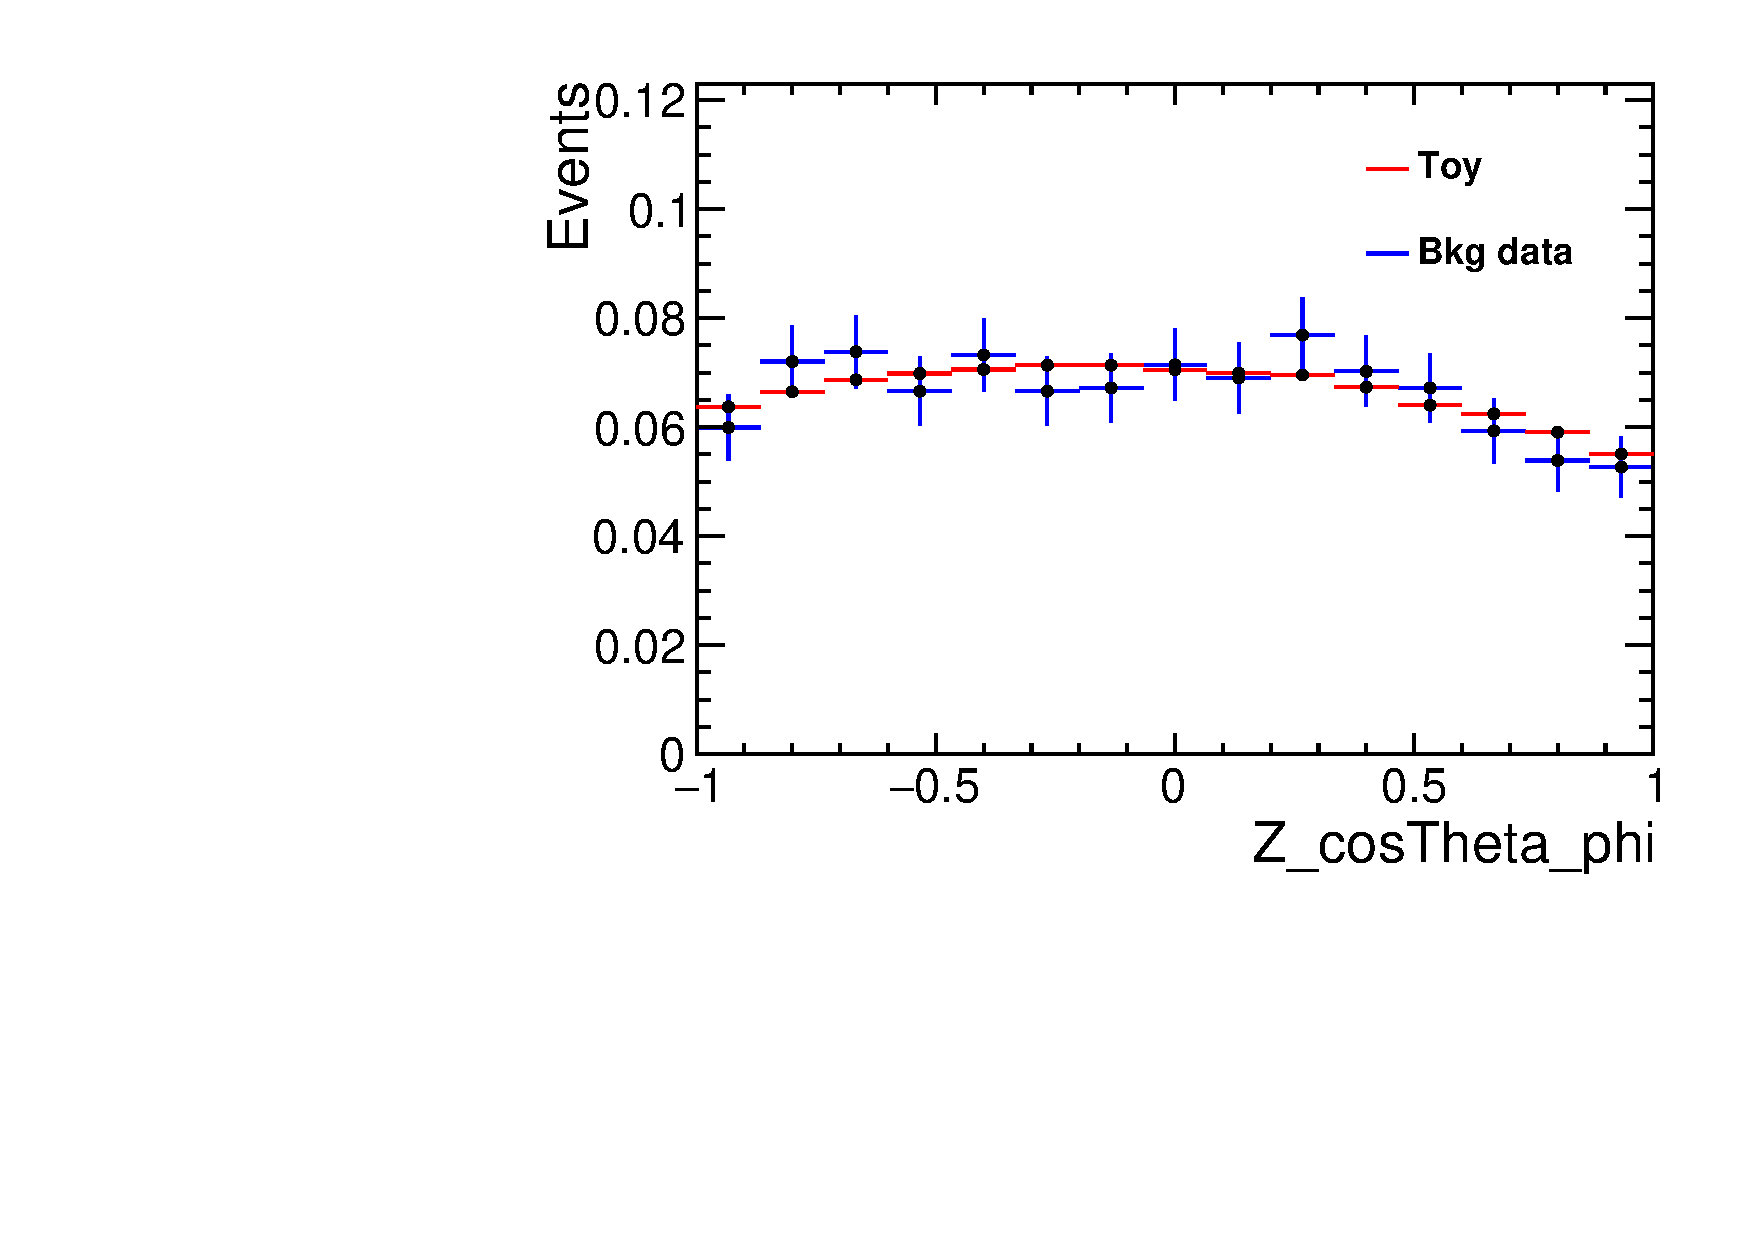
\includegraphics[width=0.3\textwidth]{Figures/03_Zcs/app_sideband/Z_cosTheta_phi.pdf}\\
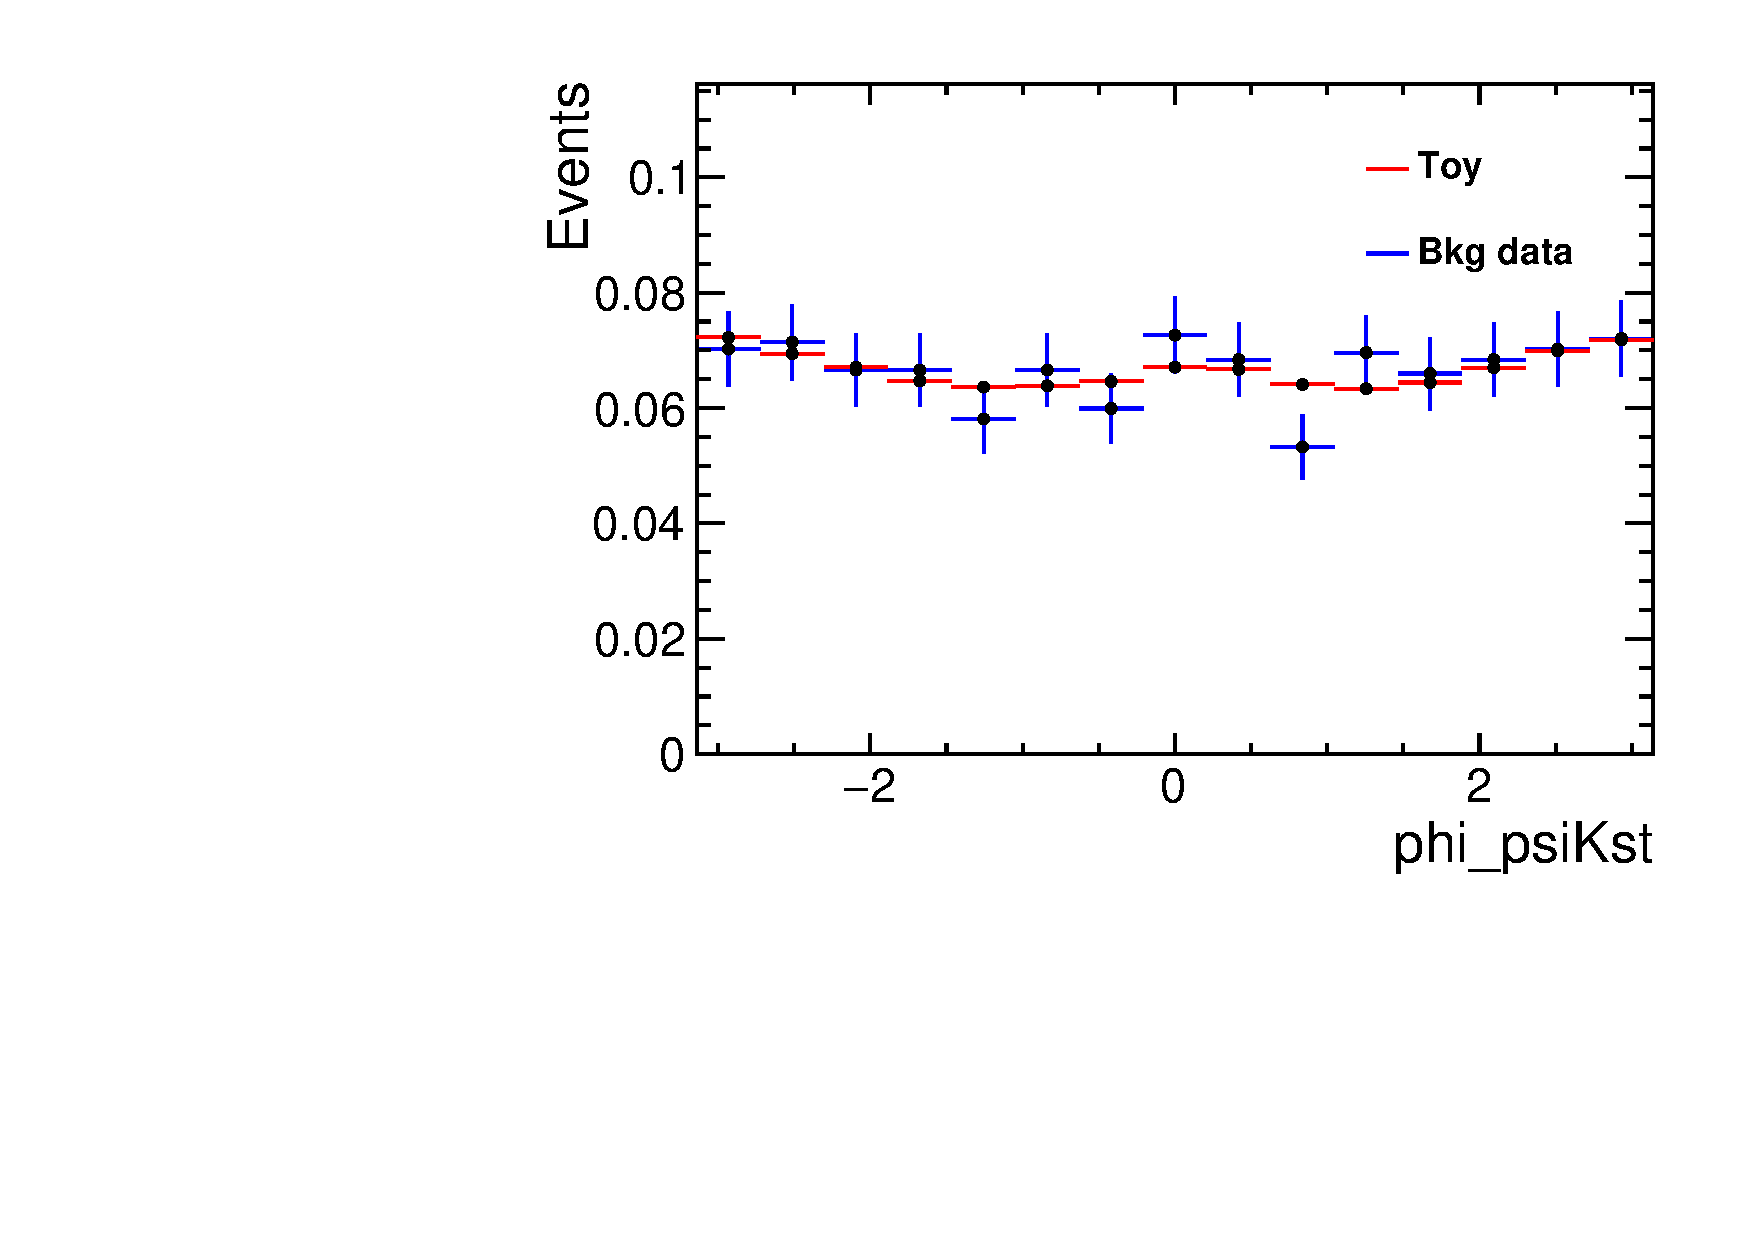
\includegraphics[width=0.3\textwidth]{Figures/03_Zcs/app_sideband/phi_psiKst.pdf}%
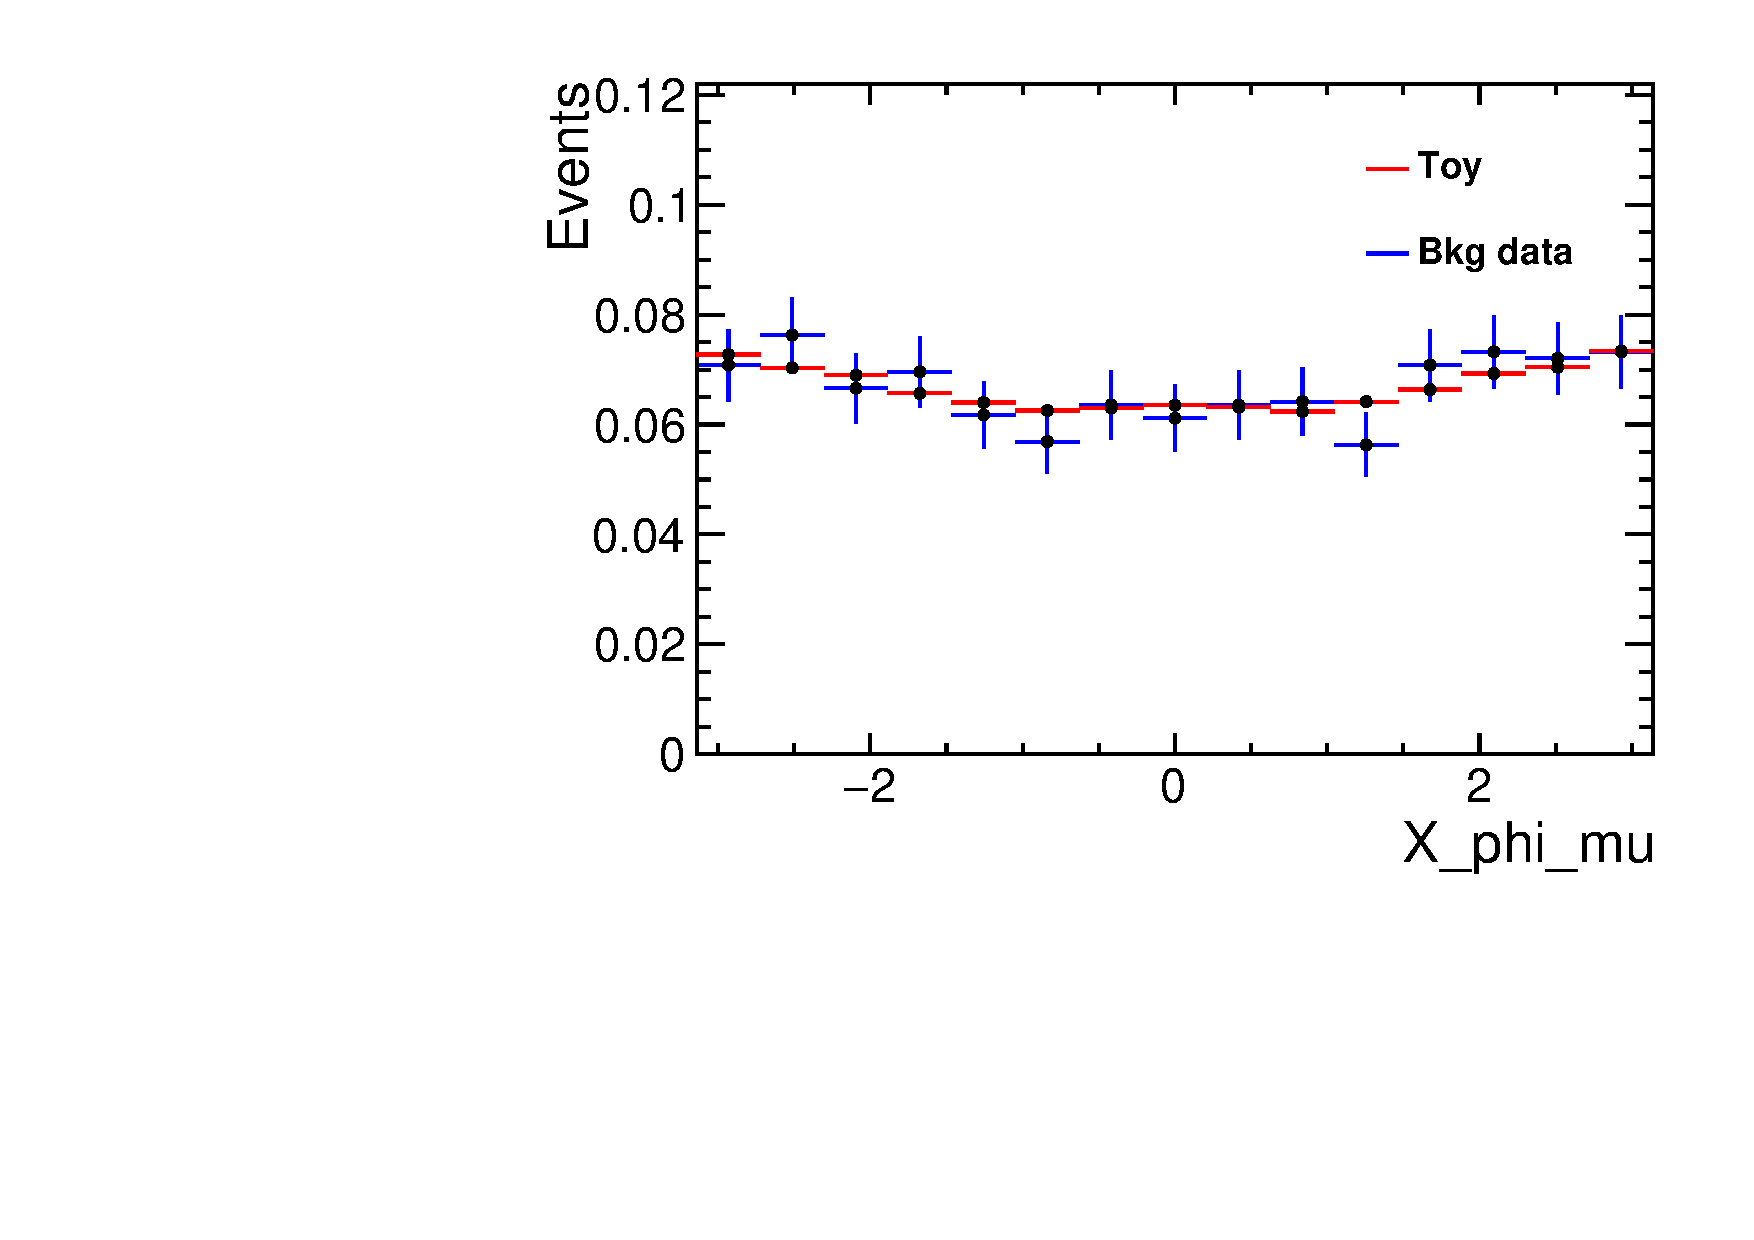
\includegraphics[width=0.3\textwidth]{Figures/03_Zcs/app_sideband/X_phi_mu.pdf}%
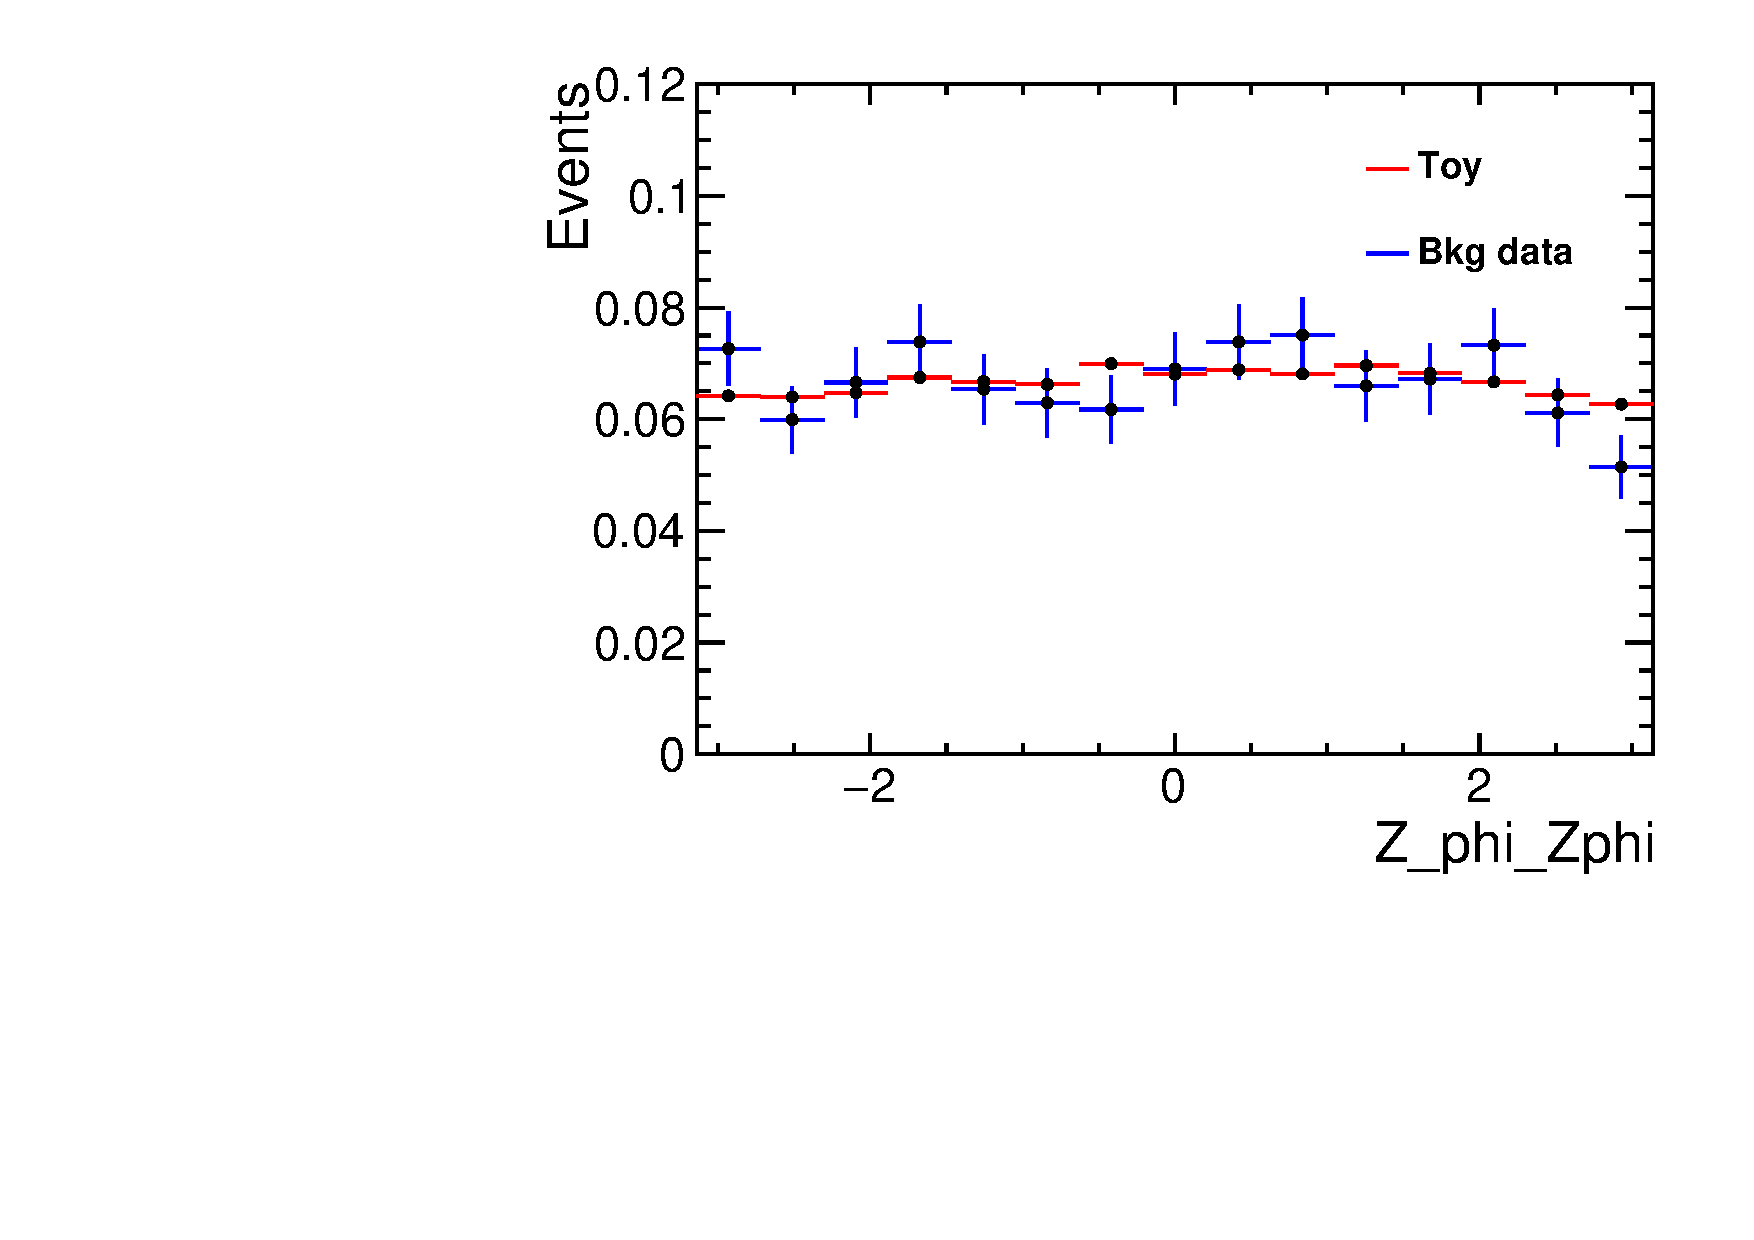
\includegraphics[width=0.3\textwidth]{Figures/03_Zcs/app_sideband/Z_phi_Zphi.pdf}\\
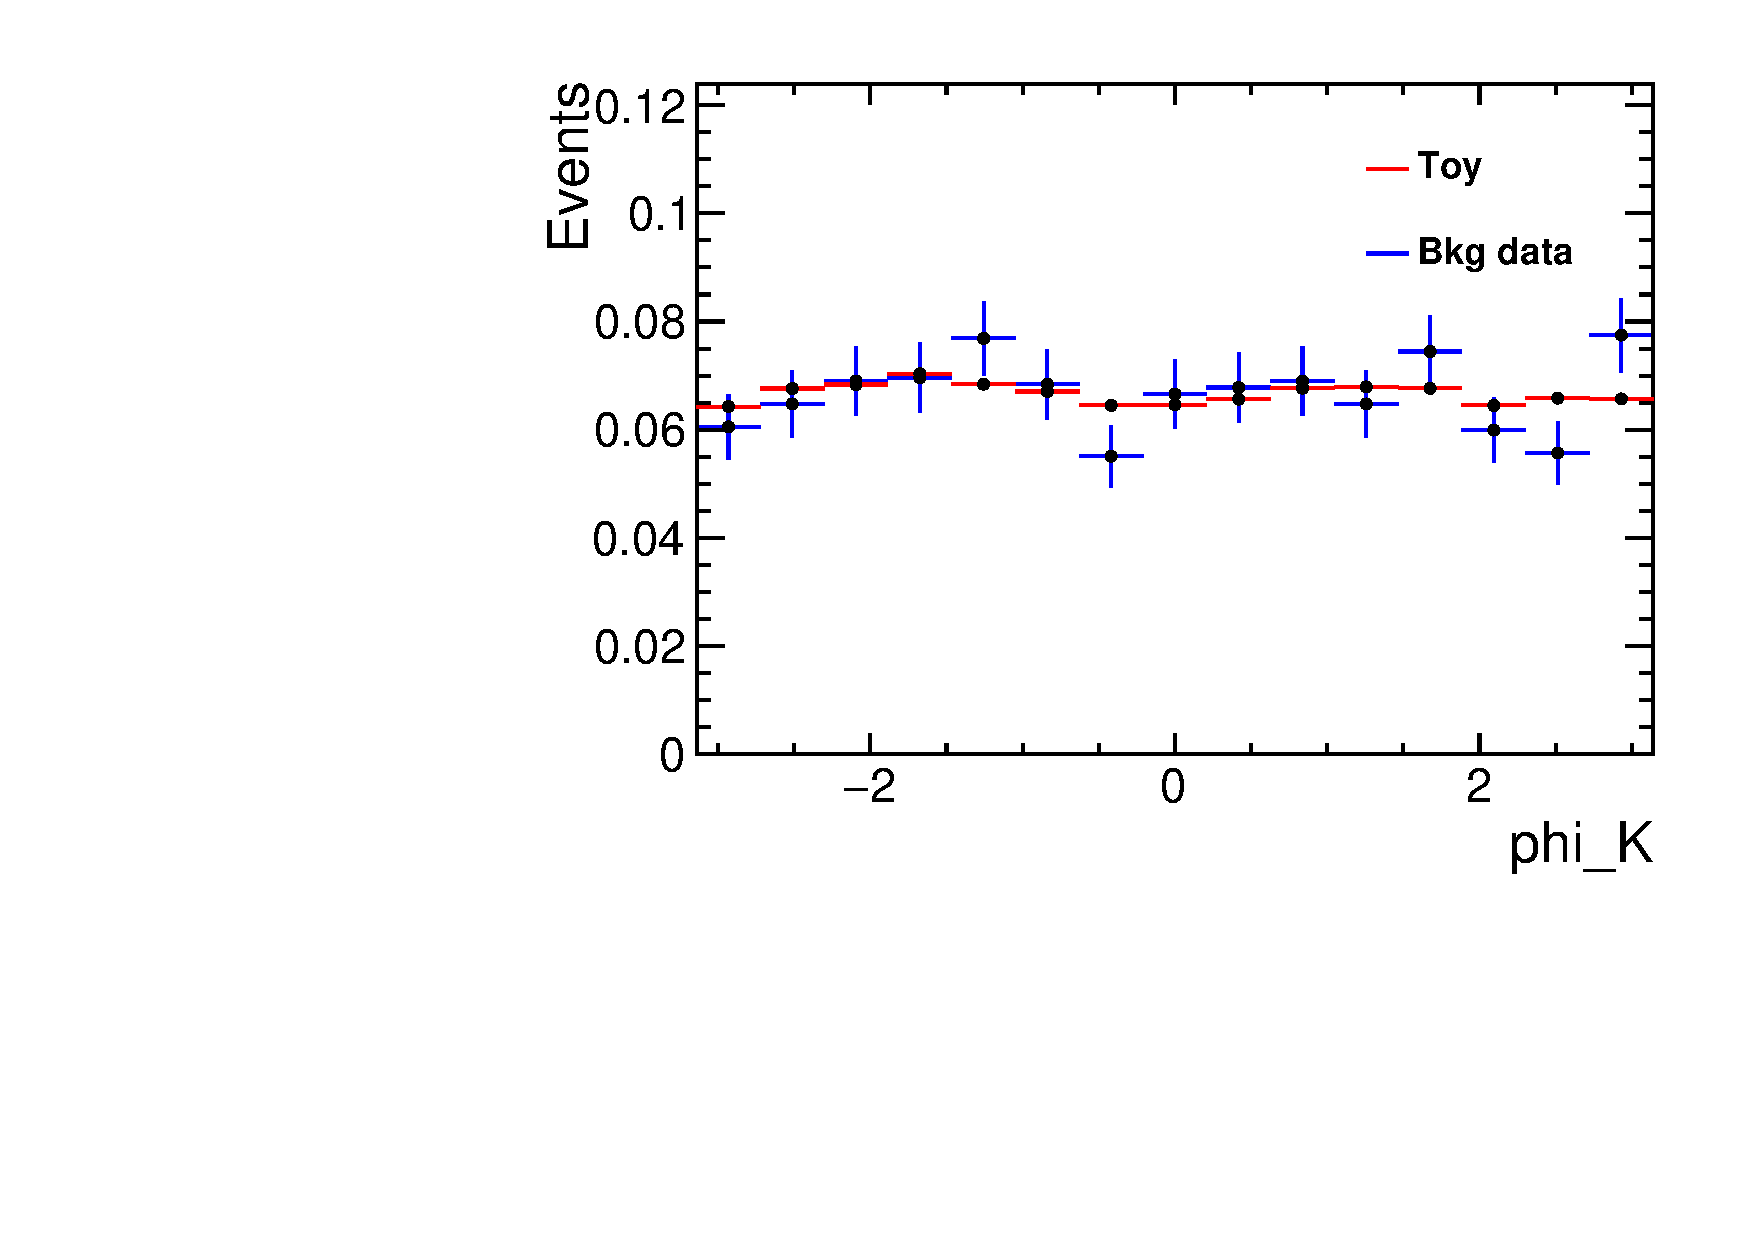
\includegraphics[width=0.3\textwidth]{Figures/03_Zcs/app_sideband/phi_K.pdf} %
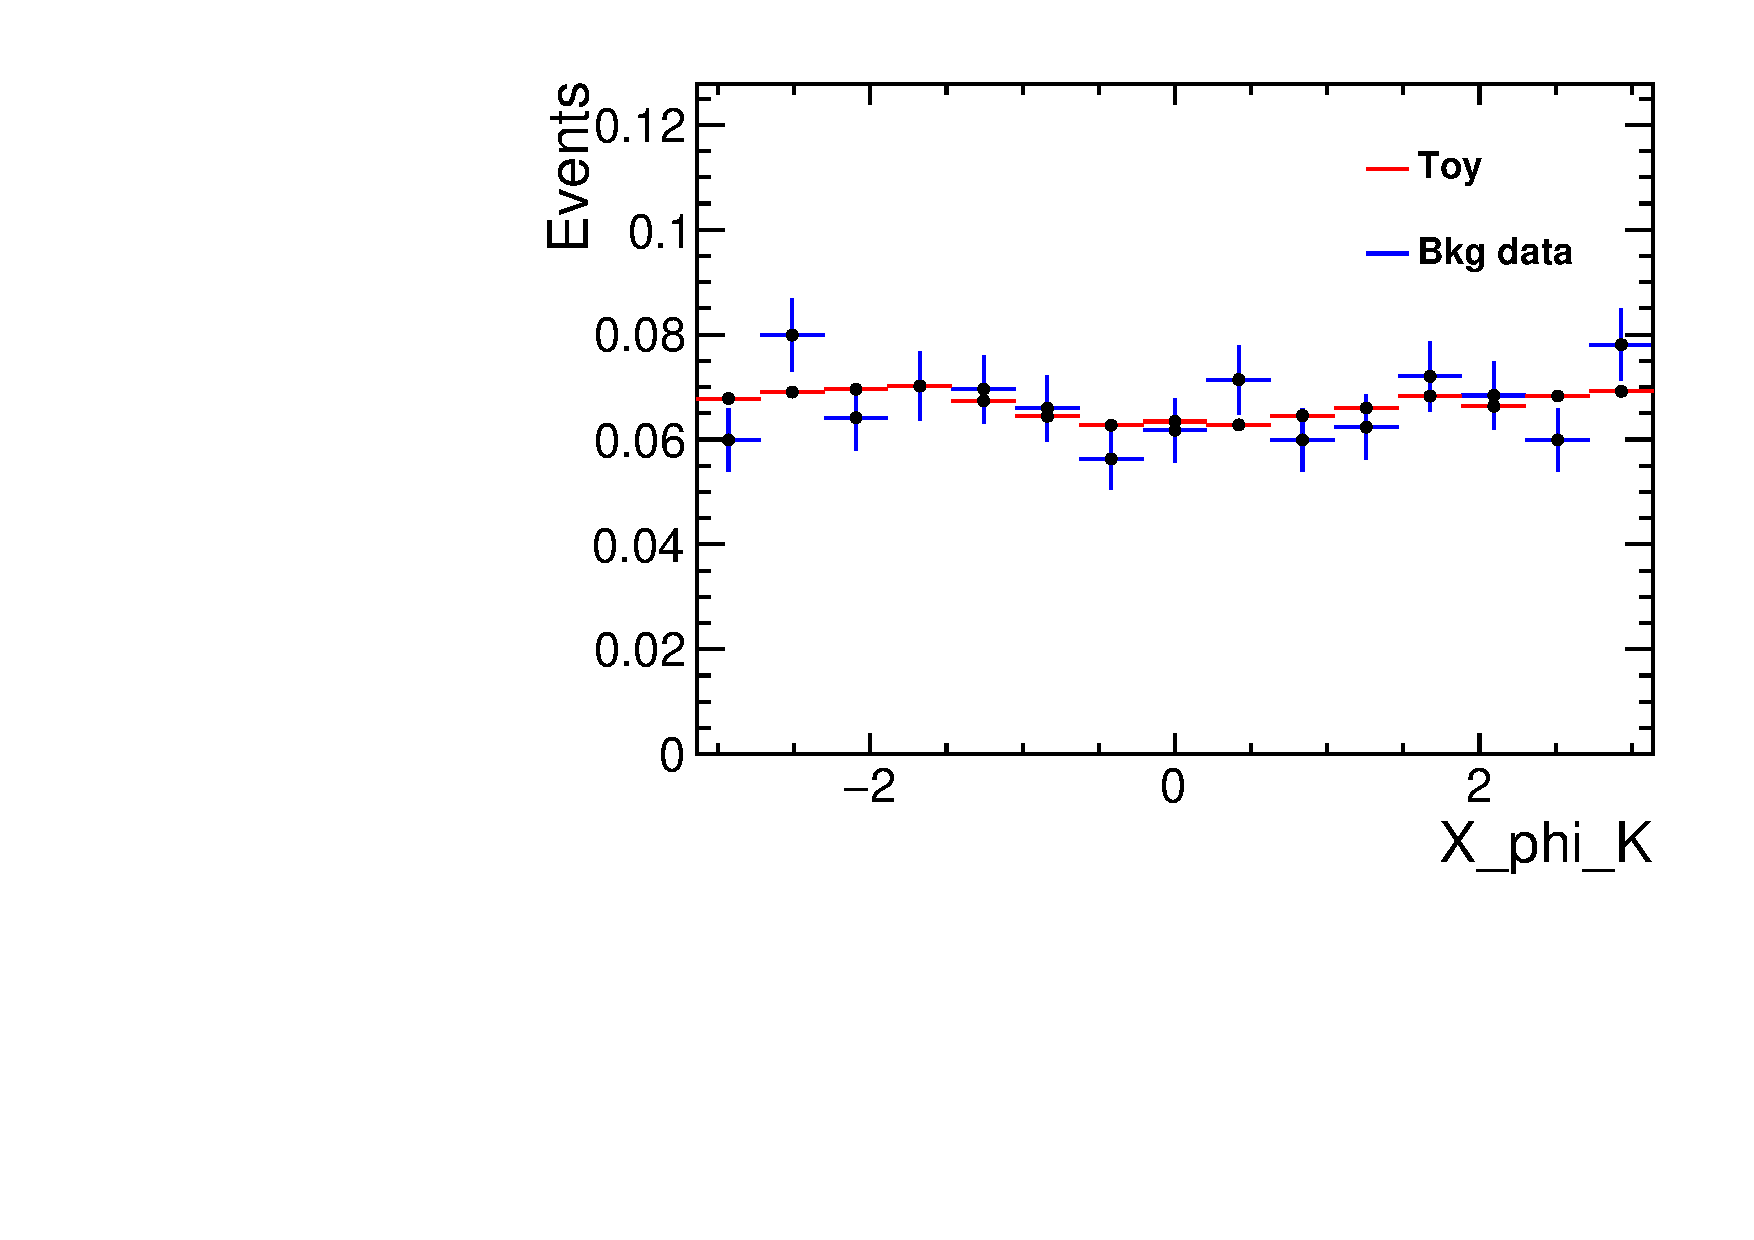
\includegraphics[width=0.3\textwidth]{Figures/03_Zcs/app_sideband/X_phi_K.pdf}%
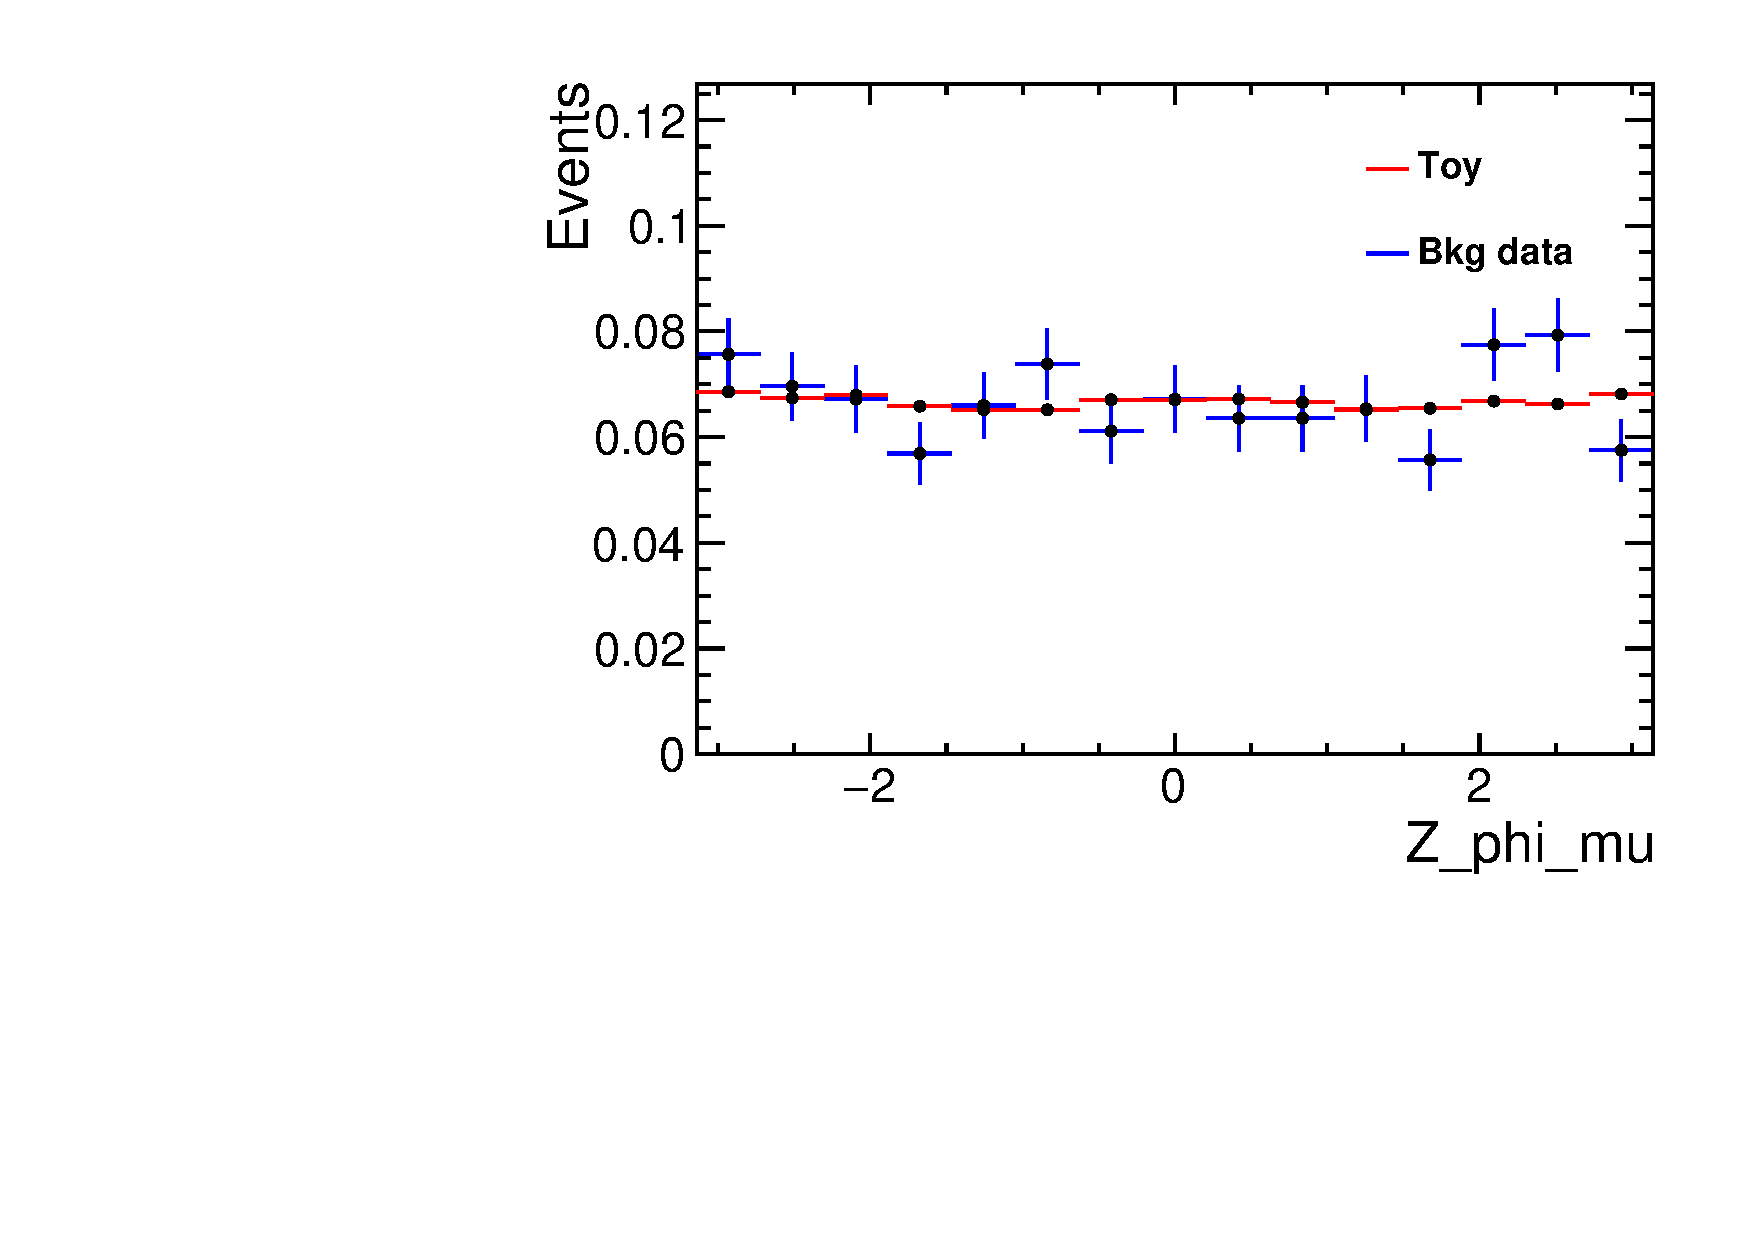
\includegraphics[width=0.3\textwidth]{Figures/03_Zcs/app_sideband/Z_phi_mu.pdf}\\
\caption{Comparison between the alternative parametrized background PDF (red dots) with the $B$ sideband data (blue dots) for all masses and angles used in nominal fit, for $K^*$ chain (left) $X$ chain (middle) and $Z_{cs}$ chain (right).}
\label{fig:mass_distribution_phi_sideband_3}
\end{figure}






% vim:ts=4:sw=4
